	\documentclass
[
a4paper,
english,
openright,                    % Kap.beginn immer rechts! (fkt. nur bei report, nicht bei article)
12pt                          % ersatzweise 12pt, wenn mehr Seiten entstehen sollen
]
{report}

%%%%%%%%%%%%%%%%%%%%%%%%%%%%%%%%%%%%%%%%%%%%%%%%%%%%%%%%%%%%%%%%%%%%%%%%%%%%%%%%%%%%%%%%%%%%%%%%%%%%%%%%%%%%
%Dokumenteneigenschaften

\newcommand{\Author}{Christian Winkler, BSc} 
\newcommand{\Title}{Expert Tuned Profile Hidden Markov Models for Primary and Secondary Structure Based Homology Prediction in Bioinformatics}
\newcommand{\Keywords}{Homology Detection, Sequence Similarity, Hidden Markov Model, Protein Alignment, Bioinformatics }
\newcommand{\Advisor}{FH-Prof Univ.- Doz. Mag. Dr. Stefan Wegenkittl}
\newcommand{\Birthdate}{16.06.1988}
\newcommand{\EnrolNum}{1510581041}
\newcommand{\VenueMonthYear}{Salzburg, September 2018}
\newcommand{\VenueDate}{Salzburg, September 2018}


%%%%%%%%%%%%%%%%%%%%%%%%%%%%%%%%%%%%%%%%%%%%%%%%%%%%%%%%%%%%%%%%%%%%%%%%%%%%%%%%%%%%%%%%%%%%%%%%%%%%%%%%%%%%
% Layout zusammengestellt von Richard Wanger im WS 2015/2016. Verschiedene Vorlagen wurden bei der Erstellung
% kombiniert und nach dem Masterleitfaden (Stand: Oktober 2015) adaptiert. Verwendung ohne Gewähr!

\usepackage{style}		%alle packages und Formatvorlagen befinden sich in dieser Datei
\usepackage{colortbl}

\usepackage{slashbox,multirow}
\usepackage{arydshln}

%%%%%%%%%%%%%%% TODO-zeug ########################
\usepackage{xargs}                      % Use more than one optional parameter in a new commands

%\newcommandx{\unsure}[2][1=]{\todo[linecolor=red,backgroundcolor=red!25,bordercolor=red,#1]{#2}}
%\newcommandx{\change}[2][1=]{\todo[linecolor=blue,backgroundcolor=blue!25,bordercolor=red,#1]{#2}}
%\newcommandx{\info}[2][1=]{\todo[linecolor=green,backgroundcolor=green!25,bordercolor=green,#1]{#2}}
%\newcommandx{\improvement}[2][1=]{\todo[linecolor=yellow,backgroundcolor=yellow!25,bordercolor=yellow,#1]{#2}}
%\newcommandx{\thiswillnotshow}[2][1=]{\todo[disable,#1]{#2}}
%\newcommand{\todobox}[1]{\fcolorbox{red}{yellow}{#1}\todo{#1}}


\newcommand{\missing}[1]{\todo[inline]{#1}}
\newcommand{\unsure}[1]{\todo[disable]{#1}}
\newcommand{\change}[1]{\todo[disable]{#1}}
\newcommand{\info}[1]{\todo[disable]{#1}}
\newcommand{\improvement}[1]{\todo[disable]{#1}}
\newcommand{\thiswillnotshow}[1]{\todo[disable]{#1}}
\newcommand{\todobox}[1]{\fcolorbox{red}{yellow}{#1}}

%%%%%%%%%%%%%%%%%%%%%



%%%%%%%%%%%%%%%%%% spezielle sachen
\newcommand{\angstrom}{\textup{\AA}}

% wegen sachen wie \textmu
\usepackage{textcomp}

% 4te Ebene in Gliedwerung
\setcounter{tocdepth}{4}
\setcounter{secnumdepth}{4}


\usepackage{rotating}
%\usepackage{rotating}
%%%%%%%%%%%%%%%%%%%%%%%%%%%%%%%%%%%%%%%%%%%%%%%%%%%%%%%%%%%%%%%%%%%%%%%%%%%%%%%%%%%%%%%%%%%%%%%%%%%%%%%%%%%%
% ORGANISATORISCHES

\begin{document}
\begin{titlepage}

\hspace{7cm}

\begin{center}
	{\Large\uppercase\expandafter{\bf MASTER'S THESIS}}\\[0.5ex]
	\vspace{1cm}
	\Large{\bf\large \Title}\\
	\vspace{1.5cm}
	\normalsize submitted to the\\
	Department of Information Technology and Systems Management\\
	at the\\
	Salzburg University of Applied Sciences\\
\end{center}

\vspace{2cm}

\begin{center}
	\normalsize by
	\\
	{
		\Large{\bf\large \Author}\\
	}
	\vspace{1cm}
	
\includegraphics[width=5cm]{BilderAllgemein/FH_Salzburg_Logo_ENG_GT.jpg}\medskip
\end{center}
	
\vspace{1cm}

\begin{tabbing}
	\hspace*{2cm}\=\hspace*{4cm}\= \kill
	\> Head of Department: \> FH-Prof.~DI Dr. Gerhard Jöchtl \\*[0.2cm]
	\> Supervisor: \> \Advisor
\end{tabbing}

\vfill	

\begin{center}
\VenueMonthYear\\
\end{center}
\end{titlepage}
\pagenumbering{roman} 
\chapter*{Declaration on Authorship}
\thispagestyle{plain}
\pagestyle{plain}

I confirm that this Master’s thesis is my own work and that I have not used any sources other than those listed in the bibliography and identified as references.

This thesis was not previously presented to another examination board and has not been published.




\vspace{3cm}

\VenueDate

\vspace{0.5cm}

\begin{tabular}{p{0.3\textwidth}p{0.32\textwidth}p{0.3\textwidth}}

\parbox[c]{1em}{
\includegraphics[width=5cm]{BilderAllgemein/SIG.JPG}} &  &  \multicolumn{1}{c}{\EnrolNum} \\ \cline{1-1} \cline{3-3}

 \Author & & Matrikelnumber

\end{tabular}
\chapter*{Common Information}
\thispagestyle{plain}
\pagestyle{plain}

\begin{tabular}{p{0.3\textwidth}p{0.65\textwidth}}

Name: & \Author \\*[0.2cm]
Institution: & Salzburg University of Applied Sciences \\*[0.2cm]
Degree Programme: & Information Technology \& Systems Management \\*[0.2cm]
Title of Thesis: & \Title \\*[0.2cm]
Keywords: & \Keywords  \\*[0.2cm]
Supervisor: & \Advisor

\end{tabular}

\section*{\Large\bfseries Abstract}



Protein homology classification is an important task to better understand proteins whose three-dimensional structure and function are not obvious. Current methods that rely on the primary structure of a protein do not always find distant homologous relationships between proteins.  
%
This thesis examines the usage of secondary structure information in profile Hidden Markov Models to improve the classification accuracy in protein family prediction.
%
This is done by extending the emission frequencies of the primary structure by secondary structure frequencies. A generalized mixed frequency set is generated using optimized weighting techniques. 
The secondary structure is determined by the three-dimensional structure, if available, or predicted from the primary structure.
%
To assess the effectiveness of the different weighting methods, the implementation has been tested with 69 selected sequence alignments, representing distant related families. These sequences have been scored against the SCOP database to determine the accuracy of finding distant homologous relationships between proteins. 
%
Results show that the integration of secondary structure information improves the accuracy of homology prediction.  
%\include{04Danksagung}

%%%%%%%%%%%%%%%%%%%%%%%%%%%%%%%%%%%%%%%%%%%%%%%%%%%%%%%%%%%%%%%%%%%%%%%%%%%%%%%%%%%%%%%%%%%%%%%%%%%%%%%%%%%%
%VERZEICHNISSE

\tableofcontents
\protect \addcontentsline{toc}{chapter}{Contents}

\renewcommand{\nomname}{List of Abbreviations}
\chapter*{List of Abbreviations}
\addcontentsline{toc}{chapter}{List of Abbreviations} 
\pagestyle{plain}

% insert longest word in [] for alignment
\begin{acronym}[UniProtKB]
 \acro{AA}{Amino Acid}
 \acro{angstrom}[\AA] {\AA ngstrom}	
 \acro{ASA} {Accessible Surface Area}
 \acro{AUC} {Area Under the Curve}

 \acro{CCD} {charge-coupled device}		% entfernen?
 \acro{DNA} {deoxyribonucleic acid}
 \acro{DSSP}{Dictionary of Secondary Structures in Proteins}

 \acro{FPR} {false positive rate}
 
 \acro{GUI}{graphical user interface}
 
 \acro{HMM}{Hidden Markov Model}
 
 \acro{MSA}{multiple sequence alignment}
 
 \acro{MStA}{multiple structure alignment}
 \acro{NMR}{Nuclear Magnetic Resonance}
 \acro{NN}{neural network}

 \acro{PCA} {principal component analysis}
 \acrodefplural{PCA}[PCA]{Principal component analysis}
 
 \acro{PDB}{Protein Data Bank} 
 \acro{PHD}{Profile Network from HeiDelberg}
 \acro{pHMM}{profile Hidden Markov Model} 
 \acro{PP}{physio-chemical property}
 \acrodefplural{PP}{physio-chemical properties}
 
 
 \acro{PSSM}{Position-Specific Scoring Matrix}
 \acro{RNA}{ribonucleic acid}
 \acro{ROC} {Receiver Operating Characteristic}
 \acro{RSA} {Residue Solvent Area}
 \acro{SCOP}{Structural Classification of Proteins}
 \acro{SCOPe}{Structural Classification of \mbox{Proteins--extended}} 
 
 \acro{SID} {SCOP Identifier}
 %\acro{SS}{Secondary Structure}
 \acro{SVM}	{support vector machine}
	
 \acro{TPR} {true positive rate}

 \acro{UniProtKB} {UniProt Knowledgebase}  
 \acro{XRC} {x-ray crystallography}

%\acro {EMR} {electromagnetic radiation}
 
\end{acronym}


\listoffigures
\protect \addcontentsline{toc}{chapter}{List of Figures}

\listoftables
\protect \addcontentsline{toc}{chapter}{List of Tables}
\newpage
%\lstlistoflistings
%\protect \addcontentsline{toc}{chapter}{Listings}

%%%%%%%%%%%%%%%%%%%%%%%%%%%%%%%%%%%%%%%%%%%%%%%%%%%%%%%%%%%%%%%%%%%%%%%%%%%%%%%%%%%%%%%%%%%%%%%%%%%%%%%%%%%%
%INHALT

\setcounter{page}{0}
    \pagenumbering{arabic}
    \setcounter{page}{1}
\setcounter{page}{0}
\pagenumbering{arabic}
\setcounter{page}{1}

\chapter{Introduction}
\label{ch:Introduction}


\thispagestyle{standard}
\pagestyle{standard}


Proteins are the essential building blocks of all forms of life. They can be found in all living organisms and play a key role in different functions of life. All proteins are made up of one or more chains arranged together in specific amino acid sequences. Although these sequences are built from a set of just 20 different elements, they can arrange in an innumerable number of configurations. With regard to the human body, there are more than 20,000 different proteins. 

\section{Research purpose}

Understanding the function of  proteins is a crucial task in bioinformatics. Each new discovery of a protein structure and its function provides more knowledge about how the macro-molecular mechanisms of life work. This knowledge is important in many different areas, such as the  pharmaceutical industry, where it is necessary to know the shape of viruses or bacteria in order to design drugs to counter them. Another application is biotechnology, which aims to develop new technologies, such as \mbox{self-assembling} organic solar cells. 

Although at present  determining protein sequences is a simple and straightforward task, it produces an enormous amount of protein sequence data. Gaining information about the three-dimensional shape of the protein is a slow and strenuous task. Several prediction methods based on the sequence data already provide a good indication of the structure of certain parts of a protein. Nevertheless, prediction of the complete structure remains an unsolved problem. 
One approach to gain further information about the function of a protein is to find evolutionary connections, also known as homology, to other known structures. Proteins with the same functions are likely related to each other, as they might have originated from a common ancestor. These connections can be inferred according to similarities in the sequence and structure and thus according to similar functions. However, the conservation of two homologous sequences is not always clear, as due to mutations several amino acids or even longer sections in the chain may have changed over generations. 




This thesis investigates the use of \ac{pHMM} in protein family classification. Specifically, the common approach, which uses only the primary structure to build a \ac{pHMM} and score sequences against it, will be extended to make use of secondary structure information.  
There are particular cases in which protein homology is not well presented by sequence similarity in certain parts of the protein. It is expected that stability, with respect to the secondary structure, increases the classification quality.


\section{Overview}
Chapter \ref{ch:selectedBG} provides an overview of the areas of bioinformatics relevant to this thesis. These include topics such as protein composition, protein structure and function, and the fundamentals of \ac{pHMM}.

Chapter \ref{ch:PSD} discusses protein structure determination on its different levels. A special focus is on methods for secondary structure determination.

In Chapter \ref{ch:implement}, the implementation of various methods for \ac{pHMM} using secondary structure information in the software package \textit{HMModeler} is described.  Based on the theoretical background, this chapter covers the steps from an \ac{MSA}, determining secondary structure, building a \ac{pHMM} and scoring sequences against it.

Chapter \ref{ch:evaluate} evaluates the implementation based on various datasets. In particular, different methods for including secondary structure information with various parameters are compared to one another.

Finally, Chapter  \ref{ch:conclusion} concludes by providing a short summary of the thesis' findings.



\chapter{Selected Background Information}
\label{ch:selectedBG}

Bioinformatics covers a wide range of scientific fields, such as biology, chemistry and computer science. This chapter gives a short introduction to the areas of bioinformatics relevant to the methods and implementation used in later chapters. 


\section{Proteins}

Proteins play a key role in almost all biological activity. Proteins are large biological polymers composed of one or more chains of amino acids. These amino acids are held together by spatial bonds called peptide bonds. Further information about the material described in this section can be found in \cite{ Nelson.2013, Gromiha.2010, Berg.imp.2002}.

\subsection{Amino Acids}
\label{ssec:AminoAcid}

Amino acids are the basic building blocks of proteins. Each amino acid consists of a central $\alpha$ carbon ($C_\alpha$) bound to:

\begin{itemize}
\item  a carboxyl group ($COOH$)

\item an amino group ($NH_2$)

\item a hydrogen atom ($H$)

\item a distinct side chain (or $R$-group)
\end{itemize}

Variation in the side chain defines the 20 common amino acids found in protein molecules. For instance, if the side chain contains just one hydrogen atom, the amino acid is glycine, while the side chain $CO_2OH$ forms the amino acid serine. Table \ref{tab:AAlist} lists the 20 common amino acids found in proteins with their assigned three-letter abbreviations and one-letter symbols, as defined in \cite{IUPACIUBJointCommissiononBiochemicalNomenclature.1984}. The abbreviations and one-letter symbols are used to simplify computing with amino acid chains.


\begin{table}[h!]
	\centering
	\begin{tabular}{|l|c|c|}
		\firsthline
		Amino acid	  & Abbreviation &
		 One-letter symbol \\ \hline
		Alanine       & Ala  & A   \\
		Arginine      & Arg & R \\
		Asparagine    & Asn & N \\
		Aspartic acid \qquad & Asp & D \\
		Cysteine      & Cys & C \\
		Glutamic acid & Glu & E \\
		Glutamine     & Gln & Q \\
		Glycine       & Gly & G \\
		Histidine     & His & H \\
		Isoleucine    & Ile & I \\
		Leucine       & Leu & L \\
		Lysine        & Lys & K \\
		Methionine    & Met & M \\
		Phenylalanine \quad & Phe & F \\
		Proline       & Pro & P \\
		Serine        & Ser & S \\
		Threonine     & Thr & T \\
		Tryptophan    & Trp & W \\
		Tyrosine      & Tyr & Y \\
		Valine        & Val & V  \\\hline
	\end{tabular}
	\caption[The 20 common amino acids.]{The 20 common amino acids of proteins with their three-letter abbreviations and one-letter symbols \cite{IUPACIUBJointCommissiononBiochemicalNomenclature.1984}.}
 \label{tab:AAlist}
\end{table}


Several additional symbols for so-called ``ambiguous amino acids'' are also defined. These are placeholders for positions in a protein where the exact type of a single amino acid cannot be experimentally determined. For example, the symbol B stands for either aspartic acid or asparagine, while X stands for any one of the 20 common amino acids.






\subsection{Physio-chemical Properties of Amino Acids}
\label{ssec:ppaa}

The side chains of amino acids give them specific properties that influence how each amino acid can interact with its surroundings. 
In \cite{Meiler.2001}, Meiler et al. collected seven unique \acp{PP} for each of the 20 amino acid molecules. These are as follows:



\begin{itemize}
\item \textit{Steric parameter:} The steric parameter is the graph-shape index that characterizes the molecular shape of the molecule through its possible deformations.


\item \textit{Volume:}  The volume is described as the normalized molecular volume occupied by the atoms of an amino acid.

\item \textit{Isoelectric point:} The isoelectric point is the pH-value of a solution in which the amino acid exists in a neutral form, where it is neither positively nor negatively charged. 

\item \textit{Polarizability:} The polarizability is the dynamic response of the molecule to external magnetic fields in order to form instantaneous dipoles. 

\item \textit{Hydrophobicity:}  Hydrophobicity describes the possibility of interactions between polar solvents like water and the side chain of the amino acid. A high hydrophobicity indicates that the residue has a low ability to bind with the solvent.

\item \textit{Helix probability:} This is the probability of an amino acid being identified as $\alpha$-helix in the secondary structure. 

\item \textit{Sheet probability:} This is the probability of an amino acid being identified as $\beta$-sheet in the secondary structure. 

\end{itemize}

The values for these seven \acp{PP} for the 20 amino acids can be found in Appendix \ref{app:PPAA}.



\subsection{Polypeptides}

Two amino acids can form a dipeptide through a covalent chemical bond. This bond is formed through the cleavage of a water molecule ($H_2O$) from the carboxyl group of one amino acid  and the amino group of another. The resulting $CO-NH$ bond is called a \textit{peptide bond} (see Figure \ref{fig:dipeptide}). 

\begin{figure}[b!]
	\begin{center}
		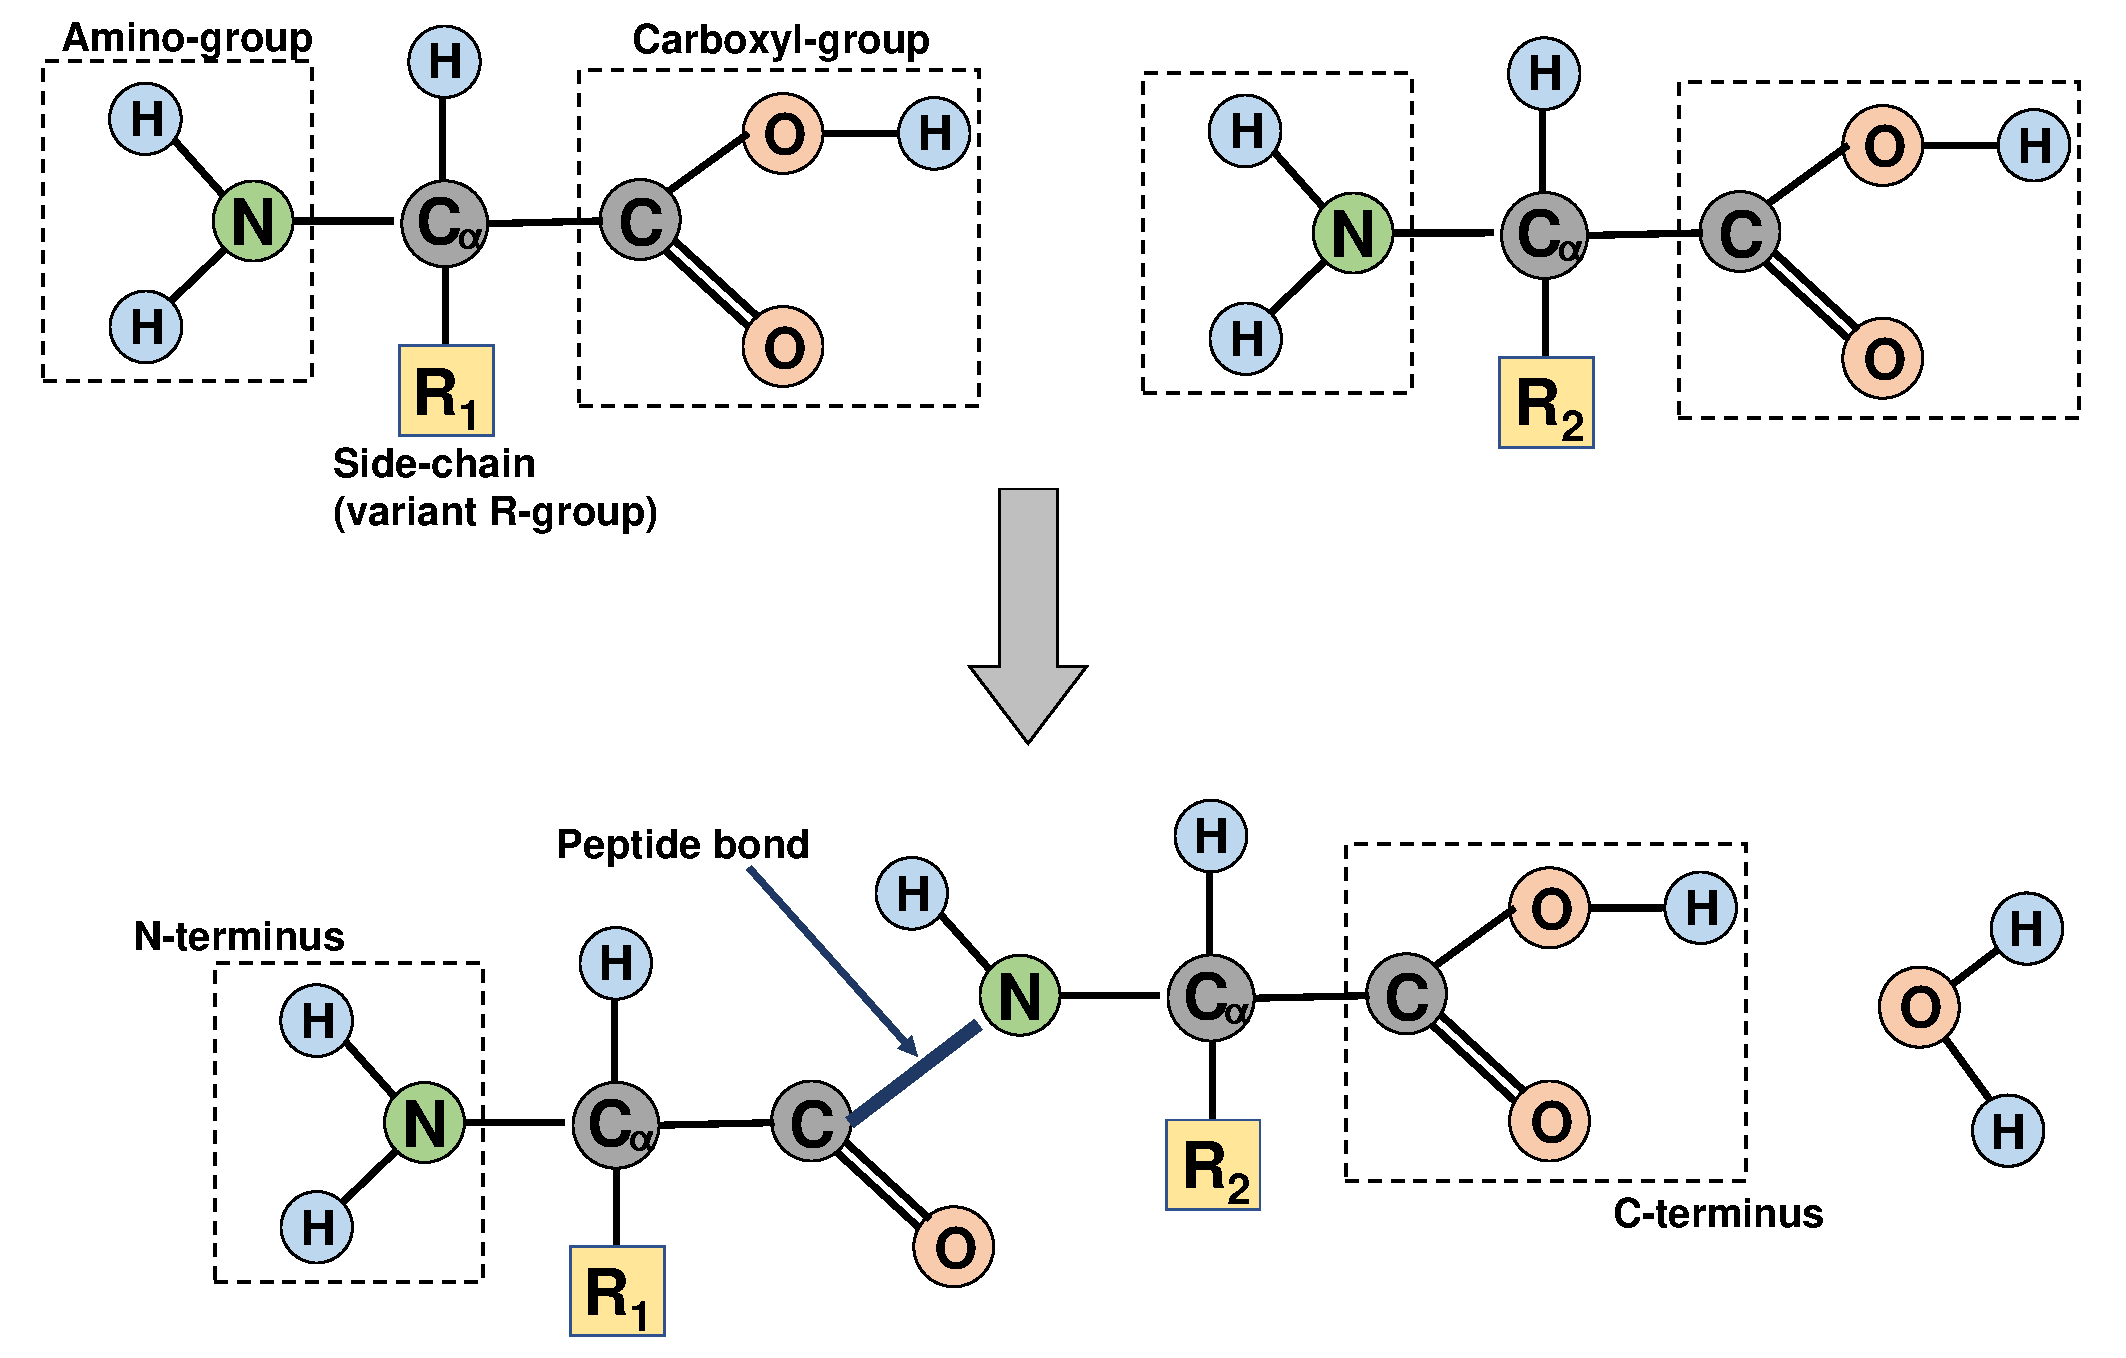
\includegraphics[width=0.94\textwidth]{fig/peptideBond}
	\end{center}
	\caption{Dipeptide forming from the condensation of two amino acids. }
	\label{fig:dipeptide}
\end{figure}

Peptide bonds can extend into peptide chains with a size of up to several thousand  amino acid residues. For example, the longest known and experimentally determined peptide chain is \textit{titin},  with almost 36,000 amino acid residues\footnote{Titin UniProt entry: \url{https://www.uniprot.org/uniparc/UPI000264F4A1} (accessed July 18, 2018).}. However, the average sequence length is 336 amino acid residues\footnote{UniProtKB Statistics: \url{https://www.ebi.ac.uk/uniprot/TrEMBLstats} (accessed July 18, 2018).}.

 By convention, the reading direction of a polypeptide chain is defined from the N- to the C-terminus. The N-terminus refers to the free amino group at one end and the \mbox{C-terminus} to the free carboxyl group at the other end of the chain. 
 Unfolded sequences with up to 50 residues are generally referred to as peptides. For longer sequences, the term ``polypeptide'' is used. 
 One or more polypeptides that together form a biologically functioning unit when folded into a three-dimensional structure are called a protein. 

 



\subsection{Protein Backbone}
\label{ssec:backbone}

The continuous repeated chain of the central covalent bounded atoms \mbox{(-NH-C$_\alpha$-CO-)} in a polypeptide forms the main chain and is referred to as the backbone. 
For each residue in a polypeptide backbone, the three dihedral  angles $\phi$, $\psi$, $\omega$ define its orientation in space. As shown in Figure \ref{fig:dihedral}, the dihedral angle is the torsional angle at the intersection of two planes over four consecutive atoms of the backbone, with the angle $\phi$ between NH and C$_\alpha$, $\psi$  between C$_\alpha$ and CO, and $\omega$ at the peptide bond, from one amino acid residue to the next. 



\begin{figure}[h!]
	\begin{center}
		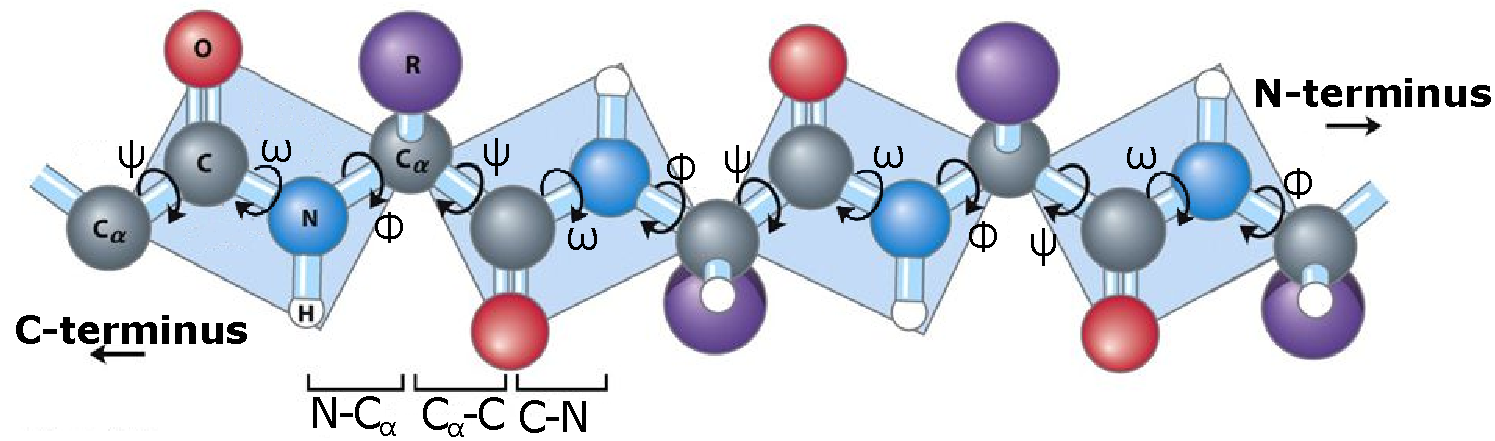
\includegraphics[width=0.8\textwidth]{fig/dihedral}
	\end{center}
	\caption[The dihedral angles $\phi$, $\psi$, $\omega$ in a polypeptide.]{The dihedral angles $\phi$, $\psi$, $\omega$ in a polypeptide, adapted from \cite{Nelson.2013}.}
	
	\label{fig:dihedral}
\end{figure} 

Although the dihedral angles are measured in values from -180$^{\circ}$ to +180$^{\circ}$, the rotation is restricted by several factors.  
Peptide bonds have a partial double-bonded character because they resonate between a single-bond and double-bond state. 
This restricts the rotation angle $\omega$ to two possible configurations, usually with an angle of 180$^{\circ}$ or in some rare cases 0$^{\circ}$. 
The other two angles $\phi$ and $\psi$ are single-bonded and can therefore in principle rotate freely. 
However, the possible orientations are limited by the variant R-group, as atoms of certain side chains may interfere with the backbone. Ramachandran plots are used to display the statistical distribution of the combination of possible conformations for both dihedral angles of each residue.


The Ramachandran plot in Figure \ref{fig:ramachandran} shows the freely available conformation space of amino acid residues, based on the atoms' \textit{van der Waals} radii\footnote{The van der Waals radius is the spherical region of an atom that represents the distance that another atom approaches before the repulsive force becomes too strong.}. 
Green regions mark orientations without interference. The light green regions are less common, especially for residues with larger side chains, but are a possible conformation with reduced van der Waals radii. Except for glycine, white regions are not malleable. Glycine, with its small side chain of just one hydrogen atom, has a broader flexibility and therefore can orient itself in all four quadrants of the Ramachandran plot.

\begin{figure}[h]
	\begin{center}
		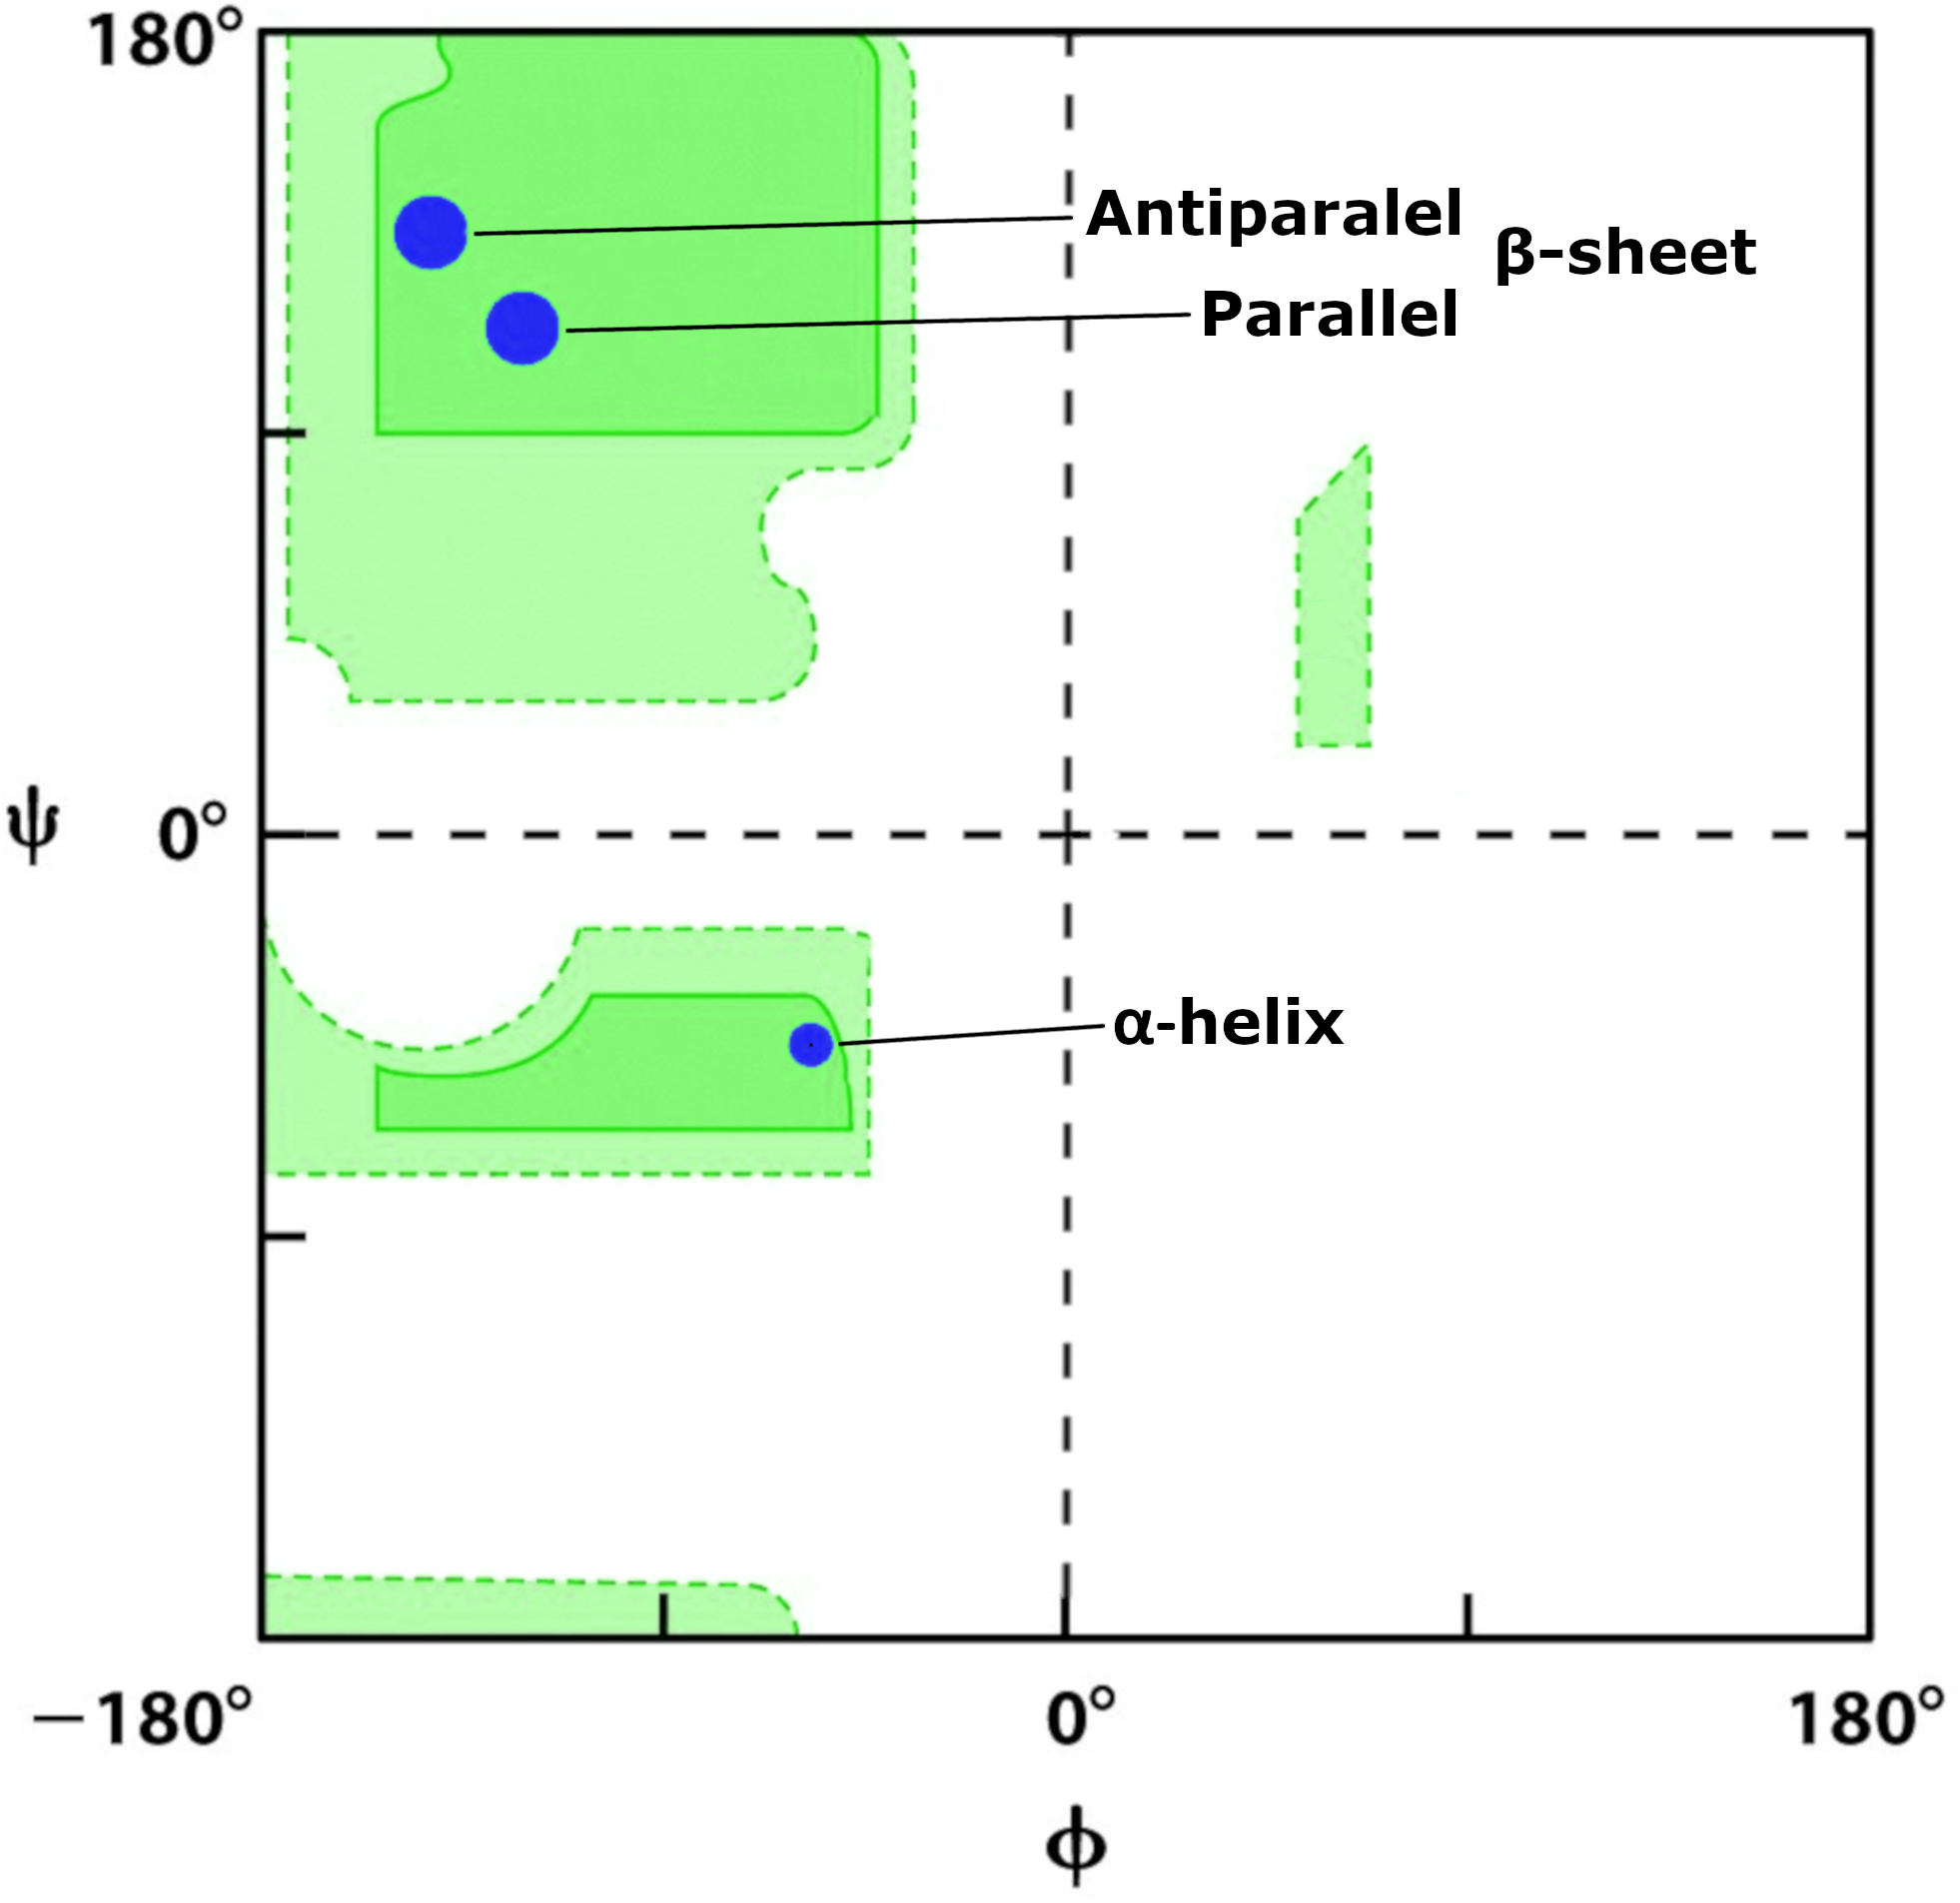
\includegraphics[width=0.54\textwidth]{fig/Ramaplot}
	\end{center}
	
	\caption[Ramachandran plot marking possible conformation of amino acid residues for the dihedral angles.]{Ramachandran plot marking possible conformation of amino acid residues for the dihedral angles $\phi$ on the horizontal and $\psi$ on the vertical axis, adapted from \cite{Nelson.2013}.}
	\label{fig:ramachandran}
\end{figure} 
 
 
% ################################################################
%%----------------------   PROTEIN STRUCTURE    ------------------
% ################################################################
\subsection{Protein Structure}


The shape of a protein is critical to its function. When stretched out, polypeptide chains have no functional activity. They become active when arranged in their stable three-dimensional structure, which is dictated by the chain's amino acid sequence. The protein structure can be divided into four hierarchical levels: primary, secondary, tertiary, and quaternary. These four levels, described in more detail below, are shown in Figure \ref{fig:protein}.

\begin{figure}[h!]
	\begin{center}
		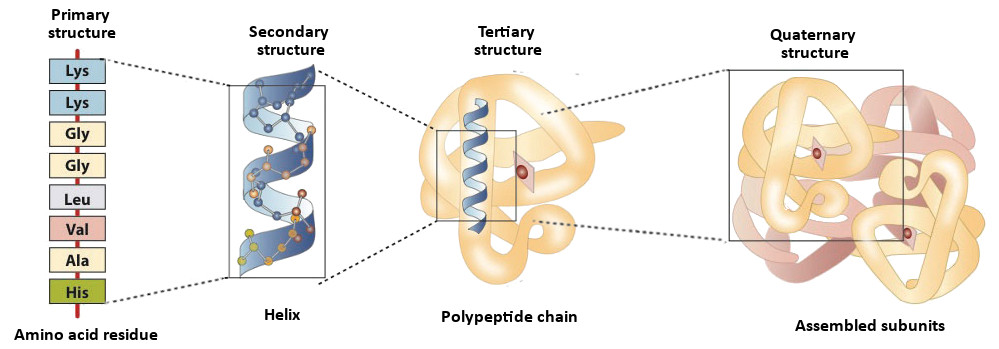
\includegraphics[width=1\textwidth]{fig/BspStruct.jpg}
	\end{center}
	\caption[The four levels of structure in proteins.]{The four levels of structure in proteins \cite{Nelson.2013}.}
	\label{fig:protein}
\end{figure}



The \textbf{primary structure} is represented by the linear sequence of amino acids within a polypeptide connected by peptide bonds, where each element corresponds  to one of the 20 amino acids described in  Section \ref{ssec:AminoAcid}. The primary structure of a polypeptide can  be determined from protein sequencing methods such as spectrometry. 

The \textbf{secondary structure} is defined by the local folding patterns of a region of the protein over a short range of amino acids in a polypeptide. The secondary structure is mainly dependent on the primary structure, which is stabilized by hydrogen bonding due to interaction between the atoms of the backbone.
The two most common spatial formations are the $\alpha$-helix and the $\beta$-sheet, connected by irregular segments referred to as loops or coils. 

The $\alpha$-helix folds by twisting the polypeptide chain into a right-handed coiled structure, with the side chains positioned on the outside of the helix where they are free to interact with the surroundings. The helix is stabilized by hydrogen bonds between the oxygen of the carboxyl group from one residue and the hydrogen from the amino group of the fourth-next amino acid residue in the polypeptide chain.
 Each full turn of the helix contains 3.6 amino acid residues. For all amino acids in an $\alpha$-helix formation, both dihedral angles $\phi$  and $\psi$ are negative, with regions around of -57$^{\circ}$ and -47$^{\circ}$, respectively, as marked in the third quadrant of the Ramachandran plot in Figure \ref{fig:ramachandran}.

The $\beta$-sheet is composed of two or more stretched polypeptide segments, also called $\beta$-strands, which are positioned next to each other and held together by hydrogen bonds. The side chains in $\beta$-sheets alternate above and below the plane of the strands.  Due to the direction of polypeptides, $\beta$-sheets can be differentiated into anti-parallel $\beta$-sheets when the strands run in opposite directions and parallel $\beta$-sheets when they run in the same direction. In the Ramachandran plot, the $\beta$-sheet is located in the second quadrant with a positive $\phi$ and negative $\psi$   of around  -139$^{\circ}$ and +135$^{\circ}$, respectively, for parallel $\beta$-sheets, and with -119$^{\circ}$ and 113$^{\circ}$, respectively, for anti-parallel $\beta$-sheets. 

Loops or coils are irregular regions of a polypeptide not recognized as one of the two above, and mainly connect these other structures. However, some patterns are distinguishable, for example hairpin loops between  two anti-parallel $\beta$-sheets that can be as short as two residues. Turns are narrow 180$^{\circ}$ loops.

If the tertiary structure is available, the secondary structure can (almost trivially) be computed from the former. Otherwise, it has to be predicted from the primary structure. Methods for secondary structure determination are explained in Section \ref{ssec:SSPred}.


The \textbf{tertiary structure} is defined by the coordinates of all the atoms in the protein relative to one another and represents the complete three-dimensional structure of the entire folded polypeptide chain. Beside hydrogen bonds, the tertiary structure is also stabilized by ionic bonds, van der Waals interactions and disulfide bridges. 
Ionic bonds form between oppositely charged amino acid side chains, such as lysine with aspartic acid.
A van der Waals interaction is a weak force of attraction between adjacent atoms that come close to their outer electron cloud, which induces charge fluctuations. Disulfide bonds are like peptide bonds. They are covalent bonds, but they form between the side chains of two \textit{cysteine} amino acids.
The tertiary structure of a protein is determined by experimental methods such as \ac{XRC}  and \ac{NMR} spectroscopy. 


The \textbf{quaternary structure} represents complex protein structures made up of multiple polypeptide chains and shows how they interact with one another. For example, hemoglobin is made up of four polypeptide chains. Linked together, they serve functions such as oxygen and carbon dioxide transport in red blood cells.




\subsection{Protein Folding}

Peptide chains are assembled piece by piece from the synthesis of \ac{RNA} molecules. These \ac{RNA} molecules contain the blueprint of the amino acid sequence given from the genetic code in the \ac{DNA}. 
These sequences are built without a specific shape as unfolded chains or random coils. Protein folding is the process in which the unstable chain is translated into its native three-dimensional structure in order to function correctly.  
The three-dimensional conformation is influenced by several factors, in particular forces from the interaction of the atoms in the side chains and the thermodynamics of the structure. 
During the synthesis, short local conformations such as helices and strands begin to form. Subsequently, the whole sequence begins to move until it reaches its native shape, which requires the lowest energy conformation to stay in shape.  
However, folded proteins are still flexible to a certain degree, as their functional properties may require a dynamic structure. 
One of the biggest challenges in bioinformatics in recent decades has been the protein-folding problem, which tries to fully understand the dynamics and mechanics of the folding process in order to predict the native structure of a protein from its amino acid sequence. 
 Although the folding process of some peptides can already be predicted with reasonable accuracy, understanding the complete process remains an unresolved problem. Improving our knowledge of the folding process is important to treat diseases caused by misfolding  \cite{Dill.2012}.

Misfolding of proteins is one of the main causes of many different types of diseases, such as cancer, Alzheimer’s and Parkinson’s. Mutations in the DNA cause changes in the amino acid composition during the synthesis, which changes the three-dimensional shape of a protein and thus influences the function of the protein. An example in which a small change in amino acid composition has a significant impact on the fold is sickle cell disease, where in one of the peptide chains of hemoglobin, the amino acid valine is placed at the sixth position of the chain instead of glutamic acid. This mutation causes a deformation of the red blood cells from a disc shape to a sickle-shaped structure. This reduces the cells’ ability to transport oxygen through the body. The lack of oxygen transport can lead to symptoms such as anemia and bacterial infections and in the long term can cause death.
 


\subsection{Protein Functions}

Proteins are central elements in all living organisms. They serve many different functions in the body and can be described mainly in terms of the following functional tasks:

\begin{itemize}

\item \textit{Enzyme}: Enzymes are catalysts that are responsible for carrying out all biochemical reactions that take place in body cells. For example, \textit{pepsin} is an enzyme protein in the stomach that is responsible for digesting other proteins in food.

\item \textit{Messenger}: Messenger proteins, such as most hormones, are responsible for the communication of cells in one part of the body with cells in another part of the body to coordinate biological processes between different parts of the body. Messenger proteins are generally relatively small peptides. For example, \textit{insulin}, with 51 amino acid residues, regulates the metabolism of carbohydrates and fats.


\item \textit{Structural Protein:}
Structural proteins maintain the structural integrity of cells, organs and connective tissues and are sometimes involved in cell movement. An example is \textit{keratin}, which serves as a protective cover of many different body parts, such as skin, hair and nails.

\item \textit{Transport:}
Carrier molecules or transport proteins are responsible for carrying and sometimes also storing substances within the body. For example, \textit{hemoglobin} takes oxygen from the lungs and transports it in the blood through the body to the tissues. Other transport proteins include \textit{myoglobin}, which takes the oxygen from the hemoglobin and stores it until needed by the muscle tissue.


\item \textit{Antibody:}
Antibodies are proteins in the blood that defend the body against diseases from harmful intruders such as viruses or bacteria. When intruders enter the body, the immune system creates antibodies to identify the intruders in the body and destroy them.

\end{itemize}
 

\subsection{Protein Homology}

Two proteins are homologous when they share common evolutionary ancestors. 
Often, homologous proteins with similar biological functions have similar sequences and structures, at least in some crucial regions. Differences occur due to mutations in the sequence, such as substitutions, insertions, and deletions of single amino acids. 
The degree of homology is determined by metrics such as the similarity of two sequences. 
High sequence similarity between two sequences is an indication of a shared ancestor, whereas the probability of these sequences having originated independently of each other increases with decreased sequence similarity. As the structural fold of a protein is crucial to its function, regions that are critical to its function are more conserved than irregular loops.
A way to model and describe  protein homology is to use \acp{MSA} (see Section \ref{sec:MSA}). 


% ################################################################
%%----------------------   PROTEIN Databases    ------------------
% ################################################################

\section{Protein Databases}


Over time, more than 1,600 databases containing bioinformatic data have been created \cite{Galperin.2017}. These databases can be categorized into primary and secondary databases. Primary databases are filled with sequence or structure data derived from researchers' experimental results, whereas secondary databases are composed of data derived from primary databases and organized with additional knowledge, such as family classification.    

The following sections detail the sequence database \ac{UniProtKB}, the structure database the \ac{PDB}, and the secondary database the \ac{SCOP}.

\subsection{UniProtKB}
\label{ssec:uniprot}

\ac{UniProtKB}, part of the UniProt database collection, consists of two sections, \textit{TrEMBL} and \textit{Swiss-Prot}. Entries in UniProtKB provide curated information on protein sequences and their function and classification, as well as cross-references to other databases.

\textit{TrEMBL} currently includes over 115 million sequences\footnote{UniProtKB/TrEMBL statistics: \url{https://www.ebi.ac.uk/uniprot/TrEMBLstats} (accessed July 18, 2018).} derived from high-throughput sequencing methods as described in Section \ref{sec:ProtSequencing}. These entries are automatically annotated by combining identical full-length proteins from one species in single records.  

\textit{Swiss-Prot} provides high-level annotation, where all new entries, taken from \textit{TrEMBL}, are manually annotated and reviewed by experts, using information from the publications dealing with the sequences.
Revised entries that have been added to \textit{Swiss-Prot} are removed from \textit{TrEMBL}. This prevents redundancy and allows interoperability of the sections. The manual annotation provides a high-quality data set with minimal redundancy for the cost of the slow processing of new entries. Swiss-Prot currently has less than 600,000 entries\footnote{UniProtKB/Swiss-Prot statistics: \url{https://www.uniprot.org/statistics/Swiss-Prot} (accessed July 18, 2018).} \cite{TheUniProtConsortium.2017}.


\subsection{Protein Data Bank (PDB)}
\label{sec:PDB}
In 1971, the Brookhaven National Laboratory established the \acf{PDB} as the primary database for the three-dimensional structures of proteins, nucleic acids, and complex structures. 
Since 2003, the PDB has been managed by multiple organizations around the world under the umbrella of the worldwide PDB (wwPDB) organization\footnote{Worldwide PDB: \url{https://www.wwpdb.org/} (accessed July 18, 2018).}, whose founding members are RCSB (USA), PDBe (Europe), and PDBj (Japan). Before a new PDB entry is added to one of their mirrored databases, the protein structure information is reviewed and annotated by one of the responsible organizations.

The data in the \ac{PDB} are typically derived using methods like \ac{XRC} and \ac{NMR} spectroscopy. Protein structures are stored in the \ac{PDB} file format as three-dimensional positions of each atom together with additional data such as temperature factor, associated species and amino acid residues. Each entry published in the \ac{PDB} has a unique four-character identifier (PDB ID) \cite{BERNSTEIN.1977}.

 Currently, the PDB contains over 142,000 structures\footnote{PDB - Yearly Growth of Total Structures: \url{https://www.rcsb.org/pdb/statistics/contentGrowthChart.do?content=total} (accessed July 18, 2018).} and grows in size by approximately 10\,\% annually \cite{Burley.2018}. However, compared to more than 115 million sequences in the \mbox{UniProtKB} Protein Database, three-dimensional structures are available for only a fraction of known proteins.


\subsection{Structural Classification of Proteins (SCOP)}
\label{sec:SCOP}


The \ac{SCOP} database classifies proteins with known structures from the \ac{PDB} according to their evolutionary, functional, and structural relationships. Each protein in the \ac{SCOP} is classified in a hierarchical system with the four main levels of  \textit{family}, \textit{superfamily}, \textit{fold} and \textit{class} \cite{Murzin.1995}. 


\begin{itemize}
\item \textbf{Family} describes proteins with obvious evolutionary relationships due to high sequence similarity across the protein, or with low sequence similarity but high structural and functional similarity. 

\item \textbf{Superfamily} describes families with low sequence similarity, where, based on structural or functional features, a common evolutionary origin is probable.  

\item \textbf{Fold} describes superfamilies with high structural similarities, based on a similar arrangement of secondary structures and their topological connections.  

\item \textbf{Class} describes folds according  to the appearance of their secondary structure, such as proteins with $\alpha$-helices only. 
\end{itemize}


 
The convention for describing protein classification is \texttt{Class.Fold.Superfamily.Family}. In this convention, the class is represented with an alphanumerical letter, while the fold, superfamily, and family are described using numbers. For example, hemoglobin, with the \ac{SID} \texttt{D1A3NA\_} is classified as \texttt{a.1.1.2}, belonging to the family \textit{globins} (2), the superfamily and fold \textit{globin-like} (1), and under the class $\alpha$-helices only (a). 


Until version 1.73 of the \ac{SCOP}, all protein structures were manually classified. With an increasing number of protein structure publications and the subsequent growth of the \ac{PDB}, manual classification became too slow to classify all new proteins.  
Therefore, in later versions and with the introduction of the \ac{SCOPe}, automated processes were introduced \cite{Fox.2014b}.



\section{Profile Hidden Markov Model}

This section focuses on the main parts of \ac{pHMM}, including \ac{MSA} and scoring methods. More background, especially regarding the fundamentals of \acp{HMM} such as Markov chains, can be found in \cite{Durbin.1998, Baldi.2001}.  

\subsection{Multiple Sequence Alignment (MSA)}
\label{sec:MSA}

The \ac{pHMM} used for homology detection is initialized by a set of protein sequences that are aligned to each other for a high degree of structural similarity.

Two sequences can be compared by a pairwise sequence alignment, where the residues of both sequences are directly compared to each other, allowing for the use of gap positions between the residues. Two protein sequences are highly similar when they have many match-states of the same or similar amino acid residues and few gaps. Sequences with high similarity are also highly likely to be homologous and display structural and evolutionary conservation. 
An \ac{MSA} arranges three or more sequences to one another. This method is especially commonly used on a set of sequences that are related to one another in order to identify homologous residues or sequence patterns that may have diverged from common ancestral residues.  
Functionally important residues in a sequence are assumed to remain stable over generations and are less likely to mutate. Therefore, highly conserved regions, with high similarities over the columns of the \ac{MSA}, are identified as functionally important. With a higher number of homologous sequences in an \ac{MSA}, common residues can be identified with a higher probability, while  the likelihood of random similarities occurring decreases.
Nevertheless, a low sequence similarity does not imply that these sequences are not homologous. Positions of the \ac{MSA} can be conserved by additional parameters, such as \ac{PP}. For example, a column or region of the \ac{MSA} that only contains hydrophobic residues is likely to serve a water-repelling function in the protein. 
For certain proteins, the homology based on its sequence is not obvious, but a similar three-dimensional structure and function may imply a common evolutionary origin. 
  Figure \ref{fig:MSA} shows an \ac{MSA} composed of 15 sequences from the same superfamily (see Section \ref{sec:SCOP}).

\begin{figure}[h!]
	\begin{center}
		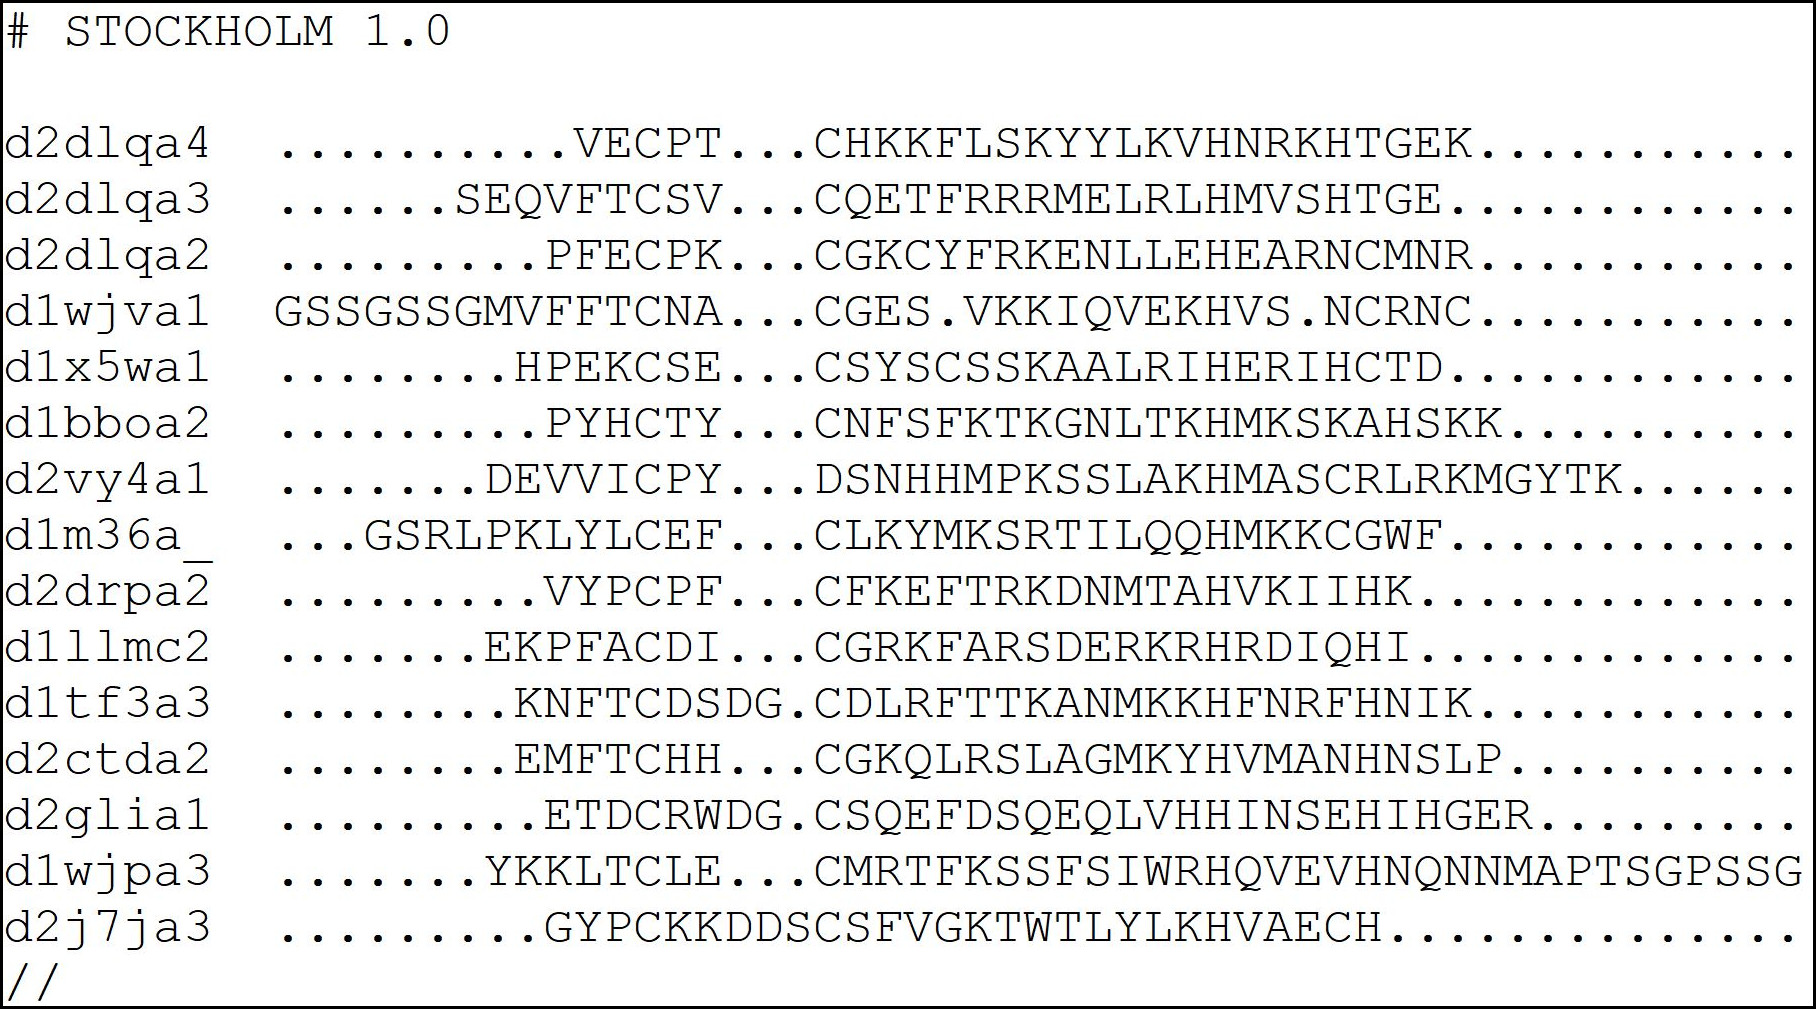
\includegraphics[width=0.8\textwidth]{fig/MSA}
	\end{center}
	\caption{Fifteen sequences from the \acs{SCOP} superfamily g.37.1 aligned to an \acs{MSA}.}
	\label{fig:MSA}
\end{figure}



There are different approaches for generating an \ac{MSA}, using either manual annotation by expert knowledge or automatic methods based on structural information on its different levels (see \cite[Chapter~6]{Durbin.1998}).


\subsection{Profile Hidden Markov Model}

A \ac{pHMM} is a stochastic  model based on Markov chains used especially in bioinformatics to model an \ac{MSA} and capture its degree of structural conservation.   Figure \ref{fig:pHMM} shows the structure of a \ac{pHMM}, which uses three different types of hidden states for each column of the \ac{MSA}. These are match state $M_k$, delete state $D_k$ and insert \mbox{state $I_k$.}

\begin{figure}[h!]
	\begin{center}
		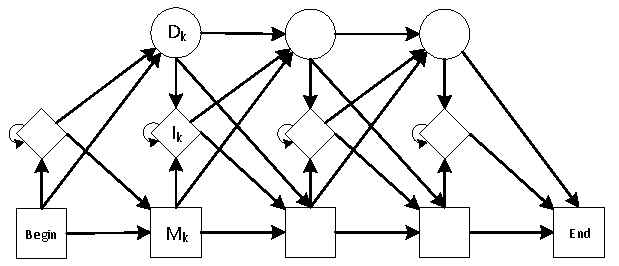
\includegraphics[width=0.85\textwidth]{fig/pHMM}
	\end{center}
	\caption[Structure of a pHMM.]{Structure of a \acs{pHMM} with match, insert and delete states, adapted from \cite{Durbin.1998}.}
	\label{fig:pHMM}
\end{figure}


Match state $M_k$ is described by a distribution, trained with the symbol frequency in column $k$ of the \ac{MSA}. Each representative column in the \ac{MSA} model matches one state. Gaps in the MSA influence the insertion and deletion states.

Insertion states model genetic insertions of additional symbols in a sequence that do not appear in the majority of the sequences of a family of proteins in the \ac{MSA}.
They occur when there are many gaps in a column, typically above 50\,\%. Insertion states  make it possible to insert the symbols in the \ac{MSA} for those sequences that do not show gaps.
Insertion states have a self-transition to cover repeated insertions over multiple columns. 
Instead of the actual symbol frequency of the \ac{MSA} column, the emission probabilities can be set to a background probability based on a general frequency of the symbols, as a few residues in the column might not be representative.

Deletions allow a sequence to skip over a match state without emitting a symbol and model situations of genetic deletions, where a certain sequence has one or more positions fewer than the other proteins in a family modeled by the \ac{MSA}.
Deletions are silent states without emitting symbol probabilities. Self-transitions are not allowed  for deletions. However, gaps over multiple columns are modeled as a sequence of deletion states, allowing different transition probabilities over multiple gap positions.


\subsection{Decoding and Scoring}
\label{sec:scoringTh}

In a fully defined \ac{pHMM}, any sequence can be represented by a matching score, by multiplying the transition and emission probabilities along the path. Due to the insert and delete states, many different paths can produce the same sequence. To find the \mbox{best-suited} path for a specific sequence, dynamic programming approaches are used, such as the \textit{forward algorithm} or the \textit{Viterbi algorithm}.

The forward algorithm calculates the overall probability as a sum for each individual state of the \ac{pHMM}. 
The Viterbi algorithm calculates the probability for the most likely sequence of states by using the maximized path over the \ac{pHMM}.

To prevent an underflow caused by the multiplication of many probabilities in the range of 0--1, a logarithmic scale is used to calculate the raw score. However, these raw scores are highly dependent on the overall sequence length, as longer sequences generate smaller scores, and thus these raw scores are difficult to compare. Therefore, the scores can be normalized using correction methods such as null models, which can either be simple null models or reversed-sequence null models. The simple null model uses a simplified one-state \ac{HMM} with a specific residue composition based on general occurrence frequencies of the amino acids and scores the sequence against it. The reversed-sequence null model uses the original \ac{pHMM} and scoring algorithm, but reverses the direction of the sequence employed. The final score without length dependency is calculated by subtracting the null model score from the raw score in the logarithmic scale.
\chapter{Protein Structure Determination}
\label{ch:PSD}

This chapter covers the fundamental methods of protein structure determination on its different levels. It begins with protein sequencing for determining the primary structure of a polypeptide. The discussion proceeds with the two major methods for determining the tertiary structure, namely \ac{XRC} and \ac{NMR}. Finally, methods for secondary structure determination are described, where the secondary structure is either derived from the tertiary structure or predicted from the primary structure.


\section{Protein Sequencing}
\label{sec:ProtSequencing}

Protein sequencing is the process of determining the primary structure of a polypeptide. Protein sequencing is the first essential step for gathering more information about the structure and function of a protein. 
Two major methods for protein sequencing are Edman degradation and mass spectrometry.

Edman degradation, developed by Pehr Edman in 1950, determines each amino acid residue through a repetitive approach, where the peptide bond of the first amino acid at the N-terminus of the peptide chain is labeled and chemically separated from the chain while keeping the remaining bonds untouched. The separated residue is identified  by procedures such as ion exchange chromatography. Ion exchange chromatography separates ionizable molecules according to differences in their total charge by increasing the ionic force of the sample medium and measuring the strength needed for each element to separate. The Edman degradation method is only reliable for short peptides up to 40--60 residues. Longer proteins must be analyzed by fragmentation, where the polypeptide is split into shorter sections and these sections are analyzed one after another \cite{Berg.imp.2002}.


Another approach is protein sequencing by mass spectrometry. Mass spectrometry uses the spectrum of a peptide to determine its sequence according to the different masses of the 20 amino acid residues. This is done by ionizing the protein molecules in a strong electric field. The ionized particles can then be detected by a mass analyzer, which provides the mass-to-charge ratio for each ion. The mass-to-charge ratio over the induced electrical energy produces a mass spectrum. The amino acid sequence can be determined from this mass spectrum by fragmentation of the molecules and also by computational analysis and matching with databases \cite{Wysocki.2005}.

With high-throughput variations of mass spectrometry such as tandem mass spectrometry or protein sequencing machines that automatically perform the process of Edman degradation, the amino acid sequence can be determined within hours \cite{Nelson.2013}.
 

\section{X-ray crystallography}

The first high-resolution three-dimensional protein structure myoglobin was identified in 1958 by
John Kendrew using \acf{XRC}, for which he received the 1962 Nobel Prize in Chemistry \cite{kendrew1958three}. Ninety percent of the determined protein structures in the PDB have been solved using \ac{XRC} \cite{Burley.2018}.  

X-ray crystallography is a form of microscopy that uses electromagnetic radiation beams.  
These beams have a wavelength of around 1\,\ac{angstrom}\footnote{\AA ngstrom (\AA) is a unit to measure the wavelength of light, 1\,\AA \, equals to $10^{-10}$\,meter or 0.1\,nanometer.}. For comparison, the inter-atomic distances of protein crystals are approximately  1--3\,\ac{angstrom}. 
The X-ray beams are diffracted by the protein's electrons when passing the crystal. The resulting diffraction pattern is collected by digital \ac{CCD} image sensors for further processing. 
Several measurements with different angles and intensities produce multiple diffraction patterns, from which a three-dimensional electron density map can be computed. The density map provides direct information about the mean positions and size of the atoms and the length and types of chemical bonds, among other aspects, which enables its primary structure to be modelled into its three-dimensional structure.

In order to obtain usable results from the protein molecules, the sample has to be purified and set in a stable crystal state. Protein molecules in their natural form are not stagnant, as there is always movement, rotation and bending in the structure. In addition, the x-ray radiation during the measurement influences the sample. A \mbox{high-quality} crystal is composed of a regular repeating arrangement of proteins, with a size in all dimensions of at least 20\,\textmu m that can extend up to and beyond 0.1\,mm. 



Protein crystallization is the crucial part of \ac{XRC} which determines whether a protein structure can be determined using this approach. There is no straightforward approach for crystallization, as each new protein may respond differently. The path from a protein to a usable crystal often involves an extensive trial and error approach, which can last months. Furthermore, some proteins do not form crystals at all, without any indication why this is the case 
\cite{McPherson.2014}. 
There are several different physical, chemical, and biochemical factors affecting the crystallization process. For example, the  earth's gravity force can prevent crystals from growing to the required size. Experiments in microgravity have in many cases improved the size and quality of protein crystals. Currently, on a regular basis, protein samples that fail to grow crystals with the required quality and size are transported to the International Space Station (ISS), where the crew continues to search for usable crystals\footnote{NASA Protein Crystals in Microgravity: \url{https://www.nasa.gov/mission_pages/station/research/benefits/mab} (accessed July 18, 2018).}. However, these experiments presuppose a certain degree of crystallization success on Earth, as the process must be highly automated and practicable for the ISS crew to be able to implement it  \cite{McPherson.2015}. 


\section{Nuclear Magnetic Resonance Spectroscopy}

\acf{NMR}, which has been used to determine 
9\,\% of protein structures in the \ac{PDB}, is the second-most-used application for identifying the \mbox{three-dimensional} structures of proteins  \cite{Burley.2018}.


This method makes use of the quantum-mechanical property of subatomic particles known as spin, which can be thought of as a rotation around the particle's own axis. Atomic nuclei with an odd number of protons and/or neutrons have spin, while nuclei with even numbers of these particles have no spin. Nuclei without spin cannot absorb or emit electromagnetic radiation, and therefore cannot be used for \ac{NMR}. However, most nuclei in proteins, such as those in the backbone ($^2$H, $^{13}$C, $^{15}$N, $^{17}$O), do have spin.

 The spinning of the nucleus generates a nuclear magnetic moment. When an external magnetic field is applied, the nucleus acts like a magnetic dipole and can orient itself in two different spin states, referred to as $\alpha$ and $\beta$. 
The $\alpha$ state is the preferred orientation in terms of energy, where the magnetic moment matches with the applied magnetic field. The orientation can be reversed to the $\beta$ state by irradiating the nucleus with an additional electromagnetic radiation frequency. The so-called resonance frequency is equal to the energy difference needed for the nucleus to switch its state and is directly proportional to the magnetic field applied.
 
By varying the frequency while maintaining a static magnetic field or vice versa, a resonance spectrum for a molecule can be obtained. The resonance spectrum indicates the energy necessary to put various nuclei in resonance. Each nucleus has its own characteristic resonance frequency, for example $^1$H with  approximately 500\,MHz and $^{13}$C with 126\,MHz. 
However, the resonance frequency of a single nucleus also varies at different locations in the molecule, due to various interactions between other subatomic particles. For example, negatively charged electrons have a so-called shielding effect, which reduces the force from the applied magnetic field that is absorbed by the nearby nuclei. 
This effect also reduces the electromagnetic radiation intensity needed to spin the nucleus  in 
 $\beta$ state.
Furthermore, the interaction from one nucleus with its surrounding nuclei can be measured by emitting frequency pulses that only bring specific nuclei in resonance. The information obtained is used to calculate the three-dimensional structure of a protein through computational analysis and molecular modeling procedures \cite{Edwards.2009}. 

An advantage of \ac{NMR} over \ac{XRC} is that the protein can be analyzed while in solution. Therefore, \ac{NMR} can be used on proteins that refuse to form crystals. 
The liquid form also provides information about the protein's stability and its dynamic processes, as the protein has freedom to move. However, the fluid state also impacts the protein's stability, as its structural integrity must be maintained over the entire experiment. The movement of the protein in solution also restricts the size of the protein, in most cases to less than  30\,kDa\footnote{Dalton (Da) is a unit to measure atomic mass, 1\,Da is equal to 1/12 the mass of a single carbon-12 atom. } or on average 250 amino acid residues \cite{Milo.2016}.
Furthermore, \mbox{high-resolution} \ac{NMR} spectrometers are relatively expensive, as the resolution is directly related to the magnetic field strength. To create the magnetic field necessary for protein structure determination, \ac{NMR} spectrometers  need expensive \mbox{liquid-helium-cooled} superconducting magnets.















\section{Secondary Structure Estimation}
\label{ssec:SSPred}

Secondary structure prediction methods rely on the annotation of known three-dimensional data, as the annotated structure serves as the training input for prediction methods. The accuracy of secondary structure prediction methods is typically measured in the percentage of correctly assigned elements for each of the three main elements, namely  $\alpha$-helix (Q$_H$), $\beta$-strand (Q$_E$) and turn (Q$_C$), and in particular the overall three-state accuracy (Q$_3$).

Early methods of secondary structure prediction, such as the \textit{Chou-Fasman method} developed in 1978, used an approach which assigns the classes $\alpha$-helix and $\beta$-strand based on statistical properties on the amino acid residues. The later \textit{GOR method} includes statistical principles based on Bayes' theorem to include the conformation probability of the chain.
While early implementations of GOR and Chou-Fasman  only reached a Q$_3$ accuracy of 50--60\,\%, the current implementation of GOR V reaches a Q$_3$ accuracy of 73.5\,\% \citep{Sen.2005}. 

Modern approaches make use of statistical methods like \acp{NN}, \acp{SVM} and \acp{HMM}. 
These methods use black-box approaches, where the path from the sequence to the structure is not obvious, due to the model being trained using machine learning.  These methods reach a Q$_3$ accuracy of > 80\,\%. With growing training data from new experimentally determined tertiary structures, this value is also increasing over time. Nevertheless, in theory the average  Q$_3$ accuracy limit for predicting secondary structure is approximately    88\,\% \cite{Rost.2003}.

In what follows, methods for determining secondary structure information will be explained. First, the secondary structure annotation method  \ac{DSSP}, which uses the tertiary structure, will be described.
Subsequently, secondary structure prediction approaches based on the primary structure will be discussed. These include the state-of-the-art methods \ac{PHD}, SPINE-X and MetaSSPred.




\subsection{The Dictionary of Secondary Structures in Proteins (DSSP)}
\label{sec:DSSP}

The \ac{DSSP}, described in \cite{Kabsch.1983}, is a method developed by Kabsch and Sander to determine the secondary structure of a protein based on the atomic coordinates of the protein. It uses pattern recognition in hydrogen bonding and specific geometric features to assign one of eight secondary structures (see Table \ref{tab:DSSPStruct})  to each residue in a protein. These eight types can be grouped into three major components: helix (H, G, I), strand (B, E) and loop (T, S, C). 


\begin{table}[h!]
	\centering
	\begin{tabular}{|c|c|l|}
		\firsthline
		 3-state SS	& DSSP	  & Secondary Structure  \\ \hline
				& H       &  $\alpha$-helix \\
			$\alpha$ (H)	& G       &  $3_{10}$ helix \\	
				& I       &  $\pi$-helix \\	\hline

				$\beta$ (E) & \begin{tabular}{@{}c@{}}B \\ E\end{tabular} &
				\begin{tabular}{@{}l@{}}residue in isolated $\beta$ bridge \\ extended strand \end{tabular} \\ \hline

				& T       &  hydrogen bounded turn \\	
		L (C) & S       &  bend \\
				& C 		&  loop or irregular \\\hline
	\end{tabular}
	\caption[Structure types determined by DSSP.]{Structure types determined by DSSP \cite{Kabsch.1983}.}
	\label{tab:DSSPStruct}
\end{table}


Hydrogen bonds are determined by approximation of the interaction energy between the $NH$ group of one amino acid and the $CO$ group of another spatially proximate amino acid. The total electrostatic energy $E$, measured in $\frac{kcal}{mol}$, is calculated according to (\ref{eq:dssp}), where $r_{AB}$ represents the inter-atomic distance of the two atoms A and B measured in \ac{angstrom}, the electron charges  $q^+ = 0.2\,e$ and $q^- = -0.42\,e$ between $NC$ and $OH$, respectively, and a dimensional factor $f = 332 \,\AA \frac{kcal}{e^2}$.

\begin{equation}
E = fq^{+} q^{-}( \frac{1}{r_{ON}} + \frac{1}{r_{CH}} - \frac{1}{r_{OH}} - \frac{1}{r_{CN}})
\label{eq:dssp}
\end{equation}

When $E < -0.5\,\frac{kcal}{mol}$, it is assumed that this position forms a hydrogen bond. After determining  all hydrogen bonds, the secondary structure is assigned by identifying the basic hydrogen binding patterns. For example, the $\alpha$-helix is identified by two consecutive hydrogen bonds between amino acid residues of the backbone that are four positions  apart. 
The $3_{10}$-helix and $\pi$-helix are variations with hydrogen bond distances of three and five residues, respectively.  
The two types of beta strands are stretched chains arranged for repeating hydrogen bonds with other strands

There are many other annotation methods to annotate secondary structure. 
For example, STRIDE uses a similar variation of hydrogen-bond patterns, but also takes into account the dihedral angles $\phi$ and $\psi$ of the protein backbone \cite{Frishman.1995}.
In contrast, DEFINE uses a  different approach, by comparing only the coordinates of the central $C_\alpha$ atoms with linear distance masks of the different ideal secondary structures \cite{Richards.1988}. 
The secondary structure outputs from these methods are not unique. By comparing the results reduced to the three major components, the two similar approaches \ac{DSSP} and STRIDE agree on 95\,\% of all positions. Including DEFINE, all three methods have only  75\,\% agreement  \cite{Cuff.1999}. 
While there are more modern and complex approaches than \ac{DSSP} available, this approach has become the standard method for most secondary structure annotation tasks. In \cite{Wilman.2014}, Wilman explains the general acceptance of \ac{DSSP} based on the simplicity of the algorithm and the availability of the code and software under the permissive non-copyleft free software license  Boost\footnote{Boost Software License: \url{https://www.boost.org/LICENSE_1_0.txt} (Accessed: July 18, 2018).}. 


\subsection{Profile Network from HeiDelberg (PHD)}


The secondary structure prediction method \acf{PHD}, introduced in \cite{Rost.1993b} by Rost and Sander, was the first method to predict secondary structure with an accuracy greater than 70\,\% from the primary structure alone.  

The \ac{PHD} method uses three steps to predict the secondary structure. %%%%%%%%%%%%%%%%%%%%%%%%%%%%%%%%%%%%%%%%%%%%%%%%%%%%%%%%%%%%
In the first step, sequences with a high sequence similarity are obtained and aligned to an \ac{MSA}. This includes additional evolutionary information, as sequences with a high sequence similarity are likely to share the same function, and thus a similar structure. %%%%%%%%%%%%%%%%%%%%%%%%%%%%%%%%%%%%%%%%%%%%%
In the second step, the probability for each amino acid in the \ac{MSA} is fed into a two-level feed-forward \ac{NN} system, previously trained through  back-propagation with proteins of known structures. 
In the first level, for each position in the sequence, a sliding window of 13 consecutive amino acids is fed. This is done with the frequency of the 20 amino acids and an additional position for padding of both ends of the sequence.
The first \ac{NN} level outputs a likelihood of the central residue being a helix, sheet, or loop.  
The independently trained second \ac{NN} level receives the output from the first level and inputs the likelihood of the three states with a sliding window of 17 elements. The second-level output is an optimized likelihood for the same three major secondary structure elements. 
The highest value for each element of the \ac{NN} determines the secondary structure. A reliability index for each residue is set with the difference between the two highest values. %%%%%%%%%%%%%%%%%%%%%%%%%%%%%%%%%%%%%%%%%%%%%%%%%%%%%%%%%%%%%%
The final step is a simple filter to remove obvious errors, like  helices shorter than three residues long.

Secondary structure prediction with \ac{PHD} is available online with the PredictProtein web server\footnote{PredictProtein web server: \url{https://www.predictprotein.org/} (Accessed July 18, 2018).} or locally through the Debian Linux package PROFPhd. The expected accuracy for the three major secondary structure types is 76\,\% on average \cite{Rost.2004}.


\subsection{SPINE-X}
\label{ssec:spinex}

Another high-accuracy secondary structure prediction method is SPINE-X  by Faraggi et al., as described in \cite{Faraggi.2012}.

In addition to the secondary structure, SPINE-X also predicts the \ac{ASA} and the  dihedral  angles $\phi$ and $\psi$ for each amino acid residue. 
The \ac{ASA} is the surface area of an amino acid that can interact with a solvent and is measured in square \AA . 
SPINE-X uses an iterative approach of six \acp{NN}, each fed with additional data predicted from the previous steps. 
Like \ac{PHD}, SPINE-X includes evolutionary information about the sequence by generating a \ac{PSSM}, which describes column-wise sequences similar to \acp{MSA}. The aligned sequences are collected by PSI-BLAST, a tool for collecting and aligning distant relatives' proteins for the query sequence (see \cite{Altschul.1998}).
Furthermore, the \acp{NN} are also individually trained with back-propagation and make use of sliding windows. 


The first \ac{NN} predicts the secondary structure by using the \ac{PSSM} generated  from the sequence and seven \acp{PP} for each amino acid residue as input. These \acp{PP} include hydrophobicity, volume, steric parameter, polarizability, isoelectric point, helix probability and sheet  probability (see section \ref{ssec:SSPred}).
The secondary structure predicted from the first step, together with the \ac{PSSM} and the \acp{PP}, is fed to the second \ac{NN} and provides the \ac{ASA} for each residue.
The third \ac{NN} uses the same properties as before and includes the \ac{ASA} in order to predict the two dihedral angles. 
The stages before the fourth step also include the output from the last step, but without the  secondary structure predicted from the first step, in order to predict an optimized version of the secondary structure.
Including the secondary structure in the input, the two dihedral angels are re-predicted in the fifth \ac{NN}. 
The sixth and final \ac{NN} predicts the final secondary structure elements, based on the \ac{PSSM}, \acp{PP} and \ac{ASA} from step two and the dihedral angles from step five.
SPINE-X predicts the secondary structure based on the eight-state \ac{DSSP} assignment. To increase accuracy, the final result is grouped into the three major types helix (H), strand (E) and coil (C) (see section \ref{ssec:backbone}).  

SPINE-X reaches a Q$_3$ accuracy of 82--83.8\,\% and is available as Linux package or online through a web server\footnote{SPINE-X web server: \url{http://sparks-lab.org/SPINE-X/} (Accessed July 18, 2018).}.


\subsection{MetaSSPred}
\label{sec:BSSP}

MetaSSPred is a secondary structure prediction method, developed in the Bioinformatics and Machine Learning Lab\footnote{Bioinformatics \& Machine Learning Lab UNO: \url{http://biomall.cs.uno.edu/} (accessed July 18, 2018).} at the University of New Orleans (see \cite{NasrulIslam.2016}). 

MetaSSPred uses three binary \acp{SVM}, together also referred as cSVM, to predict the secondary structure, then combines its results with SPINE-X to improve the accuracy, especially for $\beta$-sheets. 
While modern secondary structure prediction methods reach an average Q$_3$ accuracy of more than 80\,\%, the accuracy of each type varies greatly. In particular, $\beta$-sheet scores are likely to be far below the others. For example, while SPINE-X reaches a Q$_3$ accuracy of 82\,\%, helices are correctly predicted with a Q$_H$ of 86.6\,\%, coils with a Q$_C$ of 81.5\,\%, and sheets with a Q$_E$ of 75.3\,\% \cite{Faraggi.2012}.

The \acp{SVM} are trained by 33 features for each amino acid listed in Table \ref{tab:MetaPred}. These features are assigned directly by the primary structure or gathered by the tools described below.  
For each amino acid residue, the seven \acp{PP} as described in Section \ref{ssec:ppaa} are used. The terminal indicator marks whether the residue is one of the first or last five residues in the sequence. As in the case of SPINE-X, the \ac{PSSM} is determined by PSI-BLAST. The disorder probability is the probability that an amino acid residue in the chain does not have a well-defined three-dimensional structure and can thus arrange in several other conformations. The disorder probability is predicted by the application DisPredict (see \cite{Iqbal.2015}). 
The two dihedral angles $\phi$ and $\psi$ are predicted by SPINE-X (see Section \ref{ssec:spinex}).
While \ac{ASA} could also be taken from the SPINE-X prediction, the application REGAd$^3$p with its higher prediction accuracy is used \cite{Iqbal.2015_2}.

\begin{table}[h]
\centering
\begin{tabular}{|l|c|r|} \hline
Feature                          & Count & Method           \\ \hline
Amino acid (AA)                      & 1	 &    Primary Structure				\\
\acf{PP}        & 7     &          Primary Structure           				\\
Terminal indicator               & 1     &    Primary Structure          	\\  
\acf{PSSM} & 20    &  PSI-BLAST       \\	  
Disorder probability             & 1     &  DisPredict      \\
Torsion angles ($\psi$, $\psi$) fluctuation       & 2     &  SPINE-X  \\
\acf{ASA}          & 1     &  REGAd$^3$p    		\\ \hline
\end{tabular}
\caption[The 33 features used by MetaSSPred.]{The 33 features used by MetaSSPred with the methods to determine them from the primary structure \cite{NasrulIslam.2016}.}
\label{tab:MetaPred}
\end{table}

For one of the three secondary structure classes, each \ac{SVM} predicts whether a residue belongs to the secondary structure class and returns a probability that this is the case. 
For each residue in the sequence, the secondary structure element with the highest probability is assigned. 
In the final step, the output from cSVM is combined with the prediction from SPINE-X. For each residue, the predicted secondary structure class is compared. 
For all positions of cSVM where the class sheet (E) is predicted, 
the result from cSVM will be accepted if it belongs to the class sheet, otherwise the predicted class from SPINE-X is used. 
MetaSSPred is available as a Linux-based standalone software package\footnote{MetaSSPred package: \url{http://biomall.cs.uno.edu/software/} (accessed July 18, 2018).}.


\chapter{Implementation}
\label{ch:implement}

This chapter covers the implementation based on the HMModelers workflow. First, the processing of input data by including secondary structure data is described. This is followed by a description of the adaptation of the \ac{pHMM} and of the scoring algorithms. This section focuses on the modifications made in HMModeler. More information on HMModeler and its other implementations can be found in \cite{Graf.2011, MathiasOberkirchner.2014, Mayer.2014}.

\section{HMModeler}

HMModeler is a software package for protein classification jointly developed by researchers at the Salzburg University of Applied Sciences and the University of Salzburg. 
Although HMModeler was designed as an extension for UCSF Chimera\footnote{UCSF Chimera \url{https://www.cgl.ucsf.edu/chimera/} (accessed July 18, 2018).}, the current version runs independently with its own \ac{GUI}. The core of HMModeler is written in Python, while time-consuming algorithms are also implemented with faster C++ libraries. The  web-based \ac{GUI} communicates with the core system via RESTful\footnote{Representational State Transfer (REST) is an architectural paradigm for communication between distributed machines or applications.} web services. HMModeler is platform-independent and runs both on Windows and Linux operating systems. 
The program uses the Smith-Watermann-style variant of \ac{pHMM}, shown in Figure \ref{fig:pHHMsw}. This variant is used for local alignments, by using flanking states with transitions from the beginning to each match state as start-model, and from each match state to the end state as end-model. 

The \ac{GUI} allows skilled experts to introduce prior information about the targeted protein family into the \ac{HMM}. In particular, the user can interactively define parts of the protein with increased or decreased insertion and deletion probabilities. The user can also modify the extent to which the emission probabilities in the single-model columns of the \ac{pHMM} are extracted. This can be done purely through the given \ac{MSA}; alternatively, the probabilities are determined from a priori distributions.
Finally, the user can define so-called expert sets that override other estimation methods and set the possible emissions in certain model states to an explicit set of amino acids. Currently, the software only uses the primary structure for building the \ac{pHMM} and scores sequences against it with the Viterbi and forward algorithms.
 



\begin{figure}[H]
	\begin{center}
		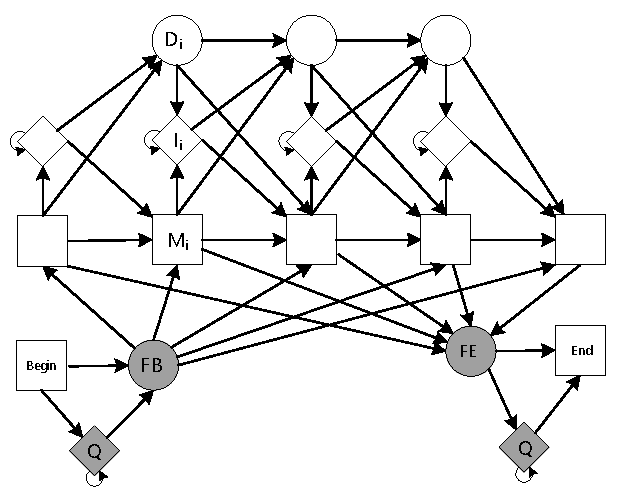
\includegraphics[width=0.78\textwidth]{fig/pHMMsw}
	\end{center}
	\caption[Smith-Waterman variant of a \acs{pHMM}.]{Smith-Waterman variant of a \acs{pHMM}, adapted from \cite{Durbin.1998}.}
	\label{fig:pHHMsw}
\end{figure}

\section{Input Data}
\label{sec:inputData}

First, HMModeler takes an \ac{MSA} as input to train its \ac{pHMM}. HMModeler can process files in the \textit{Stockholm} file format, uploaded by the user or referenced by a project ID from the multiple structure alignment Server PIRATES\footnote{Multiple structure alignment server PIRATES: \url{https://biwww.che.sbg.ac.at/pirates} (accessed July 18, 2018).}. 

The Stockholm format is a markup format for \ac{MSA}, where each sequence can be annotated with additional features, such as the corresponding secondary structure for each amino acid residue. The definition of the Stockholm format can be found in \cite{Sonnhammer.xxx}. 

Figure \ref{fig:flowReadMSA} shows the workflow implemented for determining the secondary structure. First, all sequences in the \ac{MSA} are read. 
If no structure information is provided for one or more sequences, the secondary structure is retrieved from the \ac{PDB} or predicted using the MetaSSPred method (see Section \ref{sec:BSSP}).

\begin{figure}[ht]
	\begin{center}
		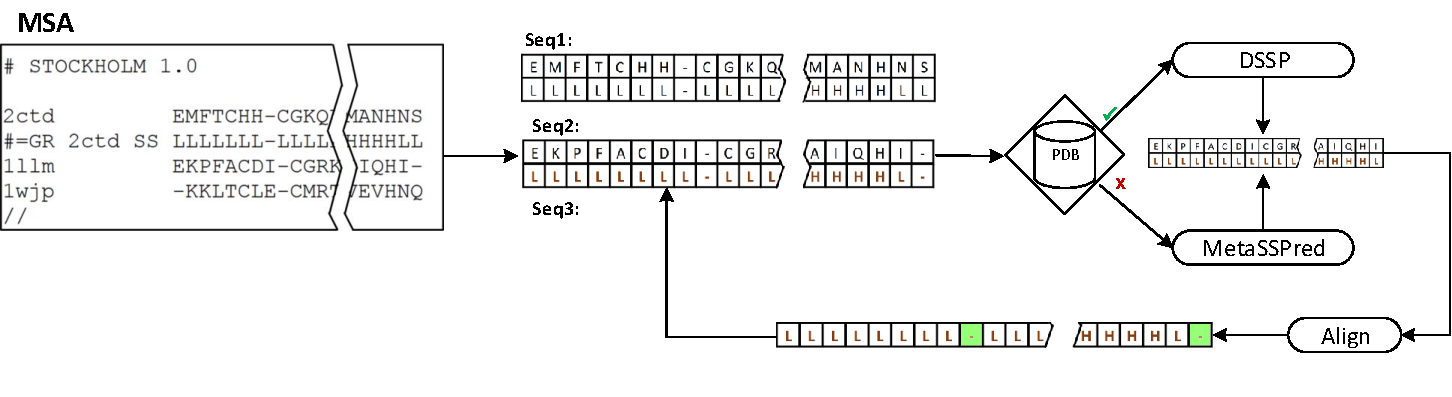
\includegraphics[width=\textwidth]{fig/ablaufMSA}
	\end{center}
	\caption[Workflow for processing input data.]{Workflow for processing input data and determination of secondary structure.}
	\label{fig:flowReadMSA}
\end{figure}

The secondary structure from sequences corresponding to three-dimensional data in the \ac{PDB} is calculated using the \ac{DSSP} program (see Section \ref{sec:DSSP}). The extracted structural information must be aligned with the original sequence, considering the exact gap positions and possible differences in the overall sequence length.  
The \mbox{Needleman--Wunsch} algorithm, described in \cite[p.\,19--21]{Durbin.1998}, is used for this task. 
Needleman--Wunsch is a dynamic programming approach for global sequence alignment that calculates the optimal path through a scoring matrix using match, mismatch, and gap penalties.
The derived sequences, linked to their corresponding secondary structure, are aligned with the original sequence. Provided the original sequence from the \ac{MSA} matches the aligned sequence from the \ac{PDB}, the determined secondary structure is used. 

If there is no match in the \ac{PDB} or the alignment fails, the secondary structure is predicted with MetaSSPred. For each sequence that must be predicted, a Fasta-formatted file with all gaps removed in the sequence is generated in the input directory of MetaSSPred and processed by the software. For the prediction process, ambiguous amino acids have to be treated separately, as most prediction methods including MetaSSPred only support the 20 common amino acids. Therefore, those symbols are also  removed for the prediction process. 
Subsequently, the symbol X is added at the removed position in the secondary structure data, which will be handled by HMModeler in the same way as all three secondary structure types.
Finally, the predicted secondary structure is aligned to the sequence with the Needleman--Wunsch algorithm. 

\section{Training the HMM}
\label{sec:training}

Based on the \ac{MSA}, which now includes both primary and secondary structures, the transitions and emission distribution are assigned to the \ac{pHMM}.
These are calculated by the frequencies across sequences for each column in the \ac{MSA}, according to (\ref{eq:transProb}), where $a_{kl}$ is the transition probability from state $k$ to $l$, and (\ref{eq:emission}) for the emission probability $e_k(a)$ of the symbol $a$ at state $k$. 

\begin{equation}
a_{kl} = \frac{A_{kl}}{\sum_{l'}A_{kl'}}
\label{eq:transProb}
\end{equation}

\begin{equation}
e_{k}(a) = \frac{E_k(a)}{\sum_{a'}E_k(a')}
\label{eq:emission}
\end{equation}

To prevent overfitting by symbols with a probability of zero, it is important to add some background frequency to each symbol, such as a small non-zero prior probability $pc(a)$ (see (\ref{eq:pseudo})). The simplest approach is the Laplace smoother, which adds a hypothetical observation in the form of one pseudo-count to each emission and transition.

\begin{equation}
e_{k}(a) = \frac{E_k(a) + pc(a)}{\sum_{a'}E_k(a') + \sum pc(a')}
\label{eq:pseudo}
\end{equation}


The implementation for the emission probabilities was extended by calculating the primary structure with 20+1 symbols to generate two additional matrices, one with 3+1 symbols for the secondary structure and another with 84 symbols containing mixed probabilities from the other two sets. The additional symbol for the primary and secondary structures was added to cover a wider set of sequences in the test database (see Section \ref{sec:TestData}), where single residues or structure elements in sequences may be unknown and therefore marked with the letter X. As the symbol X represents all other symbols in the set, the probability is set to 1. This is equal to the sum of all other probabilities. 


The transition probabilities only rely  on the gap positions of the \ac{MSA}. Therefore, no modifications in the current implementation of HMModeler are needed. Moreover, the functional emission probability implementation for the primary structure remains the same.

The emission probabilities for the secondary structure are calculated by using the three major types of helix, strand and loop. Therefore, secondary structure data from methods with higher granularity, such as \ac{DSSP}, are translated to the three-type annotation (see Table \ref{tab:DSSPStruct}). 
  To prevent zero probabilities, a prior probability can be set by the user in the HMModeler \ac{GUI}.

Using both probability sets, the original primary structure implementation and the new secondary structure probabilities, a weighted emission frequency set that covers both primary and secondary probabilities is generated. 
Mayer discusses the emission probability weighting for use with \ac{pHMM} in \cite{Mayer.2014}. Following his research, three different implementations are explained below.

\subsection{Linear Weighting}

In \cite{Mayer.2014}, Mayer discusses the problem with the different length of the two alphabets, as the primary structures involve 20 amino acid symbols and the secondary structure only involves three symbols. Therefore, he recommends  the approach in  (\ref{eq:mix1}), where the mixed emission probabilities $e_k(p,s)$ are weighted by their symbol length with 20 amino acids for the primary probability $e_k(p)$ and the three structure symbols in $e_k(s)$.   

\begin{equation}
e_k(p,s) = \frac{20}{20+3}\cdot e_k(p) + \frac{3}{20+3} \cdot e_k (s)
\label{eq:mix1}
\end{equation}


However, the most convenient approach for mixing two probabilities, which is by means of a simple multiplication as in  (\ref{eq:mix2}), will also be implemented and tested. 

\begin{equation}
e_k(p,s) =  e_k(p) \cdot e_k (s) \cdot k
\label{eq:mix2}
\end{equation}

As mentioned in Section \ref{sec:scoring} below, a threshold can be used to define whether  the scoring process uses the mixed or the primary  probability. The additional factor $k$ is introduced for scaling the resulting mixed probability. 
With this factor, the differences in the \ac{pHMM} resulting from the use of either mixed probability or primary probability can be reduced.


For example, if the three secondary structure elements are equally distributed with a probability of $e_k(s) = \frac{1}{3}$ and a $k=1$, the value of the mixed probability would also be $\frac{1}{3}$ of the value of the primary probability. By setting the factor $k=3$, an equally distributed secondary structure would not differ if the primary probability or the mixed probability were used.  

\subsection{Weighting by Shannon}


In \cite{Mayer.2014}, Mayer introduces weighting the two emission probabilities by the amount of information in each column using the Shannon theorem, defined in \cite{Shannon.1948} as 


\begin{equation}
	H = -\sum _{i=1}^{N} p_i \log _b p_i
	\label{eq:shannon1}
\end{equation}


where the entropy $H$ is the negative sum over the probability of each possible outcome $p_i$ multiplied by the logarithm of the same probability.
If a single probabilistic result of an event has a probability of $1$, the entropy is $0$. In this case, there is no uncertainty. Conversely, if all probabilistic results have equal probability, the uncertainty is maximal, with an entropy of $\log_b(N)$, where $N$ is the number of possible outcomes.  
The logarithmic base $b$ is usually $2$, as the common use is digital communication. In other cases, the natural logarithm $e$ is used. 

Figure \ref{fig:shannon} shows the entropy as a function for a binary event with probabilities $p$ and $q = 1-p$ with a natural logarithm and logarithmic base of 2. The maximum entropy occurs when $p=q=0.5$. 

\begin{figure}[ht]
	\begin{center}
		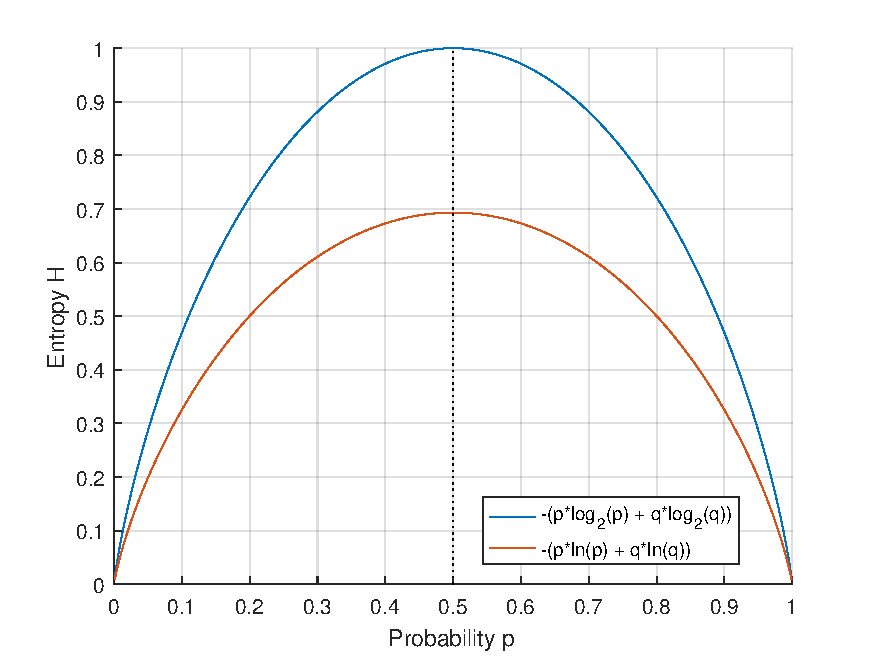
\includegraphics[width=0.8\textwidth]{fig/shannon}
	\end{center}
	\caption[Entropy H for an event with two possible outcomes.]{Entropy H for an event with two possible outcomes, with natural logarithm (red) and normalized logarithm with base 2 (blue).} 
	\label{fig:shannon}
\end{figure}


The lower the entropy, the higher the degree of information and thus the relevance of the mixed probability. The rate of information $I$ is determined by subtracting the entropy $H$ from the maximal possible entropy  $\log_b(N)$:

\begin{equation}
	I = \log_b(N)- H
\end{equation}

With the degree of information for both the primary structure $I(p)$ and the secondary structure $I(s)$, the  probabilities are weighted as follows:

\begin{equation}
	e_k(p,s) = \frac{I(p) \cdot e_k(p) + I(s) \cdot e_k(s)}{I(p)+I(s)}
	\label{eq:shannonfinal}
\end{equation}
 

Instead of using the natural logarithm for both the primary and secondary structure, as recommended by Mayer, the normalized logarithm with a base equal to the corresponding alphabet size is used in the present thesis. Without the normalization, the probabilities would not be equally weighted, as the maximum entropy for the  primary structure would be $ln(20)= 2.9957$ and for the secondary structure  $ ln(3) = 1.0986$. By contrast, the maximum entropy for both structures using the normalized logarithm is $\log_{3}(3)= \log_{20}(20) = 1$.

For programming languages that do not support nonstandard logarithmic bases, any logarithmic equation with base $a$ can be converted to any other base $b$ by dividing through the logarithm with the same base $a$, with the argument set to the new base $b$:


\begin{equation}
	\log_b(x) = \frac{\log_a(x)}{\log_a(b)}
	\label{eq:logBase}
\end{equation}
 
 
% #################################################################
%%---------------------------   SCORING     -----------------------
% #################################################################
\section{Scoring Sequences}
\label{sec:scoring}

HMModeler calculates nine different types of scores, (see Table \ref{tab:Hmscores}) using the Viterbi and forward algorithms. It also computes variations of these for length-corrected scores using the simple null model and the reversed sequence null model (see Section \ref{sec:scoringTh}). 

\begin{table}[h!]
\centering
\begin{tabular}{|l|l|}
\hline
Score type					& Description\\ \hline
Viterbi score                    & $\text{V}(s)$                         \\ 
Forward score                    & $\text{F}(s)$                         \\ 
Simple null model                & $\text{N}(s)$                         \\ 
Reverse Viterbi null model       & $\text{V}(s^{-1})$      \\ 
Reverse forward null model       & $\text{F}(s^{-1})$      \\ 
Simple corrected Viterbi score   & $\text{V}(s)-\text{N}(s)$                    \\ 
Simple corrected forward score   & $\text{F}(s)-\text{N}(s)$                    \\ 
Reverse corrected  Viterbi score & $\text{V}(s)-\text{V}(s^{-1})$ \\ 
Reverse corrected forward score \qquad & $\text{F}(s)-\text{F}(s^{-1})$   \qquad \\  \hline
\end{tabular}
\caption{Scores calculated by HMModeler.}
\label{tab:Hmscores}
\end{table}

Only the algorithms for the Viterbi score and the forward score must be adapted for the use of the secondary structure. The reversed null models for both the Viterbi and forward scores use the same underlying algorithm but with the sequence reversed. The simple null model uses a one-state \ac{HMM} with general background distribution based on the primary structure that  will continue to be used.


As described in Section \ref{sec:training}, the mixed emission probabilities $e_k(p,s)$ are generated based on the primary structure probabilities $e_k(p)$ and secondary structure probabilities $e_k(s)$. However, with the aim of using only the primary structure instead of the mixed probabilities for regions in the \ac{MSA} where the primary structure is highly conserved, a threshold can be set. If the highest emission probability in the primary structure is set below the threshold, the mixed probabilities are used. Otherwise, only the probabilities for the primary structure are used: 

\begin{equation}
e_k(m) =
  \begin{cases}
    e_k(p)  &  \text{if}\: \max(e_k(p')) > threshold \\
    e_k(p,s) & \text{otherwise}
  \end{cases}
  \label{eq:weighting}
\end{equation}

The resulting probability $e_k(m)$ will be used in the Viterbi equation for the transition to the match-state $V_j^M$:

\begin{equation}
V_k^M(k) = \log e_k(m)+ \text{max} 
\begin{cases}
V_{k-1}^M(i-1) + \log a_{M_{k-1} M_k}\\
V_{k-1}^I(i-1) + \log a_{I_{k-1} M_k}\\
V_{k-1}^D(i -1) + \log a_{D_{k-1} M_k} \\
V_{k-1}^{FB}{(i-1)} + \log a_{FB M_k}
\end{cases}
\label{eq:Viterbi}
\end{equation} 

The other Viterbi equations remain unchanged; as for insertion states in (\ref{eq:ViterbiInsert}), a background probability $q(p)$ based on the primary structure alphabet will be emitted, and the silent deletion states in (\ref{eq:ViterbiDeletion}) do not emit any symbol.

\begin{equation}
V_k^I(k) = \log q(p)+ \text{max} 
\begin{cases}
V_{k}^M(i-1) + \log a_{M_{k} D_k}\\
V_{k}^I(i-1) + \log a_{I_{k} D_k}\\
V_{k}^D(i-1) + \log a_{D_{k} D_k}
\end{cases}
\label{eq:ViterbiInsert}
\end{equation} 


\begin{equation}
V_k^D(k) = \text{max} \begin{cases}
V_{k-1}^M(i-1) + \log a_{M_{k-1} D_k}\\
V_{k-1}^I(i-1) + \log a_{I_{k-1} D_k}\\
V_{k-1}^D(i -1) + \log a_{D_{k-1} D_k} 
\end{cases}
\label{eq:ViterbiDeletion}
\end{equation} 


The same modification applies to the match state in the forward algorithm in (\ref{eq:ForwardMatch}), which is similar to the Viterbi algorithm. An exception is that instead of using the path with the maximum transition state, it sums up all transition states. 

\begin{equation}
\label{eq:ForwardMatch}
\begin{split}
F^M_k(i)= \log e_k(m) + \log&[  a_{M_{k-1}M_k} \: \exp(F_{k-1}^M(i-1))  \\
					 	  &+ a_{I_{k-1}M_k} \: \exp(F_{k-1}^I(i-1))		\\			 	  
					 	  &+ a_{D_{k-1}M_k} \: \exp(F_{k-1}^D(i-1))	\\
					 	  &+a_{FBM_k} \: \exp(F_{k-1}^{FB}(i-1))]
\end{split}
\end{equation}



\chapter{Tests and Results}
\label{ch:evaluate}

In the previous chapter, the implementation of the secondary structure logic in HMModeler was described. In the following chapter, the changes made to HMModeler will be evaluated by testing the different scoring and weighting methods that were used.

All test datasets and the database, as well as the generated scores and plots mentioned in the following chapter, can be found on the attached disk (see Appendix \ref{app:AppDisk}).

\section{Test Dataset}
\label{sec:TestData}


 The ASTRAL SCOP 1.73 sequence database\footnote{Astral SCOP 1.73: \url{https://scop.berkeley.edu/astral/ver=1.73} (accessed July 18, 2018).}, filtered to retain entries  with less than 40\,\% sequence similarity to each other, was used. This specific version was chosen because it was the latest complete manually curated version available at the time of writing this thesis.  
 The database contains 9,536 sequences with an average sequence length of 178 residues. While most residues in the database are from the 20 common amino acids listed in Table \ref{tab:AAlist}, 452 are ambiguous residues. Apart from one, these ambiguous residues are all defined as \textit{any of the 20 common amino acid residues} and represented by the letter X. 
 As described in Section \ref{sec:inputData}, the logic for sequences with the symbol X is implemented for both the primary and secondary structure. The single additional ambiguous residue, marked by the symbol Z, occurs in the sequence with the \ac{SID} \texttt{d4cpai\_}, representing a position with either glutamine (Q) or glutamic acid (E).  This sequence was removed from the database, as these rare special cases would lead to an extensive expansion of the implementation, such as an additional emission case for each possible ambiguous amino acid. Furthermore, this would also lead to an increased \mbox{run-time} of the training and scoring algorithms.  
 Another approach to handle ambiguous amino acids is, as described in \mbox{\cite[p.~183]{Baldi.2001}}, ``the  `benefit of the doubt'    approach'', where ambiguous amino acids are replaced with the most likely candidates for these positions.  
 With the sequence containing the symbol Z removed from the database, the test set finally contained 9,535 sequences. As each entry listed in \ac{SCOP} is linked to \mbox{three-dimensional} structure information in the \ac{PDB}, the secondary structure for the test set was determined using DSSP.  
 
A set of 69 \acp{MSA} based on the  same ASTRAL \ac{SCOP} 1.73 database was provided by the Department of Molecular Biology at the University of Salzburg\footnote{University of Salzburg: Department of Molecular Biology: \url{https://biwww.che.sbg.ac.at/} (accessed July 18, 2018).}. Each MSA is built up from 15 homologous sequences within  the same superfamily. 
For the first tests of the scoring and weighting methods of the \ac{pHMM}, the secondary structure from \ac{DSSP} was also used for the \ac{MSA}, as it represents the perfect condition in combination with the used test database assigned the same way. 

For the first part of the following section, the \ac{MSA} representing the \ac{SCOP} superfamily \texttt{c.67.1} will mainly be used in order to show changes in the score types when including secondary structure. 
The superfamily \texttt{c.67.1} is from the class \textit{alpha and beta proteins (a/b)} and represents \textit{pyridoxal phosphate-dependent transferase} proteins that are involved in the biosynthesis of amino acids dependent on \textit{pyridoxal phosphate}. This is the active form of vitamin B6.  
The \ac{MSA} with 15 sequences is 501 columns long. The \acp{pHMM} trained from the \ac{MSA} have a length of 384 match-states. 
More than 50\,\% of the remaining 116 columns consist of gaps and thus are represented as insertion states in the \ac{pHMM}. 
In total, the \ac{MSA} includes 5,966 residues and 1,549 gap positions.
The complete \ac{MSA} \texttt{c.67.1} in its Stockholm format is provided in Appendix \ref{app:MSAc671}. 
In the SCOP database that was used, 60 out of the 9,535 sequences are classified as belonging to the superfamily \texttt{c.67.1}.

The secondary structure for the 15 sequences of the \ac{MSA} was assigned by DSSP, using the associated structure files in the \ac{PDB}. 
The class \textit{alpha and beta proteins (a/b)}, to which the \ac{MSA} belongs, is structurally composed of alternating alpha helices and beta sheets in which the beta sheets are mostly parallel to each other. Therefore,  the \ac{MSA} is represented by a balanced number of all three secondary structure elements.
Table \ref{tab:SSdist} lists the number of occurrences and the percentage distribution of the secondary structure classes assigned by \ac{DSSP}  for the  database that was used and the \ac{MSA} \texttt{c.67.1}. The data show that in general, loops are the most common structure with 43.1\,\%, followed by helices, and finally sheets, which are the least common. 

\begin{table}[h]
\centering
\begin{tabular}{|l|rr|rr|} 
\hline
SS-Class 		& 	& SCOP 1.73			&  	& \ac{MSA} c.67.1 \\ \hline
Helix H 		& 35.1\,\%	& 594,399 		& 41.9\,\% 	& 2,497   \\
Sheet E 		& 21.8\,\%	& 368,469 		& 16.6\,\%	& 991    \\ 
Loop \,C 		& 43.1\,\%	& 729,494 		& 41.4\,\%	& 2,472   \\
Any \ \ X 		& $<0.1$\,\%	& 451    		& 0.1\,\%	& 6     	\\ \hline
Total 	&100 \% 	& \qquad 1,692,815 	& 100  \%	& \qquad 5.966 \\ \hline 
\end{tabular}
\caption[Distribution of the secondary structure elements.]{Distribution of the secondary structure elements $H$, $E$,  $C$ and $X$ in the SCOP database and the \acs{MSA} c.67.1.}
\label{tab:SSdist}
\end{table}











\section{Changes in Scores Following the Inclusion of Secondary Structure}
\label{ssec:Scores_Changes}

Initially, for all nine scores, the original scores obtained using only the primary structure and the new scores produced with secondary structure information were compared.  An overview of all 69 scores will be given in Section \ref{sec:weightingMeth}.  This section focuses on the \ac{MSA} \texttt{c.67.1} to highlight the impact of the secondary structure information on the scores. The method and parameters for the scores calculated using secondary structure is \mbox{\texttt{M2\_025\_1\_3}}. The exact configuration will be described in Section \ref{sec:weightingMeth}. 

The \ac{pHMM} was trained with the \ac{MSA} and scored against the database first with primary structure information only and then with both primary and secondary structure information. Table \ref{tab:LST_Scores} lists the average changes between the two methods' scores across all scores from the database. The changes are separated into the superfamily \texttt{c.67.1} and the other scores.

\begin{table}[h!]
	\centering
\begin{tabular}{|llr|}
\hline
Method & Family & Average score-change \\ \hline

Viterbi score				& Superfamily: \qquad & +72.7664 \\  
    						& Other:       & +21.8893 \\ \hline
Forward score 				& Superfamily:\qquad & +71.0713 \\ 
   	 						& Other:       & +25.1106 \\ \hline
Simple null score 			& Both: 		& 0 \\ \hline
Reversed Viterbi 			& Superfamily: & +53.9577 \\ 
    						& Other:       & +21.3254 \\ \hline
Reversed forward  			& Superfamily: & +64.7312 \\ 
    						& Other:       & +24.6887 \\ \hline
Simple corrected Viterbi	& Superfamily: & +72.7664 \\ 
    						& Other:       & +21.8893 \\ \hline
Simple corrected forward	& Superfamily: & +71.0713  \\ 
    						& Other:       & +25.1106 \\ \hline
Reverse corrected Viterbi	& Superfamily: & +18.8087 \\ 
    						& Other:       & +0.5639 \\ \hline
Reverse corrected forward \qquad	& Superfamily: & +6.3401 \\ 
    						& Other:       & +0.4219 \\ \hline
\end{tabular}
	\caption[Average change for \acs{MSA} c.67.1 scored against the SCOP database.]{Average change for \acs{MSA} c.67.1 scored against the SCOP database using primary structure only to including secondary structure.}
	\label{tab:LST_Scores}
\end{table}

The first two scoring methods, the plain Viterbi and forward scores, have an average increase three times higher than that of the other scores. The score for the simple null score is unchanged, as it uses a one-state \ac{HMM} with a general background distribution. As there is no change in the simple null model, the average change for both \mbox{simple-corrected} scores is the same as the plain scores. The difference between the superfamily and other scores for the reversed scores is lower than for the plain scores, while the difference for the other scores stays within decimal range. This difference between the plain and reversed scores results in an improvement of the reverse-corrected score. On average, the superfamily scores compared to the others increase by a factor of 33 for the Viterbi method and a factor of 15 for the forward method. Although this increase is an indication of a general improvement, these scores must be investigated in more detail, as there are several uncertain factors, such as the different sample sizes between the 60 superfamily scores compared to the remaining 9,475 other scores. The changes in these scores are investigated in detail in the following figures.


%%%%%%%%%%%%%%%% %%%%%%%%%%%%%%%%%%%%%%%%%%%%%%
%%%%%%%%%%%%%  FIGURE 1   %%%%%%%%%%%%%%%%%%%%%
%%%%%%%%%%%%%%%%%%%%%%%%%%%%%%%%%%%%%%%%%%%%%%%


Figure \ref{fig:eval1} shows the change in the scores for the plain and reversed scoring methods generated by HMModeler. A scatterplot is used to visualize the variation for each sequence, with the score using the secondary structure on the horizontal axis. On the vertical axis, the difference between the same score and the original score without secondary structure information is displayed. The scores in the database from sequences in the same superfamily (e.g. the \ac{MSA} used to build the \ac{pHMM}) are shown as red circles. All other scores are represented by blue circles.
The left plots show the scores related to the Viterbi scoring method and the right plots show the forward method scores. 

%%%%%%%%%%%%%%%%
%%%%%  OBEREN FIGURES
%%%%%%%%%%%%%%%
The upper plots represent the plain Viterbi and forward scores. 
They show that all scores increase, both those from the target superfamily and all the other scores.
However, the rise in the superfamily scores is noticeably higher than the rise in the other scores. 
Moreover, the higher the original scores from sequences that are not from the superfamily, the smaller the difference that results from using the secondary structure. This implies that using secondary structure information improves the plain scores significantly. However, there are still a considerable number of scores from other superfamilies that are higher than the scores of the tested superfamily. These higher-scored sequences are mainly sequences with a low residue count, as the plain scores are strongly influenced by the sequence length. The reversed scores are used to compensate for the sequence length of the plain scores, by subtracting the reversed scores from the plain scores. It is expected that the difference from the other scores will remain in the range of the plain scores above, whereas the difference for the superfamily scores should be reduced. This behavior can be observed in the two lower plots of Figure \ref{fig:eval1}, which show the scores for the reverse Viterbi (left) and the reverse forward (right). 

\begin{figure}[H]	% [b!]
	\begin{center}
		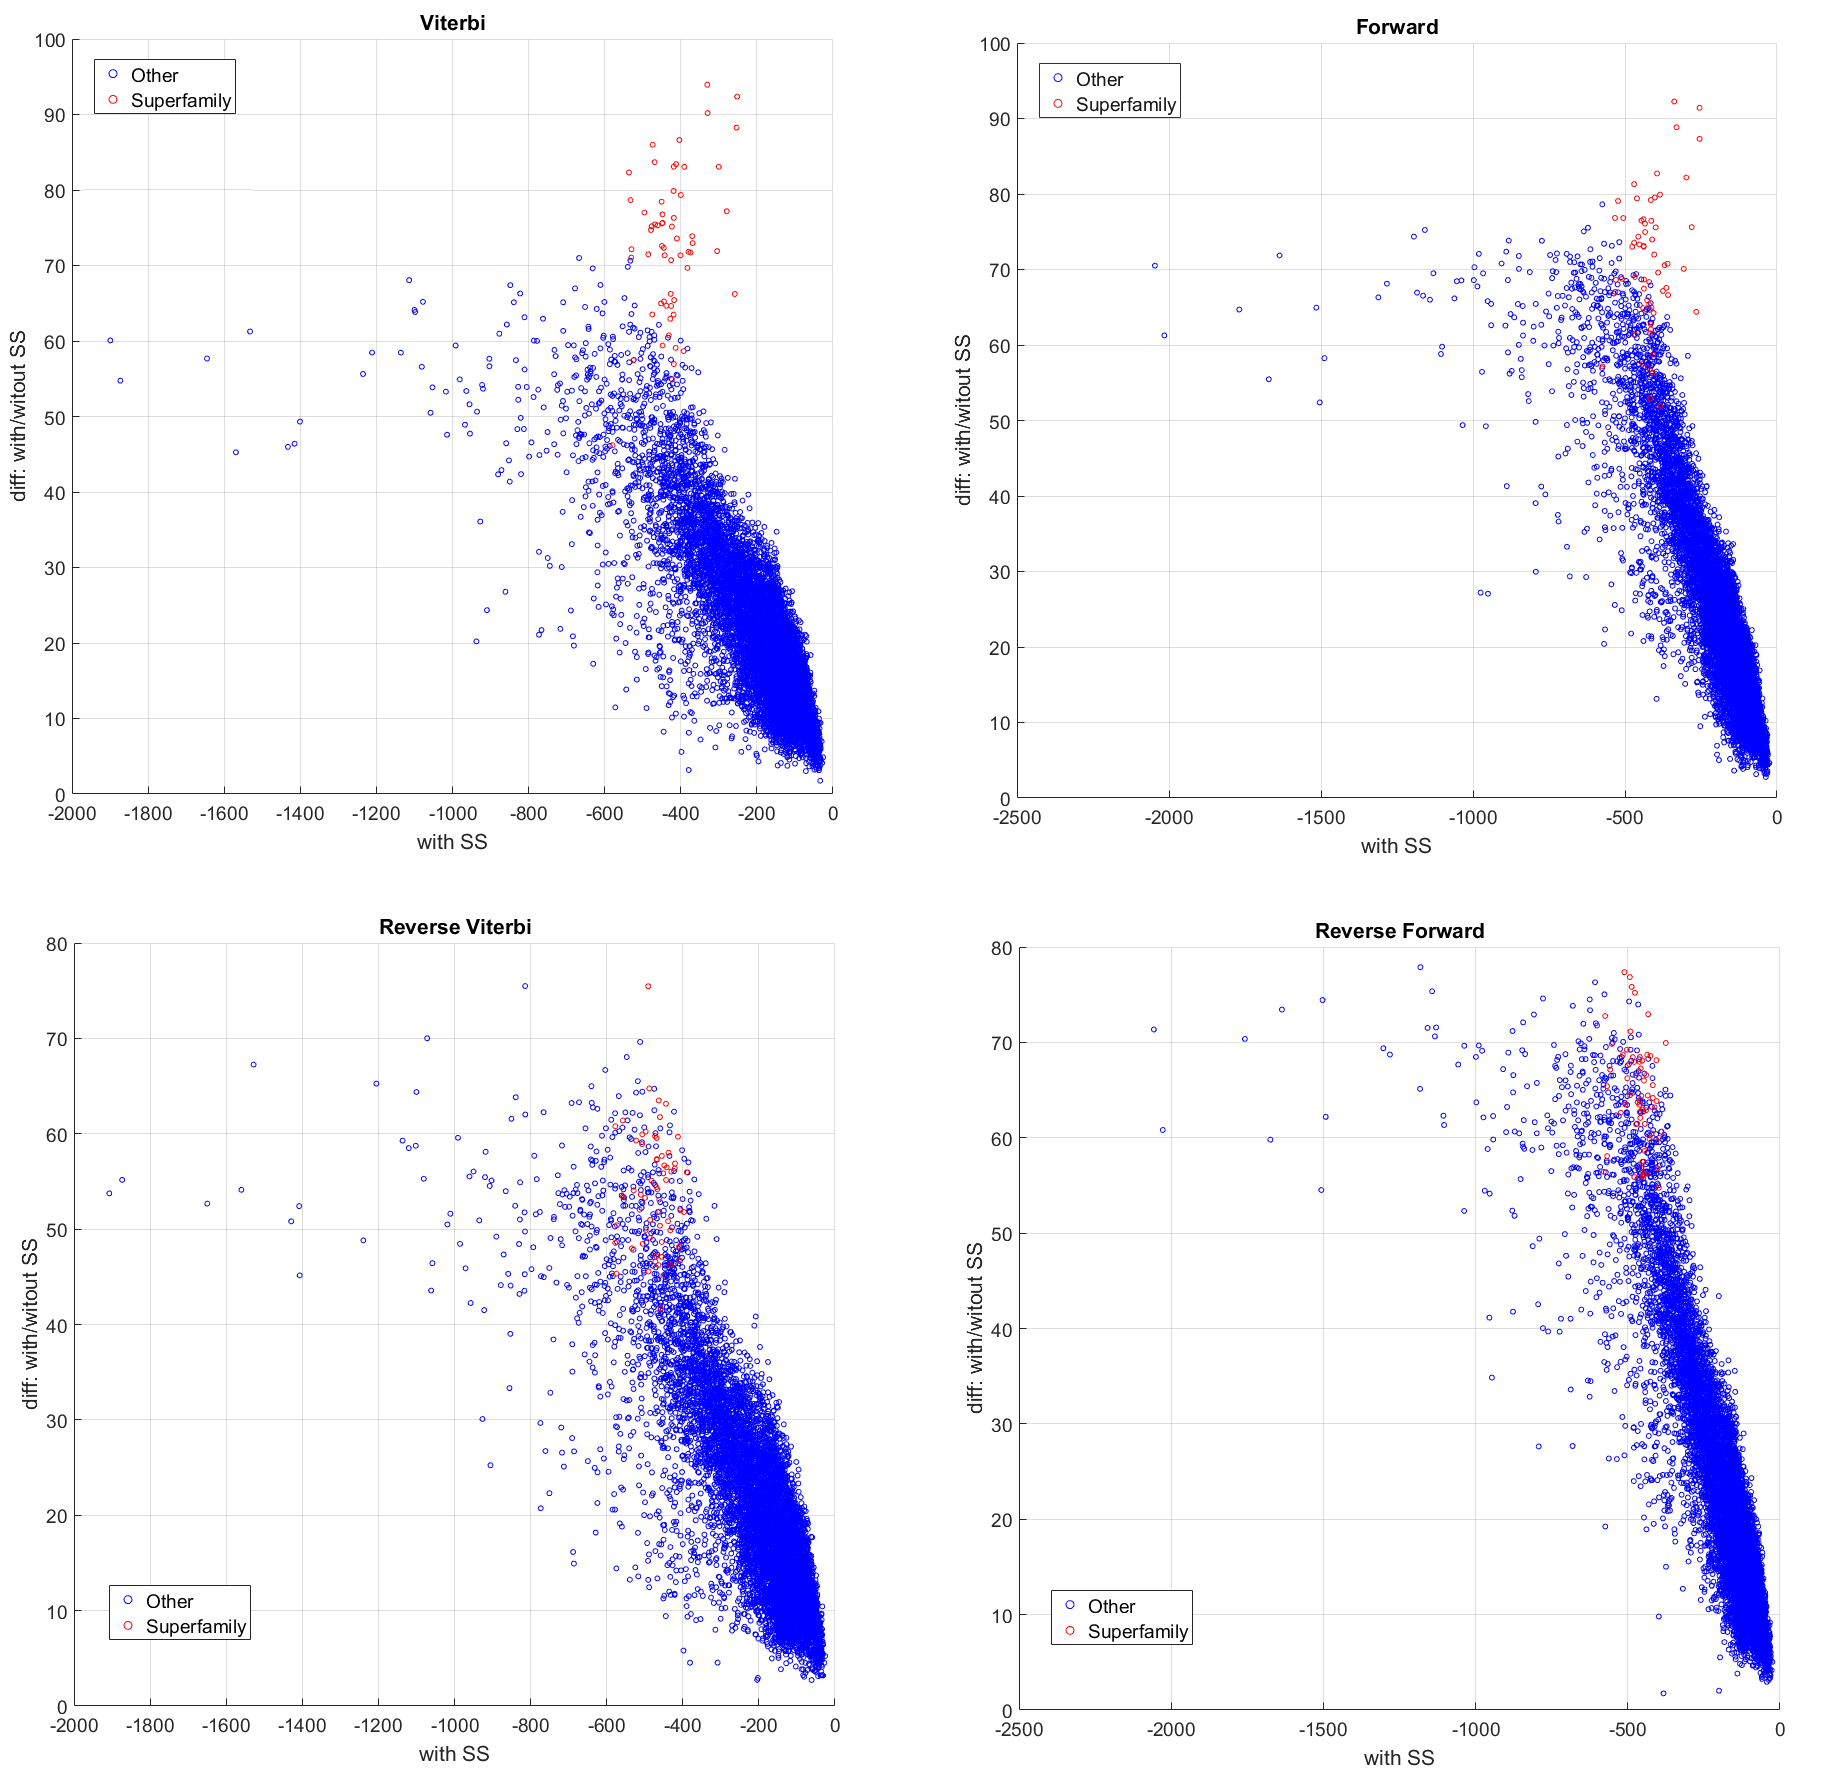
\includegraphics[width=0.97\textwidth]{fig/1plainUreversed}
	\end{center}
	\caption[Comparison between plain scores with and without secondary structure information.]{Comparison between plain scores with and without secondary structure information as scatterplots, with the score including secondary structure on the horizontal axis and on the vertical axis the difference from the scores with and without secondary structure information.}
	\label{fig:eval1}
\end{figure}


 


 
 
 
 %%%%%%%%%%%%%%%%
%%%%%  		Reverse corrected Scores
%%%%%%%%%%%%%%%
Figure \ref{fig:eval1_revCorr} shows the reverse-corrected scores. 
These are the combinations of the plain Viterbi and forward scores with their respective reversed scores in Figure \ref{fig:eval1}, displayed as a scatterplot of the scores with and without secondary structure information. The horizontal axis of the plot shows the original scores obtained using only the primary structure. The vertical axis gives the corresponding scores calculated by including the secondary structure. The red line straight through the origin assists in identifying the change in each score. Scores where the original score equals the new score are positioned on the red line. The farther away a score is from the zero line, the larger the change in the score between the two methods. Scores above the line indicate an increase; scores below the line mark a decrease in the score when including secondary structure information.  
A so-called \textit{rug plot} is included in the following figures. The rug plot is a one-dimensional representation of the data points projected along the axis. These rug plots are separated for scores from the superfamily, indicated as red ticks, and the other points, shown as blue ticks.  

 \begin{figure}[h!]
	\begin{center}
		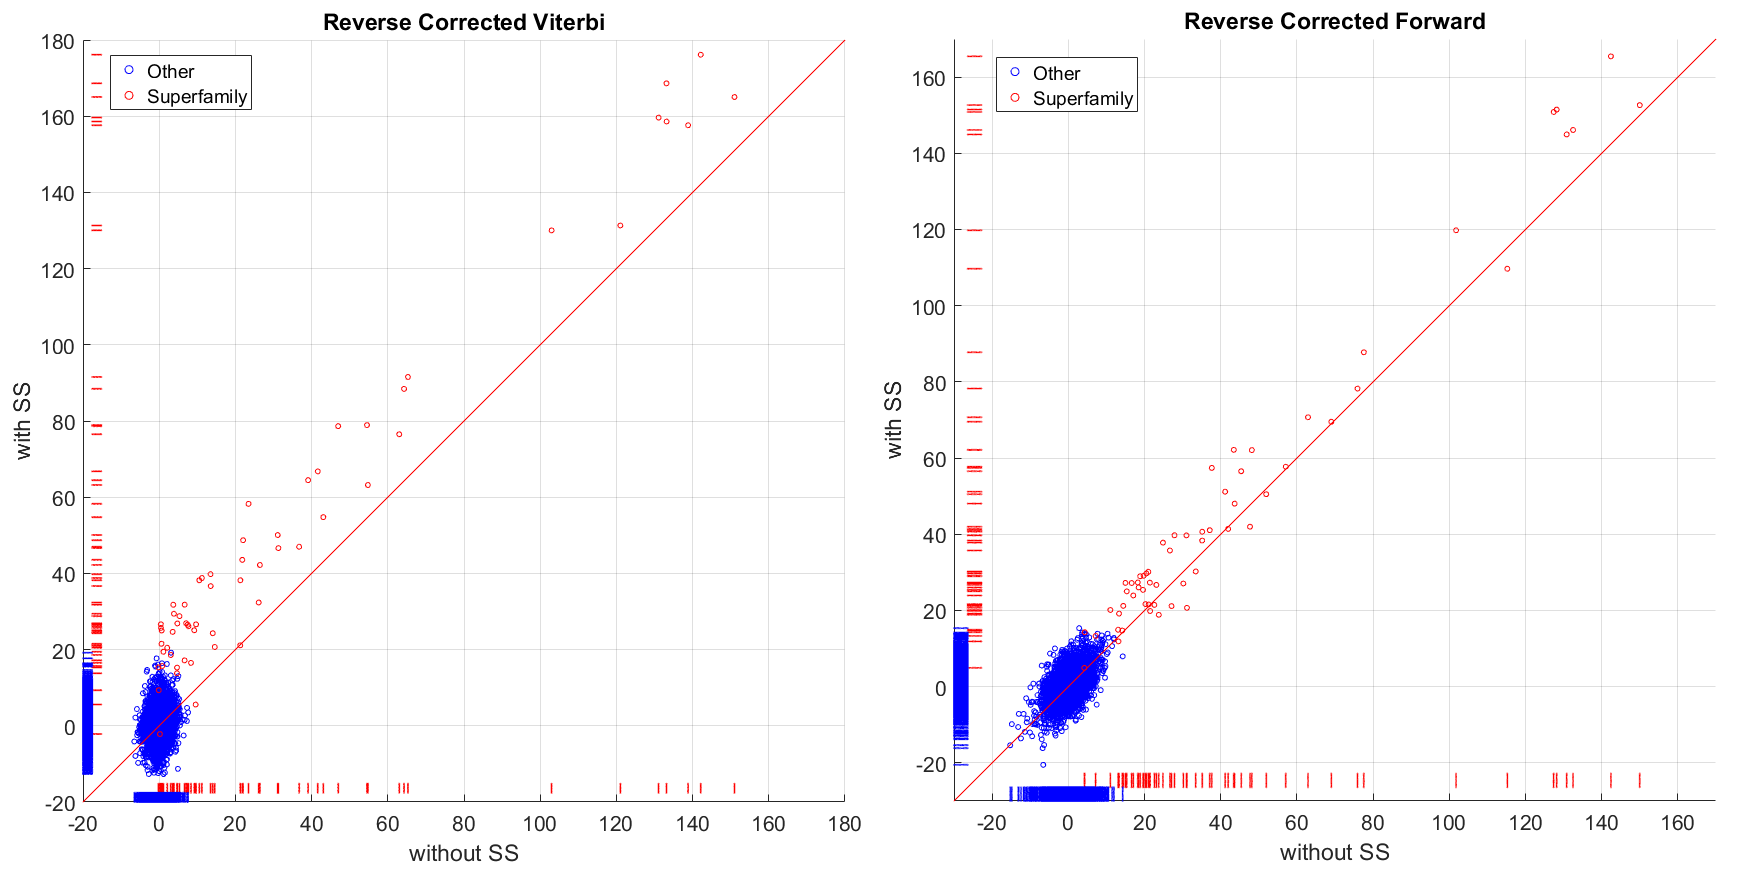
\includegraphics[width=0.99\textwidth]{fig/corr_4}
	\end{center}
	\caption[Scatterplots for comparing reverse-corrected scores with and without secondary structure information.]{Scatterplots for comparing reverse-corrected scores with and without secondary structure information on the horizontal axis and with secondary structure information in the vertical axis. }
	\label{fig:eval1_revCorr}
\end{figure}



Noticeable for the reverse-corrected Viterbi score is the dispersal of the other scores over twice the region when using secondary structure information. This difference is interesting due to its average change of below 0.5. However, except for three scores, the superfamily scores increase consistently. In particular, most superfamily scores close to zero and therefore surrounded by other scores increase more than the average and move away from the other scores. In contrast, the dispersal of the other scores for reverse-corrected forward scores remain closer to region of the original score. In addition, the rise of the superfamily scores is lower. While several low scores perform better than the other scores, there are also some decreasing superfamily scores.





Figure \ref{fig:eval1_simp} shows the same plot as Figure \ref{fig:eval1_revCorr}, but with the two simple-corrected scores. These are the simple null model scores subtracted from the plain Viterbi and forward scores. The simple null model uses the same general background distribution; therefore, there is no change when including secondary structure information. As a consequence, the region of all scores for the two simple-corrected scores increases according to the average score change listed in Table  \ref{tab:LST_Scores}. Moreover, except for a few outliers, the superfamily scores separate clearly from the other scores.


\begin{figure}[H]
	\begin{center}
		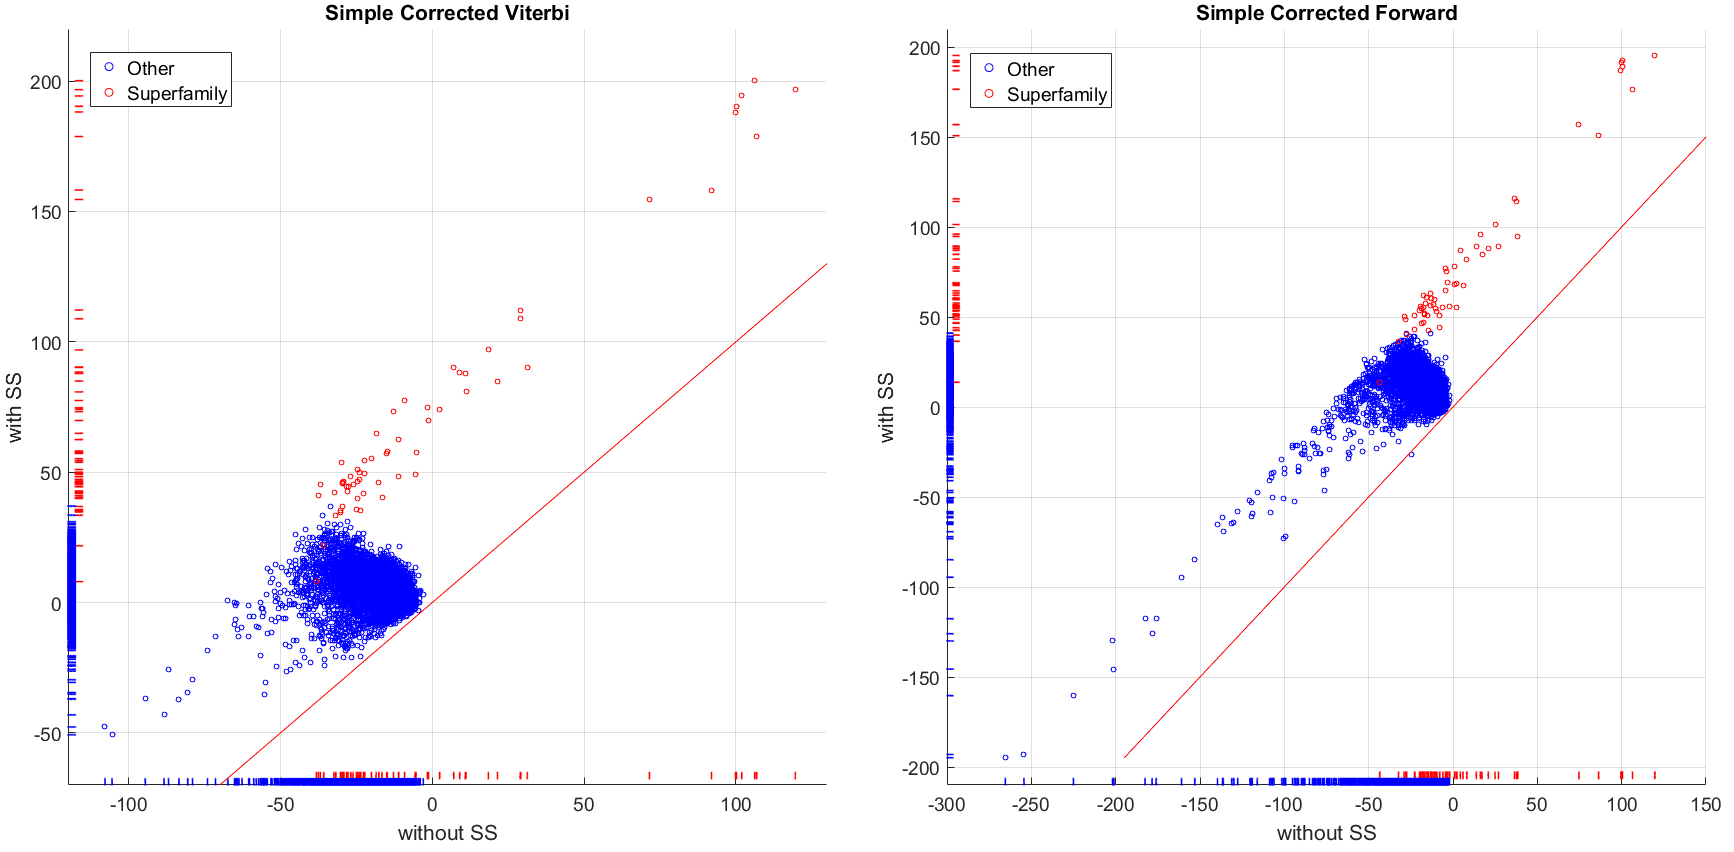
\includegraphics[width=0.92\textwidth]{fig/1simpleCorr}
	\end{center}
	\caption[Scatterplots for comparing simple-corrected scores with and without secondary structure information.]{Scatterplots for comparing simple-corrected scores with only the primary structure information on the horizontal axis with scores calculated using secondary structure information on the vertical axis. }
	\label{fig:eval1_simp}
\end{figure}



\section{Combining Scores}

\begin{table}[b]
	\centering
\begin{tabular}{|llrr|}
\hline
Method & Family & SS score \quad  & \qquad PCA score \\ \hline

Simple corrected Viterbi	& Superfamily: & +72.7664 & \qquad +64.3552 \\ 
    						& Other:       & +21.8893 &  +17.2243 \\ \hline
Simple corrected forward	& Superfamily: & +71.0713 &  +50.0806 \\ 
    						& Other:       & +25.1106 &  +16.0857 \\ \hline


Reverse corrected Viterbi	& Superfamily: \qquad \qquad & +18.8087  &  +27.4886 \\ 
    						& Other:       & +0.56383 &  $-$0.41845 \\ \hline
Reverse corrected forward \qquad	& Superfamily: & +6.34041 & +21.3730 \\ 
    						& Other:       & +0.42186 & $-$0.55353 \\ \hline
\end{tabular}
	\caption{Average change for \acs{MSA} c.67.1 using primary structure only to the \acs{PCA} optimized score.}
	\label{tab:LST_ScoresPCA}
\end{table}




\acp{PCA} is a statistical approach that uses orthogonal transformation in order to reduce the dimensions of correlated data while preserving as much variability and thus information as possible (see \citep{Dunteman.1989}).
In consideration of the difference between the score with secondary structure information and those without, a linear combination of both scores might further improve the results. 
This is done by using \ac{PCA} to obtain the first principle component  of the two-dimensional data containing the score with and without secondary structure information. 


Table \ref{tab:LST_ScoresPCA} lists the average changes between the scores without secondary structure information and the first principal component of the same score, and the score including secondary structure. The column \textit{SS-Score} lists the average change without applying \ac{PCA} (see Table \ref{tab:LST_Scores}). Applying \ac{PCA} on both simple-corrected scores reduces the average change from the scores without secondary structure information by up to 36\,\%. In contrast, the superfamily scores for both reverse-corrected scores increase significantly, while the other scores decrease. 

The impact of using \ac{PCA} is shown in Figure \ref{fig:eval1CorrPCA} with scatterplots of the \ac{PCA}-generated scores over the scores with secondary structure. Both simple-corrected scores suffer from high deterioration. The scores in the transition region perform even more poorly, where the superfamily scores should separate from the other scores. On the other hand, the reverse-corrected scores provide a better result. The superfamily scores increase more than the other scores. Some of the reverse-corrected Viterbi scores decline in the transition area, but in the same region there is also a drop in the other scores.

\begin{figure}[H]
	\begin{center}
		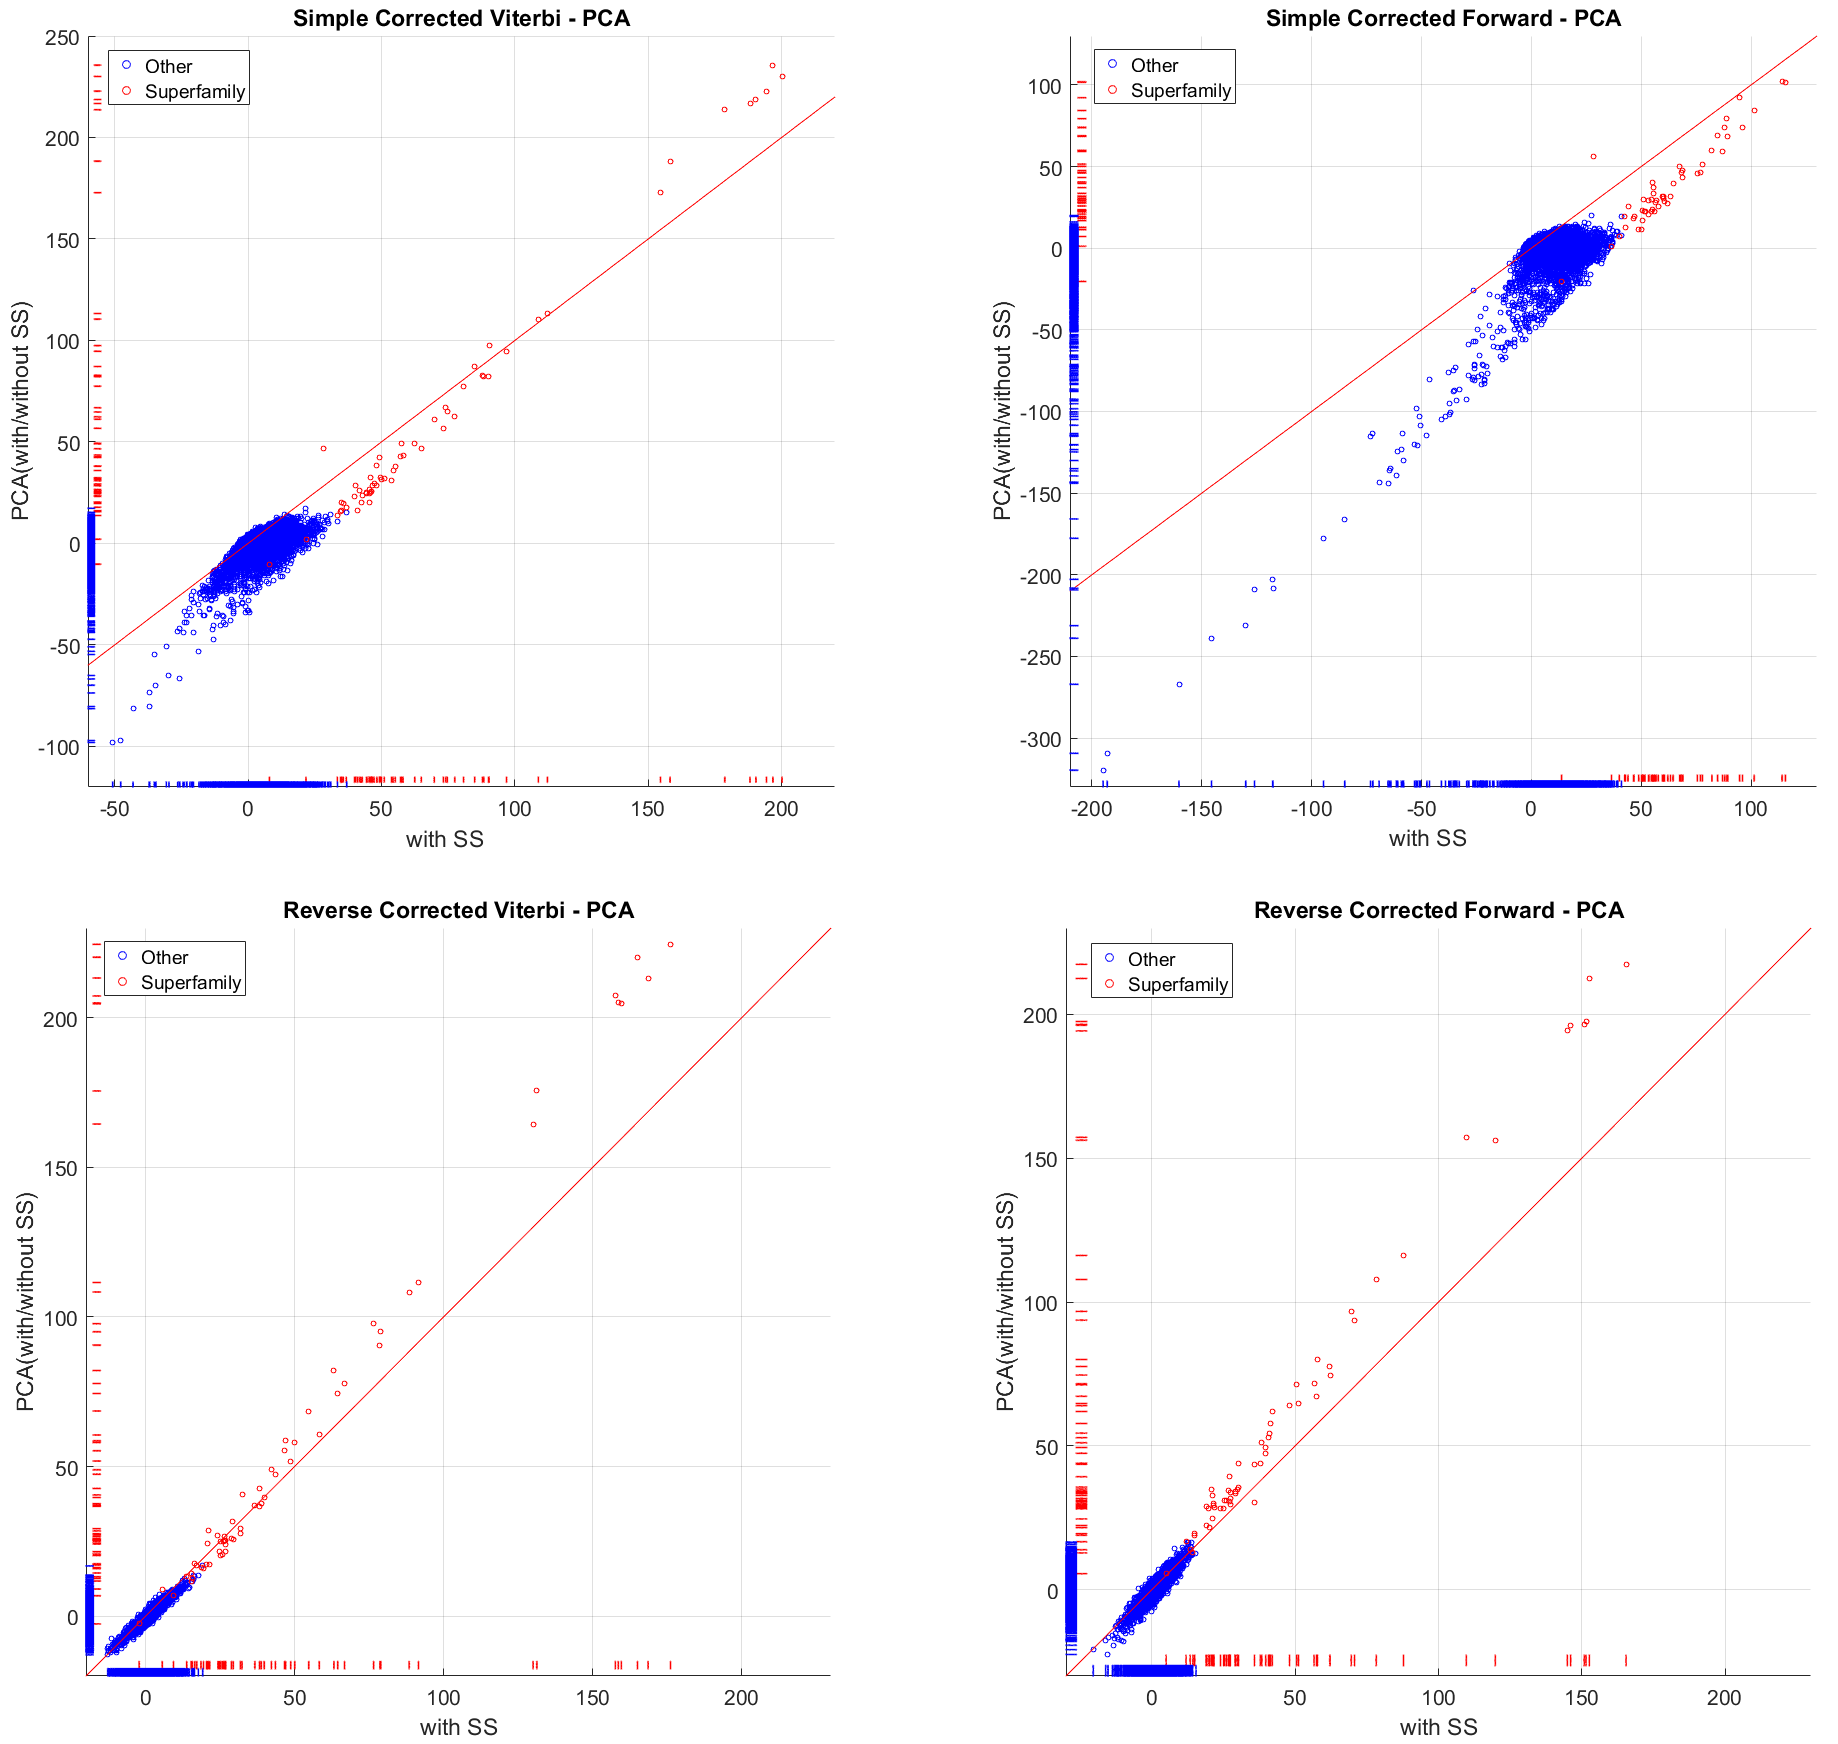
\includegraphics[width=0.9\textwidth]{fig/PCA/corr_pca}
	\end{center}
	\caption[Comparison of scores corrected by applying \acs{PCA}. ]{Comparison of scores corrected by applying \acs{PCA} over the secondary structure scores.}
	\label{fig:eval1CorrPCA}
\end{figure}


From the figures shown previously in this chapter, it is obvious that the scores for both methods, i.e. the Viterbi algorithm and the forward algorithm, are highly correlated. Therefore, a linear combination of the scores from the same type should reduce the dimensional complexity of the data by uniting the information from each method. 

\aclp{PCA} was applied separately on both simple-corrected and reverse-corrected scores. 
These new scores are shown in Figure \ref{fig:PCAcorrSame} on the vertical axis over their associated Viterbi score on the horizontal axis. The mostly linear distribution shows that scores from the same type but different methods mostly share the same information. An exception is the lower section of the scores not related to the \texttt{c.67.1} superfamily. The reason for this drop in scores can be found in the distribution of both scores, visualized in the rug plot in Figure \ref{fig:eval1_simp} on the vertical axis. While both superfamily scores are spread around the same region, the other scores from the forward algorithm are spread over four times the area compared to those from the Viterbi algorithm.  

\begin{figure}[H]
	\begin{center}
		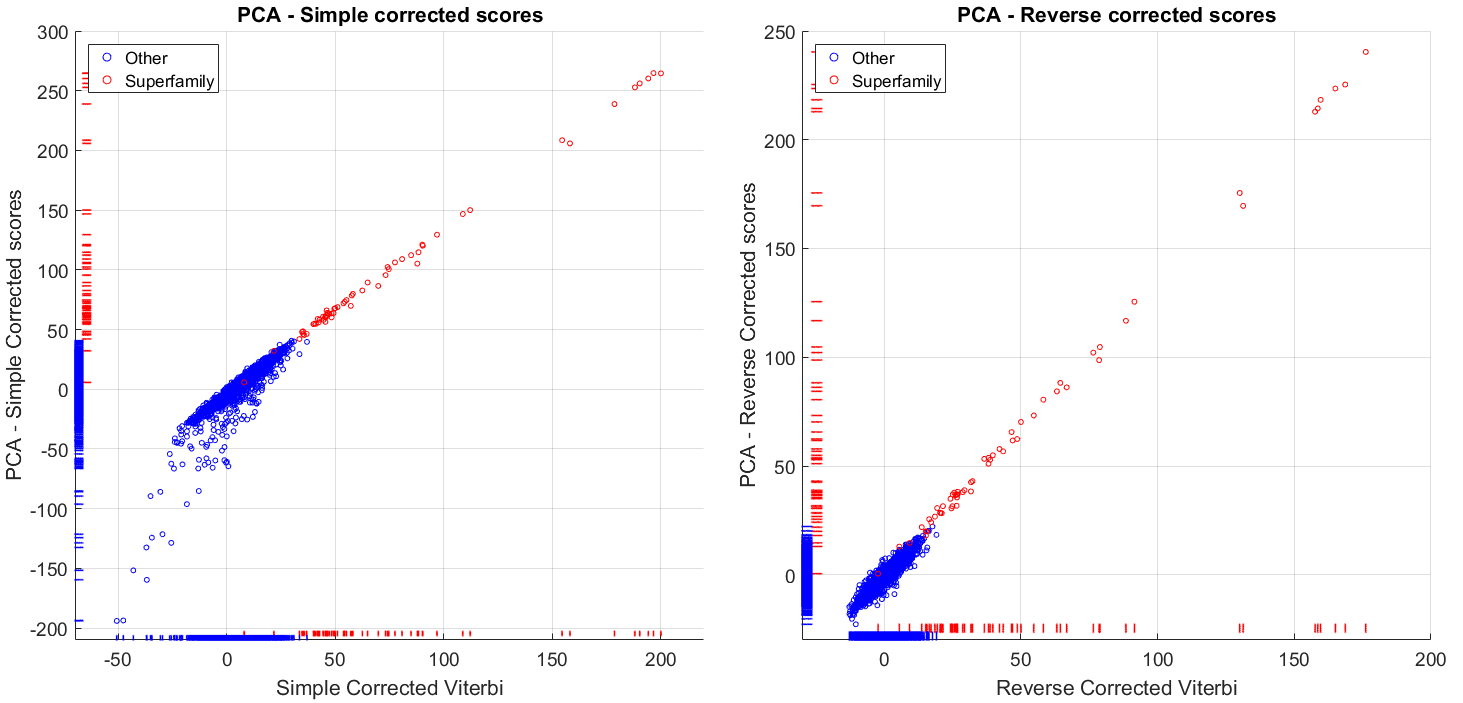
\includegraphics[width=\textwidth]{fig/PCA/pca_both_same}
	\end{center}
	\caption{\acs{PCA} applied to the scores over the Viterbi and forward methods.}
	\label{fig:PCAcorrSame}
\end{figure}

 




Up until this point, the focus was mainly on the single scores, mostly from the same type and method, to improve the separation between the scores of the \ac{MSA} superfamily and the others. The following section analyzes the reverse-corrected scores and the simple-corrected scores from the same method together.
 

Figure \ref{fig:scatter} shows scatterplots with the simple-corrected scores on the horizontal axis and the reverse-corrected scores on the vertical axis, generated from the original score with the primary structure only on top, and including the secondary structure information below. For both approaches, Viterbi and forward scoring, the improvements using the secondary structure are obvious, as the separation between the superfamily scores and the others increases. 
However, this result was already expected based on the figures provided in this section. The same plot for all other variations of the \ac{MSA} \texttt{c.67.1} shown in this section can be found in Appendix \ref{app:APPPCAcorrScores}. 


\begin{figure}[H]
	\begin{center}
		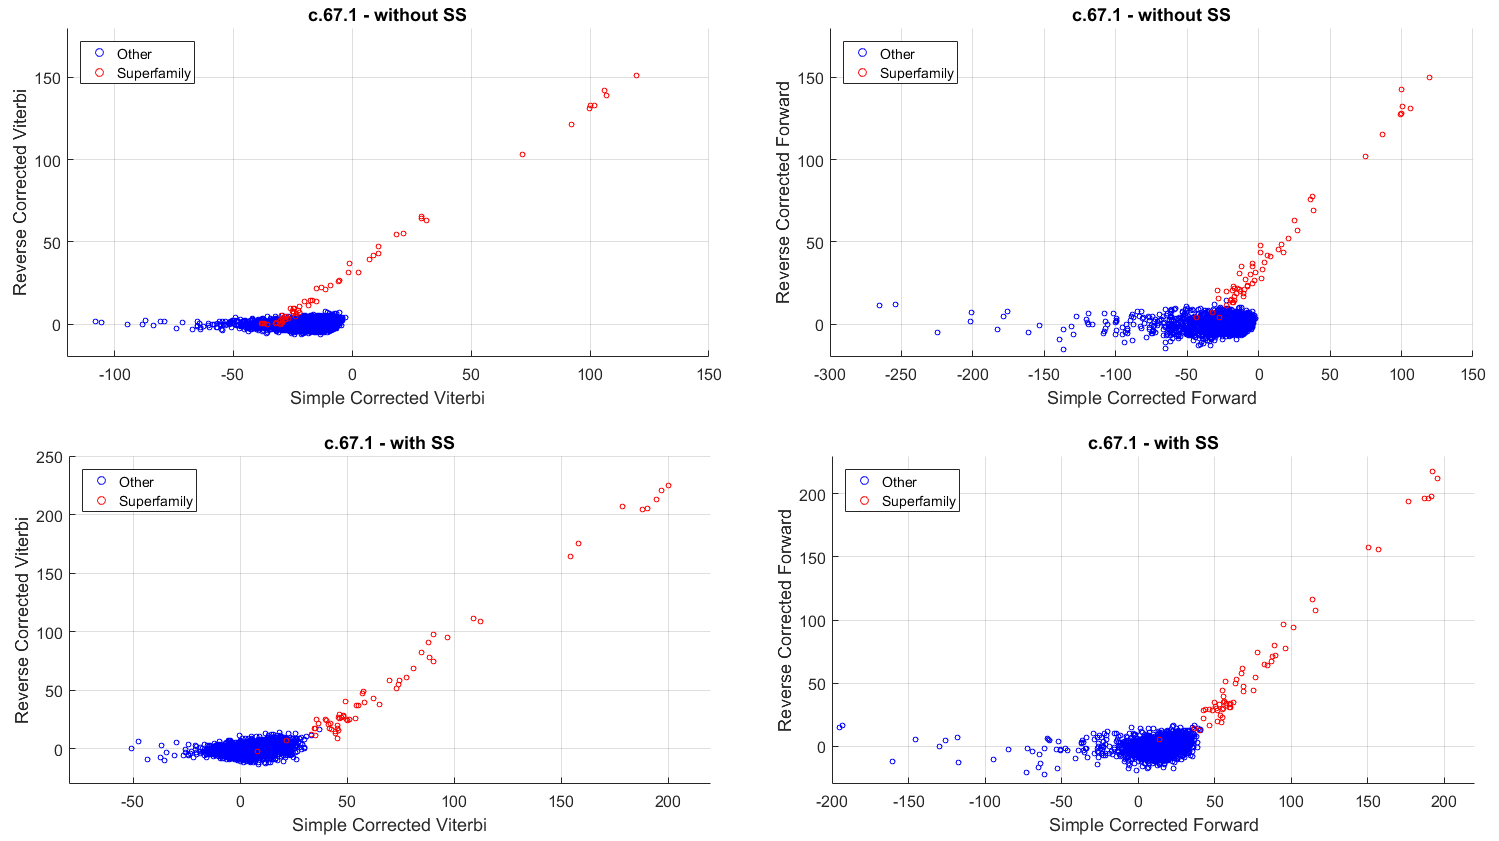
\includegraphics[width=\textwidth]{fig/scatter}
	\end{center}
	\caption{Scatterplots of the corrected scores with and without secondary structure information.}	
	\label{fig:scatter}
\end{figure}

This two-dimensional representation with its variety of post-processing methods is used in the following section for the evaluation of all 69 \acp{MSA} with varying weighting methods.


\section{Evaluation of the Different Weighting Methods}
\label{sec:weightingMeth}

The different weighting methods and their parameters described in  Section \ref{sec:training} will be tested by scoring all 69 \acp{MSA} against the \ac{SCOP} database with different settings. The following five configurations will be explained in more detail.

\begin{itemize}
\item \texttt{M1\_025\_1} uses the weighting approach in (\ref{eq:mix1}), with a pseudo-count of 1 for the secondary structure emission probabilities and a threshold of 0.25 for the highest primary structure emission probability. 

\item \texttt{M1\_025\_3} uses the same approach as above, except with a pseudo-count of 3.

\item \texttt{M2\_025\_1\_3} uses the weighting approach in (\ref{eq:mix2}), also with a threshold of 0.25 and a pseudo-count of 1. The scale factor $k$ is set to 3. 

\item \texttt{M2\_025\_1\_5} uses the same parameters as M2\_025\_1\_3 except with a scaling factor of 5.

\item \texttt{M3\_100\_5} uses the Shannon approach in (\ref{eq:shannonfinal}) with a pseudo-count of 5 for generating the secondary structure emission probabilities. A threshold of 100\,\% is also employed, resulting in only the mixed probabilities being used for scoring.
\end{itemize}

For example, with the \ac{MSA} \texttt{c.67.1}, the threshold of 0.25 for the first four approaches results in 272 columns where the highest emission probability is below the threshold; therefore, the mixed probabilities are used, containing both the primary and the secondary structure. For the other 117 columns of the \ac{pHMM}, only the emission probabilities for the primary structure are used. For the last method, using the Shannon entropy, it was found that the best results are achieved using the mixed probabilities only.

The different methods over the \acp{MSA} are compared in MATLAB as listed in \ref{LST_svmMat} by generating a \ac{ROC} curve. A \ac{ROC} curve compares the \ac{TPR} against the \ac{FPR} for varying thresholds of a classifier and is used to compare the quality of classifiers. The \ac{TPR} measures the proportion of positives that are correctly classified as such, while the \ac{FPR} identifies negatives that are wrongly classified as positives (see \cite[p. 34--35]{Duda.2001}).

\lstset{
keywords={fitcsvm, fitPosterior, resubPredict, perfcurve},numbers=left, captionpos=b,	tabsize=4, numbersep=10pt, commentstyle=\color{dkgreen}, keywordstyle=\color{blue},
	showspaces=false, 
basicstyle  = \fontfamily{pcr} \fontsize{9pt}{10pt} \selectfont \singlespacing ,}
\begin{lstlisting}[caption=Matlab implementation for generating the \ac{ROC} curve. ,
label=LST_svmMat]
mdlSVM = fitcsvm(hmmScores,classes,'Standardize',true);
mdlSVM = fitPosterior(mdlSVM);
[~,score_svm] = resubPredict(mdlSVM);
[X,Y,T,AUC] = perfcurve(hmmScores,score_svm(:,mdlSVM.ClassNames),'true');
plot(X,Y)
\end{lstlisting}

 For each method and \ac{MSA}, the function \textit{fitcsvm} trains a binary \ac{SVM} classifier from \textit{hmmScores}, containing the two dimensions for the reverse-corrected and the simple-corrected scores and the \textit{classes}, indicating whether the score relates to the tested superfamily or not. The function \textit{fitPosterior} calculates the posterior probabilities for all scores, allowing \textit{perfcurve} to generate the \ac{ROC} curve.



Figure \ref{fig:roc} shows the \ac{ROC} curve generated for the superfamily \texttt{c.67.1} using the methods described above, as well as the original score using only the primary structure listed as \textit{AA}. The scores used are the two corrected Viterbi scores, with the \mbox{reverse-corrected} Viterbi as the first principal component from the score with and without secondary structure information.
The six scatterplots used for this \ac{ROC} plot are shown in Appendix \ref{app:APPPCAcorrScoresWeight}.
As an optimal classifier would be a rectangular graph with 100\% \ac{TPR}  at 0\% \ac{FPR}, the improvement of the new methods using secondary structure information is obvious.

\begin{figure}[H]
	\begin{center}
		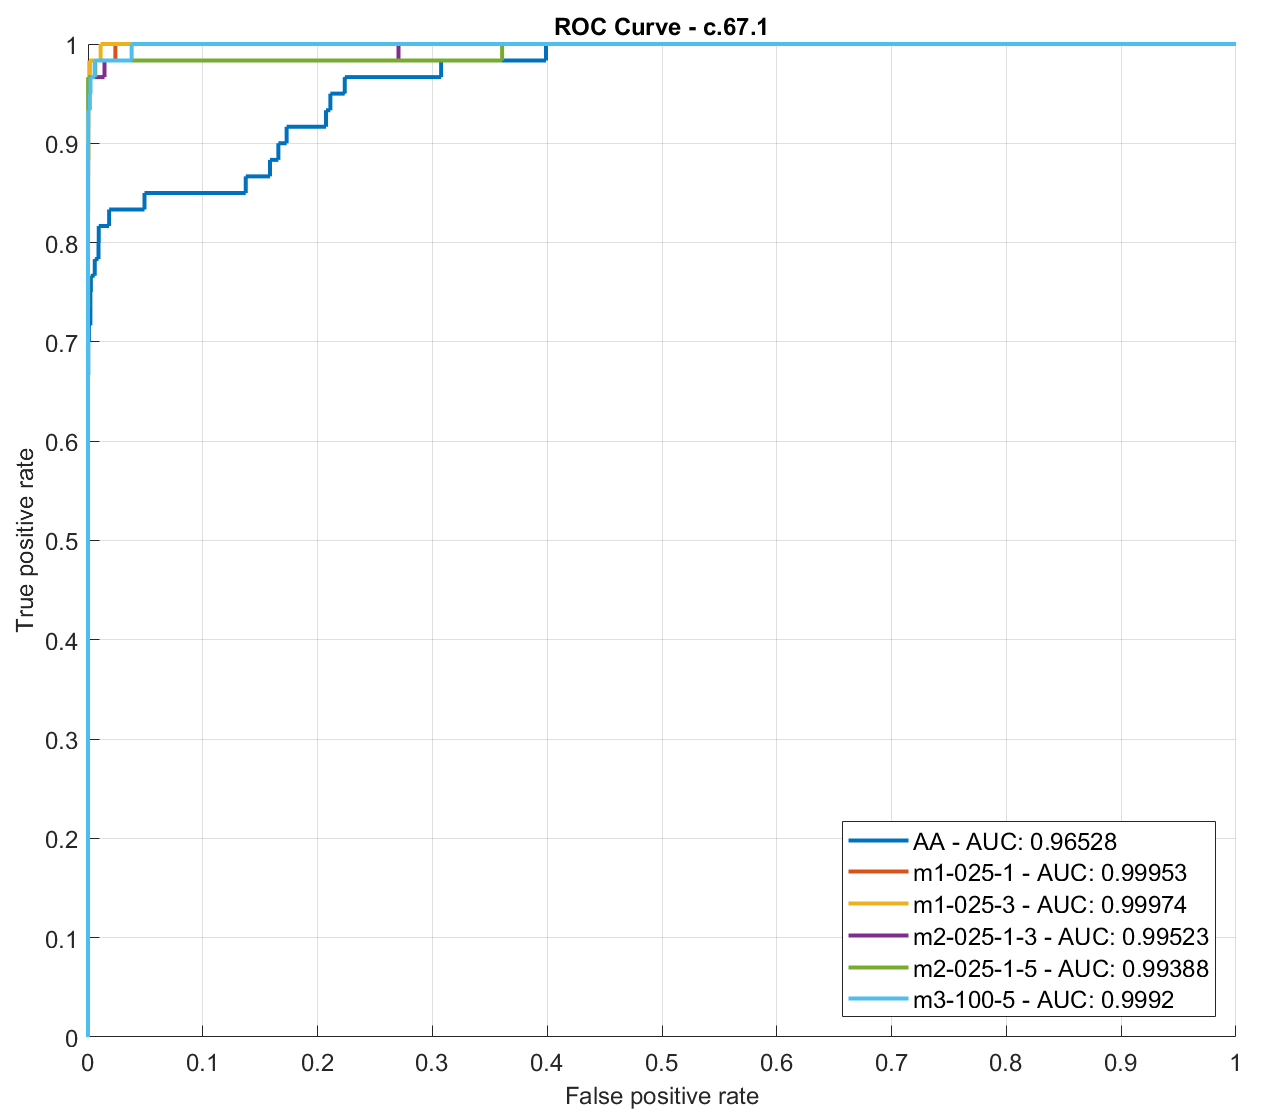
\includegraphics[width=0.8\textwidth]{fig/roc}
	\end{center}
	\caption{\acs{ROC} curve for the \acs{MSA} c.67.1.}
	\label{fig:roc}
\end{figure}

For comparison of the different methods, the \ac{ROC} curves can be ranked with the \ac{AUC} score. The \ac{AUC} score combines the whole \ac{ROC} curve into one number in the range of 0--1 and is calculated by the integral of the curve. 

Table \ref{tab:ROC} provides an overview of the selected methods for the \ac{MSA}. However, the table lists only 56 \acp{MSA}, as those with  a variation of the AUC score below 1\% were filtered out. Column \textit{AA} lists the \ac{AUC} score using only the primary structure. The highest \ac{AUC} score for each \ac{MSA} is highlighted in green, while all scores below those obtained using the original method  are highlighted in red. To summarize the table, it can be said that except for a few scores, the secondary structure information improves the quality of the homology detection. For all \acp{MSA}, the original score was improved by at least one method including the secondary structure. The best results were achieved with the method \texttt{M2\_025\_1\_5}, with only two scores below the original score and 29 with the highest rank. 


The \ac{AUC} scores for all \acp{MSA} were also compared to the different corrected scores and their combinations discussed in Section \ref{ssec:Scores_Changes}. 
The results are summarized in Table \ref{tab:ovAllAUC}, with the first number of each cell providing the number of scores above those of the original method using only the primary structure. The second number counts the \acs{MSA} with the highest \ac{AUC} scores compared to all other methods. The table shows that the method \texttt{M2\_025\_1\_5} performed best for the most score types, compared to the other methods. The best score type varies across the different methods. For the highest-ranked method, the Viterbi method performs better than the old method for 65 of 69 scores.  However, over all methods, both \ac{PCA} variations for the Viterbi yield a larger improvement than the plain scores. The last column represents the combination of the Viterbi and forward scores. 
In general, this score type performs worse than the other types, with seven \acp{MSA} where the original method has higher scores than all methods that use the secondary structure information.


\definecolor{Gray}{gray}{0.9}
\newcolumntype{g}{>{\columncolor{Gray}}r}
\newcolumntype{h}{>{\columncolor{Gray}}l}
\begin{table}[h!]
\centering
\begin{tabular}{|l|g:h|r:l|g:h|r:l|g:h|}
         \hline
 \multirow{2}{*}{\backslashbox{\small{Method}}{\small{Score-type}}}      & \multicolumn{10}{c|}{ \# scores with AUC > AA ; \# highest scores for method } \\
              & \multicolumn{2}{c|}{Viterbi}                       & \multicolumn{2}{c|}{Forward} & \multicolumn{2}{c|}{PCA-Vit.} & \multicolumn{2}{c|}{PCA-For.} & \multicolumn{2}{c|}{PCA-VitFor} \\ \hline
AA     		  & 					  			&  \: 1 			   & 			 & \: 1      			&               & \: 2          &               &  \: 2    			       	&                  & \: 7  \\ \hline
M1\_025\_1    & 55                    			& 13                   & 54          & 12         			& 60            & \: 8          & 62            & 12     			        & 55              & 11             \\ \hline
M1\_025\_3    & 57                    			& 16                   & 56          & 16         			& 59            & 16            & 63            & 11       					& 51              & 13             \\ \hline
M2\_025\_1\_3 & 49                    			& \: 4                 & 50          & \: 4         		& 54            & \: 4          & 58            & \: 2    			        & 53              & \: 5              \\ \hline
M2\_025\_1\_5 & 65                    			& 28                   & 64          & 28         			& 64            & 33            & 62            & 29       					& 56              & 27             \\ \hline
M3\_100\_5    & \quad 55             			& \: 7            & \quad 46         & \: 8          		& \quad 54      & \: 6            & \quad 59      & 13             & \: \: 55              & \: 6        \\  \hline
\end{tabular}
	\caption[Performance of different scoring methods.]{Performance of different scoring methods for the corrected scores over all 69 \acsp{MSA}. First column lists number of \acs{AUC} scores above the score using primary structure only (AA), second column number of highest scores for the method. }
	\label{tab:ovAllAUC}

\end{table}

The \ac{AUC} scores for each score type and the method of all 69 \acp{MSA} represented in Table \ref{tab:ovAllAUC}, including their associated scatterplots and ROC curves, can be found on the attached disk (see Appendix \ref{app:AppDisk}).




\def\g{\cellcolor{green!25}}
\def\r{\cellcolor{red!25}}
\def\y{\cellcolor{yellow!10}}

% Please add the following required packages to your document preamble:
% \usepackage{graphicx}
\begin{table}[H]
\centering
\resizebox{\textwidth *6/7}{!}{%
 \renewcommand{\arraystretch}{0.8}
\begin{tabular}{|l|c|ccccc|}
\hline
MSA      &  AA  \qquad & M1\_025\_1 & M1\_025\_3 & M2\_025\_1\_3 & M2\_025\_1\_5 & M3\_100\_5 \\ \hline
a.1.1   & \enskip \y 0.981660 \enskip & \enskip \g 0.999138 \enskip   &  \enskip 0.998953 \enskip  & \enskip 0.992644 \enskip     & \enskip 0.997789 \enskip     &  \enskip 0.997729 \enskip   \\ 
a.118.1 & \y 0.658467      & 0.753259      & 0.705426      & 0.746597      & \g 0.829309      & \r 0.644325       \\
a.118.8 & \y 0.955319      & 0.984794      & 0.985946      & \g 0.986001      & 0.973027      & 0.977922       \\
a.121.1 & \y 0.949624      & 0.995763      & 0.995620      & 0.996995      & \g 0.997438      & 0.983587       \\
a.25.1  & \y 0.841495      & 0.937005      & 0.932636      & 0.941242      & \g 0.957592      & 0.937555       \\ \hline
a.26.1  & \y 0.874773      & 0.983614      & 0.985165      & 0.969996      & \g 0.985939      & 0.964079       \\
a.39.1  & \y 0.952474      & 0.981174      &  \g 0.982275      & 0.959055      & 0.979119      & \r 0.948074       \\
a.4.1   & \y 0.943772      & 0.955631      & 0.952669      & \g 0.969677      & 0.964489      & \r 0.918509       \\
a.4.5   & \y 0.855347      & 0.926701      & 0.925346      & 0.908423      & \g 0.929703      & 0.916538       \\
b.1.18  & \y 0.792153      & 0.817158      & 0.807228      & 0.815886      & \g 0.838580      & 0.802668       \\  \hline
b.1.2   & \y 0.969961      & 0.995894      & 0.995995      & 0.981565      & 0.993793      & \g 0.997065       \\
b.121.4 & \y 0.773631      & 0.967558      & 0.966382      & 0.866694      & \g 0.992417      & 0.953065       \\
b.122.1 & \y 0.848138      &  \r 0.845888      &  \r 0.848104      & \r 0.845576      & \g 0.851568      &  \r 0.779088       \\
b.18.1  & \y 0.761240      & 0.930075      &  \g 0.936217      & 0.817446      & 0.866923      & 0.929797       \\
b.29.1  & \y 0.696135      & 0.960836      & 0.951235      & 0.849526      & \g 0.983435      & 0.940170       \\  \hline
b.40.4  & \y 0.562231      & 0.645208      &  \g 0.670961      & 0.569530      & \r 0.338704      & 0.567449       \\
b.55.1  & \y 0.911226      & 0.979285      &  \g 0.980650      & 0.929043      & 0.959400      & 0.957248       \\
b.6.1   & \y 0.908563      & 0.960190      &  \g 0.966697      & 0.937017      & 0.955984      & 0.957871       \\
b.60.1  & \y 0.930032      & 0.984104      & 0.984354      & 0.970134      & \g 0.990348      & 0.978497       \\
b.82.1  & \y 0.825039      & 0.938847      & 0.919836      & 0.866187      & \g 0.955784      & 0.912106       \\  \hline
c.1.10  & \y 0.873501      & 0.874392      &  \r 0.869691      & \r 0.872736      & \g 0.940628      & \r 0.872383       \\
c.1.8   & \y 0.771208      & 0.928533      & 0.936710      & 0.773840      & 0.930788      & \g 0.945124       \\
c.1.9   & \y 0.776061      & 0.984452      &  \g 0.987866      & 0.849393      & 0.953804      & 0.968378       \\
c.14.1  & \y 0.922587      & 0.973523      &  \g 0.978553      & \r 0.895175      & 0.937373      & 0.943083       \\
c.2.1   & \y 0.832922      & 0.877780      &  \g 0.878903      & \r 0.830230      & 0.874660      & 0.849042       \\  \hline
c.23.16 & \y 0.953418      & 0.984812      &  \g 0.985526      & \r 0.946543      & 0.970777      & 0.979098       \\
c.23.1  & \y 0.982697      & 0.997496      & 0.996486      & 0.996668      & \g 0.998236      & 0.994347       \\
c.26.1  & \y 0.948562      & 0.976231      &  \g 0.976961      & 0.960769      & 0.965366      & 0.976797       \\
c.26.2  & \y 0.762557      & 0.851986      & 0.846154      & 0.772628      & \g 0.903711      & 0.878560       \\
c.3.1   & \y 0.873175      & 0.889874      & 0.884938      & 0.874126      & \g 0.900207      & \r 0.855220       \\  \hline
c.37.1  & \y 0.566633      & 0.757238      & 0.705066      & 0.633610      & \g 0.795116      & 0.721068       \\
c.47.1  & \y 0.758197      & 0.851974      & 0.840546      & 0.832753      & \g 0.889316      & 0.819158       \\
c.52.1  & \y 0.715274      &  \r 0.687236      &  \r 0.689456      & 0.728182      & \g 0.729141      & \r 0.689634       \\
c.55.1  & \y 0.841824      & 0.890524      & 0.888006      & 0.872482      & 0.879920      & \g 0.896231       \\
c.55.3  & \y 0.661511      & 0.724718      & 0.730029      & 0.745105      & \g 0.827794      & 0.708841       \\  \hline
c.56.5  & \y 0.932965      & 0.975813      & 0.976139      & \r 0.931557      & \g 0.988531      & 0.970057       \\
c.66.1  & \y 0.691936      & 0.792645      & 0.805687      & 0.762319      & \g 0.828899      & 0.826029       \\
c.67.1  & \y 0.965279      & 0.999527      &  \g 0.999741      & 0.995230      & 0.993875      & 0.999198       \\
c.68.1  & \y 0.840345      & 0.954689      &  \g 0.955924      & 0.896832      & 0.953844      & 0.942945       \\
c.69.1  & \y 0.769510      & 0.951119      &  \g 0.954956      & 0.886774      & 0.945654      & 0.938550       \\  \hline
c.94.1  & \y 0.786186      & 0.885272      & 0.891178      & 0.822143      & \g 0.910847      & 0.838724       \\
d.108.1 & \y 0.842174      &  \g 0.985350      & 0.985037      & 0.890825      & 0.959523      & 0.956787       \\
d.129.3 & \y 0.770835      & 0.906587      & 0.886342      & 0.779503      & 0.887589      & \g 0.929245       \\
d.14.1  & \y 0.800006      & 0.820208      & 0.828362      & 0.813035      & \g 0.884108      & 0.847360       \\
d.144.1 & \y 0.970321      & 0.980958      &  \r 0.968978      & \r 0.968810      & \g 0.985398      & 0.979926       \\  \hline
d.15.1  & \y 0.820850      & 0.841835      & 0.836335      & 0.938895      & \g 0.945733      & \r 0.819833       \\
d.153.1 & \y 0.904484      & 0.963783      &  \g 0.964523      & 0.911143      & 0.941617      & 0.949000       \\
d.169.1 & \y 0.914845      & 0.984051      & 0.986197      & 0.949123      & \g 0.987850      & 0.936318       \\
d.17.4  & \y 0.917448      &  \g 0.997716      & 0.997654      & 0.949466      & 0.988231      & 0.996560       \\
d.3.1   & \y 0.781971      &  \g 0.922795      & 0.913319      & 0.795755      & 0.889231      & 0.920976       \\  \hline
d.32.1  & \y 0.943212      & 0.988796      &  \g 0.991518      & 0.974388      & 0.983423      & 0.983284       \\
d.38.1  & \y 0.927538      & 0.975661      & 0.971830      & 0.955195      & \g 0.986411      & 0.971640       \\
d.58.4  & \y 0.923971      & 0.939588      & 0.928788      & 0.936421      & \g 0.951176      & 0.935353       \\
d.81.1  & \y 0.803026      & 0.821645      & 0.809742      & \r 0.798986      & 0.823577      & \g 0.824889       \\
d.92.1  & \y 0.747920      & 0.791525      & 0.794027      & 0.803735      & \g 0.833569      & 0.819230       \\  \hline
g.39.1  & \y 0.984596      & \r 0.982231      & \r 0.982742      & \g 0.988259      & \r 0.983898      & \r 0.976715  \\ \hline
\end{tabular}%
}
\caption[\acs{AUC} scores for the different scoring methods.]{\acs{AUC} scores for the different scoring methods from the corrected Viterbi scores postprocessed with \acs{PCA} compared to the original method in column AA using primary structure only. The highest score for each \acs{MSA} is marked green. Red scores are below the original method.   }
\label{tab:ROC}
\end{table}





\newpage

\section{Scoring with Predicted Secondary Structure}

The previous tests were all done with secondary structure information gathered via \ac{DSSP} from the three-dimensional structure information. 
Homology prediction is a procedure commonly used for protein sequences for which the three-dimensional structure is unknown.
Furthermore, gaining knowledge about the homology is used to improve methods for determining the proteins tertiary structure.

\begin{figure}[!b]
	\begin{center}
		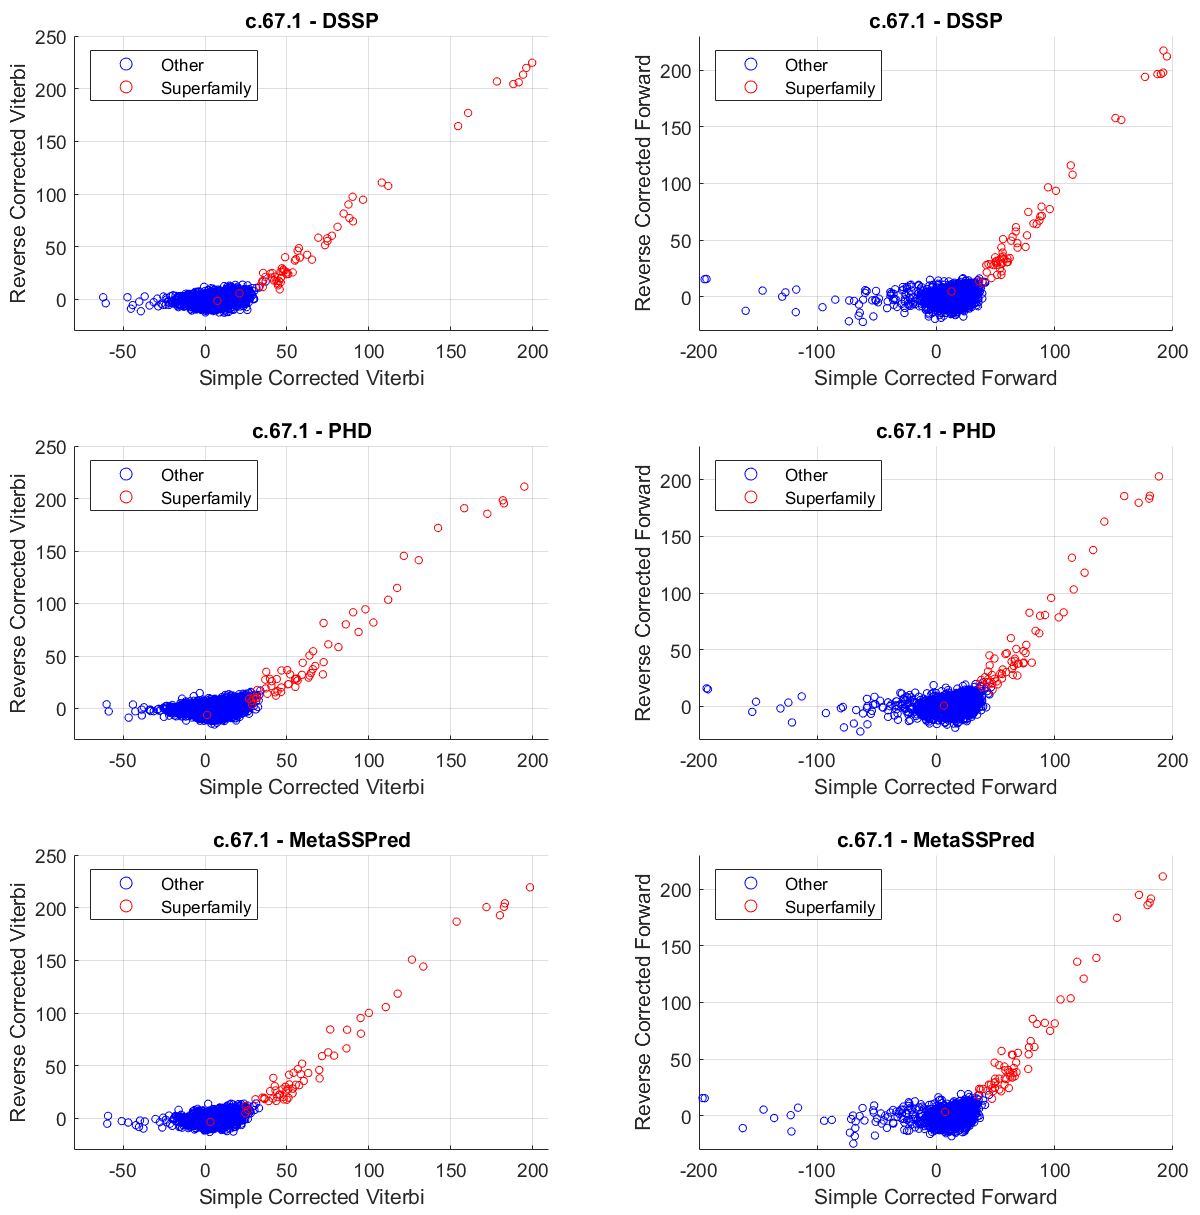
\includegraphics[width=0.97\textwidth]{fig/SS_NE}
	\end{center}
	\caption[Comparision of the different secondary structure estimation methods.]{Comparison of the different secondary structure estimation methods on \acs{MSA} c.67.1. }
	\label{fig:scattBssp}
\end{figure}

The following scatterplots in Figure \ref{fig:scattBssp} compare the results from the different methods of  secondary structure determination on the \ac{MSA} \texttt{c.67.1}. All plots show the simple-corrected scores on the horizontal axis and the reverse-corrected scores on the vertical axis.
 The first row is the reference plot with the secondary structure obtained from \ac{DSSP}.
 The structures for the second and third rows are predicted with \ac{PHD} and MetaSSPred, respectively.  
As in the previous sections, the method \texttt{M2\_025\_1\_3} is used for training the \ac{pHMM} and the test database is scored against it. 
For the \mbox{reverse-corrected} scores, the \ac{PCA} between the scores with and without secondary structure is used. Both the Viterbi scores on the left and the forward scores on the right show a slight decline. Even though the scores in the transition region between the superfamily and the other classes move closer to one another, there is still an outstanding improvement over the scores without secondary structure. This is also apparent in the \ac{ROC} curve in Figure \ref{fig:rocSS} based on the forward scores from Figure \ref{fig:scattBssp} and their associated primary-structure-only scores.

\begin{figure}[H]
	\begin{center}
		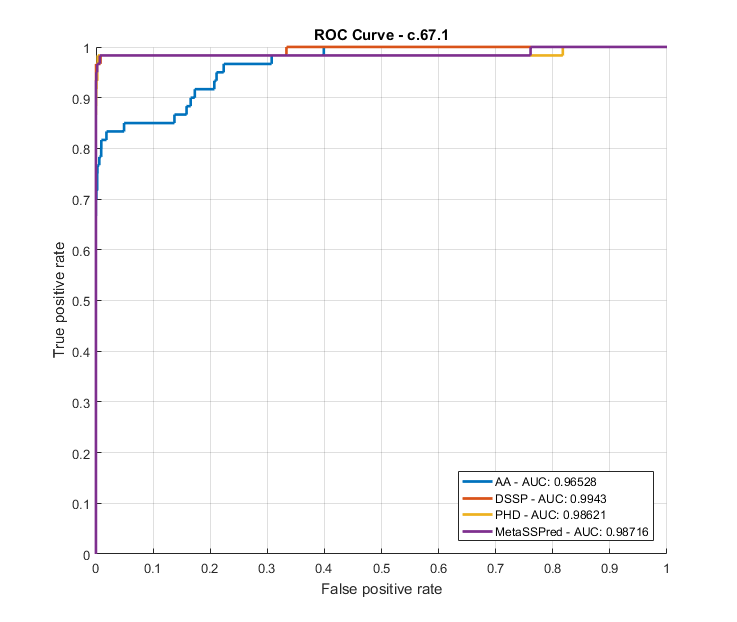
\includegraphics[width=0.8\textwidth]{fig/SSAuc}
	\end{center}
	\caption{\acs{ROC} curves comparing different secondary structure determination methods.} 
	\label{fig:rocSS}
\end{figure}

\chapter{Conclusion}
\label{ch:conclusion}

The following chapter presents a brief summary of the thesis' findings and subsequently provides an outlook of potential future work based on these results.

\section{Summary}

This thesis has presented methods for protein homology detection with \ac{pHMM} using secondary structure information. The key tasks were to determine secondary structure information from primary or tertiary structure, build a \ac{pHMM} using both primary and secondary structure information, and extend the scoring methods to make use of secondary structure information. These steps were implemented in the software package HMModeler. 

Chapter \ref{ch:selectedBG} introduced the biological background of proteins. The discussion included the fundamentals of proteins, their composition by chains of amino acid residues, and their structural levels. Furthermore, relevant databases containing different levels of protein information were introduced. Finally, the statistical model \ac{pHMM} for analyzing proteins was presented.



Chapter \ref{ch:PSD} focused on methods for determining the different structural levels of proteins. This covered protein sequencing and experimental methods for determining the three-dimensional structure on an atomic level. Subsequently, the secondary structure annotation method \ac{DSSP}, which relies on the tertiary structure, was explained. A special focus was placed on secondary structure prediction methods. These include the two neural-network-based methods \ac{PHD} and SPINE-X, and MetaSSPred, which improves the accuracy of SPINE-X using \acp{SVM}.


The fourth chapter explained the implementation in the software package HMModeler. In particular, the changes made to the workflow to make use of secondary structure information were discussed. This procedure starts with processing the input data by gathering the secondary structure from the three-dimensional structure using \ac{DSSP}, if available, or otherwise through prediction using the primary structure. Subsequently, the methods for training the \ac{pHMM} were covered. This discussion presented the additional emission frequencies for the secondary structure and methods for mixing both the primary and secondary structure frequencies. Finally, the Viterbi and forward algorithms used for aligning sequences against the pHMM were extended by an additional threshold, which determines whether the mixed probabilities or just the primary structure are used.


Finally, in Chapter \ref{ch:evaluate}, the implementation was tested using the ASTRAL \ac{SCOP} database and a set of 69 \acp{MSA} representing different superfamilies. The \acp{MSA} were trained against the database using the different methods with varying parameters for generating the emission frequencies. The improvements of both scoring algorithms for the different score types were analyzed and compared with the scores from the old implementation. In addition, methods for further processing the scores using \ac{PCA} were tested. This showed that a linear combination of the reverse-corrected scores from the scores with and without secondary structure information can further increase the distinguishability of the target family against the remaining database. Finally, the weighting methods and parameters that were discussed were compared. For this task, MATLAB was used to train an \ac{SVM} classifier with varying thresholds for generating \ac{ROC} curves for each \ac{MSA} score. Compared to the old implementation using only the primary structure, most scores were improved by including secondary structure information. The best results were achieved with the weighting method in (\ref{eq:mix2}) with a scale factor of 5.



\section{Outlook}


This thesis has presented improvements for the implementation of using secondary structure information for superfamily classification. For current tests, the manually curated \ac{SCOP} database has been used. Future developments should include more recent databases, such as the automatically curated \ac{SCOPe}.


Certain parts of the code, such as the scoring algorithm, are already implemented in the fast low-level language C++. Other time-consuming calculations, like the processing of the database or the handling of secondary structure information, should also be moved from Python to C++. 
Furthermore, the sequential processing of each sequence in the database can be improved by parallel computing over multiple CPU or GPU cores.



%\include{20TBDChapters}

%\include{50Samples}

%%%%%%%%%%%%%%%%%%%%%%%%%%%%%%%%%%%%%%%%%%%%%%%%%%%%%%%%%%%%%%%%%%%%%%%%%%%%%%%%%%%%%%%%%%%%%%%%%%%%%%%%%%%%
% LITERATURVERZEICHNIS

\interlinepenalty=10000 % Literatureinträge: Absätze zusammenhalten
%\clearpage
\addcontentsline{toc}{chapter}{Bibliography}
\singlespace

% literaturverzeichnis soll flushleft sein
%\begin{flushleft} 
\bibliography{bib/12bibliografie}
%\end{flushleft}
\interlinepenalty=100

%%%%%%%%%%%%%%%%%%%%%%%%%%%%%%%%%%%%%%%%%%%%%%%%%%%%%%%%%%%%%%%%%%%%%%%%%%%%%%%%%%%%%%%%%%%%%%%%%%%%%%%%%%%%
% ANHAENGE


%%\addcontentsline{toc}{chapter}{Appendix}

\begin{appendix}
%\include{tex/append/AppendAAStruct}                    % E
\chapter{Physical Properties of Amino Acids}
\label{app:PPAA}


\begin{figure}[ht]
	\begin{center}
		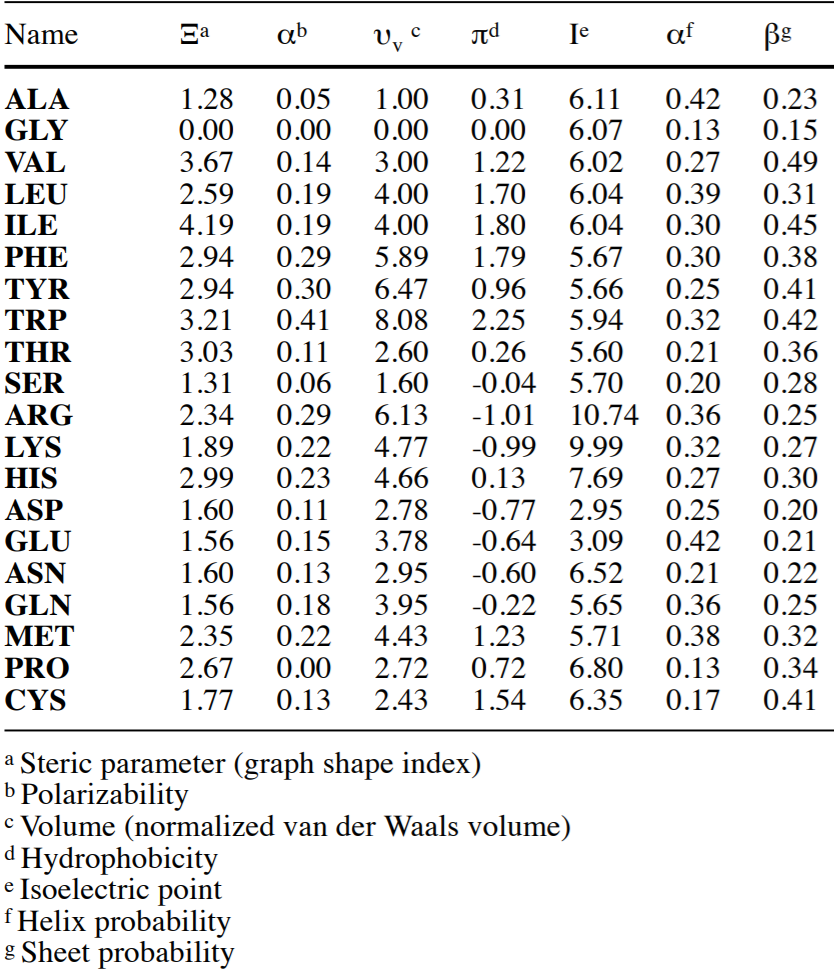
\includegraphics[width=0.7\textwidth]{tex/append/PPamino}
	\end{center}
	\caption[Physical properties of amino acids.]{Physical properties of amino acids \cite{Meiler.2001}.}
	\label{fig:appendSSstruct}
\end{figure} 
\chapter{Disk }
\label{app:AppDisk}


Content of the Disk:


\begin{lstlisting}[language=C,numbers=none,
caption=Contents of the Disc,
label=fubarTest]
|---Data
    |---input
    |   |---database
    |   |---MSA
    |---roc
    |   |---ROC_Forward
    |   |   |---jpg
    |   |   |---ROC
    |   |---ROC_FOR_PCA
    |   |   |---jpg
    |   |   |---ROC
    |   |---ROC_Viterbi
    |   |   |---jpg
    |   |   |---ROC
    |   |---ROC_VitForPCA
    |   |   |---jpg
    |   |   |---ROC
    |   |---ROC_VIT_PCA
    |   |   |---jpg
    |   |   |---ROC
    |   |---RocScores
    |---scores
        |---AA
        |---DSSP_m1_025_1
        |---DSSP_m1_025_3
        |---DSSP_m2_025_1_3
        |---DSSP_m2_025_1_5
        |---DSSP_m3_025_1
        |---DSSP_m3_025_3
        |---DSSP_m3_100_1
        |---DSSP_m3_100_5
        |---SSP_msa_c.67.1
\end{lstlisting}
\chapter{MSA c.67.1}
\label{app:MSAc671}

%\lstset{
%basicstyle  = \footnotesize,
% \singlespacing }%oder numbers=left
\begin{lstlisting}[basicstyle=\scriptsize\ttfamily, caption=MSA c.67.1,label=abbMSA67]
# STOCKHOLM 1.0

d1vefa1 ...WRALLEAEKTLDSG........VYNKHDLLIVRGQGARVWDAEGNEYIDCVGGYGVANLGHGNPEVVEAVKRQAET.
d2epja_ GEKSRMLFERTKELFPGGVNSPVRAAVKPYPFYVKRGEGAYLYTVDGARIVDLVLAYGPLILGHKHPRVLEAVEEALARG
d1zoda_ .......LNDDATFWRNARHHLVRYGGTFEPMIIERAKGSFVYDADGRAILDFTSGQMSAVLGHCHPEIVSVIGEYAGK.
d3doda_ ...HDLIEKSKKHLWLP...FTQMKDYDENPLIIESGTGIKVKDINGKEYYDGFSSVWLNVHGHRKKELDDAIKKQLGK.
d1fg7a_ ..............................TVTITDLARENVRNLTPYQSARRLGGNGDVWLNAN..EYPTAVEFQLTQQ
d2f8ja_ ..............................HMNPLDLIAKRAYPYETEKRDKTYLALNENPFPFP.EDLVDEVFRRLNSD
d1lc5a_ ..............................LFNTAHGGNIREPATVLGISPDQLLDFSANINPLG.MPVSVKRALIDNLD
d1bw0a_ ........WDVSMSNHAGLVFNPIRTVSDNAKPSPSPKPIIKLSVGDPTLDKNLLTSAAQIKKLKEAIDSQECNGYFPTV
d2gb3a1 ........................FSDRVLLTEESPIRKLVPFAEMAKKRGVRIHHLNIGQPDLKTPEVFFERIYENKPE
d2dkja_ ....................KRDEALFELIALEEKRQREGLELIASENFVSKQVREAVGSVLTNKYAEGYPGARYYGGCE
d2ez1a_ ...............NYPAEPFRIKSVETVSMIPRDERLKKMQEAGYNTFLLNSKDIYIDLLTDSGTNAMSDKQWAGMMM
d2rfva_ ...............................SDXRTYGFNTQIVHAGQQPDPSTGALSTPIFQTSTFVFDSAEQGAARFG
d2c81a_ ............................WPEWPQHSDRTRRKIEEVFQSNRWAISGYWTGEESMERKFAKAFADFNGVPY
d3k40a_ .............MEAPEFKDFAKTMVDFIAEYLENIRERRVLPEVKPGYLKPLIPDAAPEKPEKWQDVMQDIERVIMPG
d1m32a_ .............................YLLLTPGPLTTSRTVKEAMLFDSCTWDDDYNIGVVEQIRQQLTALATASEG

d1vefa1 .LMAMPQ..TLPTPMRGEFYRTLT..AILPPELNRVFPVNSGTEANEAALKFARAHTGRKKFVAAMRGFSGRTMGSLSVT
d2epja_ WLYGAPG..EAEVLLAEKILG.......YVKRGGMIRFVNSGTEATMTAIRLARGYTGRDLILKFDGCYHGSHDAVLVAA
d1zoda_ .LDHLFS..EMLSRPVVDLATRLA..NITPPGLDRALLLSTGAESNEAAIRMAKLVTGKYEIVGFAQSWHGMTGAAASAT
d3doda_ IAHSTLL..GMTNVPATQLAETLI..DISPKKLTRVFYSDSGAEAMEIALKMAFQYWKNIGKPEKQKFIAMKSYKAPIPY
d1fg7a_ TLNRYPE..CQPKAVIENYAQ.......YAGVKPEQVLVSRGADEGIELLIRAFCEPGKDAILYCPPTYGMYSVSAETIG
d2f8ja_ ALRIYYD..SPDEELIEKILSYLD..TDFLSKNN..VSVGNGADEIIYVMMLMFDRS.....VFFPPTYSCYRIFAKAVG
d1lc5a_ CIERYPD..ADYFHLHQALAR.......HHQVPASWILAGNGETESIFTVASGLKPR...RAMIVTPGFAEYGRALAQSG
d1bw0a_ GSPEARE..AVATWWRNSFVHKEE..LKSTIVKDNVVLCSGGSHGILMAITAICDAG..DYALVPQPGFPHYETVCKAYG
d2gb3a1 VVYYSHS..AGIWELREAFASYYKRRQRVDVKPENVLVTNGGSEAILFSFAVIANPG..DEILVLEPFYANYNAFAKIAG
d2dkja_ VIDRVES..LAIERAKALFGAAWAN...........VQPHSGSQANMAVYMALMEPG..DTLMGMDLAAGGHLTHGSRVN
d2ez1a_ GDEAYAG..SENFYHLERTVQELFG.....FKHIVPTHQGRGAENLLSQLAIKPGQYVAGNMYFTTTRYHQEKNGAVFVD
d2rfva_ YIYTRLG..NPTTDALEKKLAVLE.......RGEAGLATASGISAITTTLLTLCQQG..DHIVSASAIYGCTHAFLSHSM
d2c81a_ CVPTTSG..STALMLALEALGIGEG....DEVIVPSLTWIATATAVLNVNALPVFVDVEADTYCIDPQLIKSAITDKTKA
d3k40a_ VTHWHSPKFHAYFPTANSYPAIVADMLSGAIACIGFTWIASPACTELEVVMMDWLGKMLELPAEFLACSGGKGGGVIQGT
d1m32a_ YTSVLLQ..GSGSYAVEAVLGSALG......PQDKVLIVSNGAYGARMVEMAG........LMGIAHHAYDCGEVARPDV

d1vefa1 .WEPKYREPFLPLVEPVEFIPYNDVEALKR................AVDEE...TAAVILEPVQGEGGVRPATPEFLRAA
d2epja_ GGVPTSAGVPEAVARLTLVTPYNDVEALER................VFAEYGDRIAGVIVEPVIANAGVIPPRREFLAAL
d1zoda_ YSAGRKGVGPAAVGSFAIPAPFTYRPRFERNGAYDYLAELDYAFDLIDRQSSGNLAAFIAEPILSSGGIIELPDGYMAAL
d3doda_ VYRSESGDPDECRDQCLRELAQLLEEHHEE.......................IAALSIESMVQGASGMIVMPEGYLAGV
d1fg7a_ .....VECRTVPTLDNWQLDLQGISDKLDG.......................VKVVYVCSPNNPTGQLINPQD..FRTL
d2f8ja_ .....AKFLEVPLTKDLRIPEVNVGE...........................GDVVFIPNPNNPTGHVFEREE......
d1lc5a_ ...CEIRRWSLREADGWQLTDAILEALTPD.......................LDCLFLCTPNNPTG..LLPERPLLQAI
d1bw0a_ ...IGMHFYNCRPENDWEADLDEIRRLKDD......................KTKLLIVTNPSNPCGSNFSRKH..VEDI
d2gb3a1 ...VKLIPVTRRMEEGFAIPQNLESFINER.......................TKGIVLSNPCNPTGVVYGKDE..MRYL
d2dkja_ ....FSGKLYKVVSYGVRPDTELIDLEEVR.......................RLALEHRPKVIVAGASAYPRFWDFKAF
d2ez1a_ IVRDEAHDAGLNIAFKGDIDLKKLQKLIDE...................KGAENIAYICLAVTVNLAGGQPVSMANMRAV
d2rfva_ P....KFGINVRFVDAAKPEEIRAAMRPET........................KVVYIETPANPTLSLVDIET.....V
d2c81a_ IIPVHLFGSMANMDEINEIAQEHNLFVIED......................CAQSHGSVWNNQRAGTIGDIGAFSCQQG
d3k40a_ ASESTLVALLGAKAKKLKEVKELHPEWDEHTILG..................KLVGYCSDQAHSSVERAGLLGGVKLRSV
d1m32a_ QAIDAILNADPTISHIAMVHSETTTGMLNP.......................IDEVGALAHRYGKTYIVDAMSSFGGIP

d1vefa1 REITQEKGALLILDEIQTGMG......RTGKRFAFEHFGIVPDILTLAKA..LGGG.VPLGVAVMREEVARSMPKGG...
d2epja_ QRLSRESGALLILDEVVTGF.......RLGLEGAQGYFNIEGDIIVLGKI..IGGG.FPVGAVAGSREVMSLLTPQGK..
d1zoda_ KRKCEARGMLLILDEAQTGVG......RTGTMFACQRDGVTPDILTLSKT..LGAG.LPLAAIVTSAAIEERAHELG...
d3doda_ RELCTTYDVLMIVDEVATGFG......RTGKMFACEHENVQPDLMAAGKG..ITGGYLPIAVTFATEDIYKAFYDDYENL
d1fg7a_ LELTRGKAIVVADEAYIEFCP......QASLAGWLAEYPHLAILRTLSKA..FALAGLRCGFTLANEEVINLL.......
d2f8ja_ IERILKTGAFVALDEAYYEFH......GESYVDFLKKYENLAVIRTFSKA..FSLAAQRVGYVVASEKFIDAYN......
d1lc5a_ ADRCKSLNINLILDEAFIDFIPH....ETGFIPALKDNPHIWVLRSLTKF..YAIPGLRLGYLVNSDDAAMARMR.....
d1bw0a_ VRLAEELRLPLFSDEIYAGMVFKGKDPNATFTSVADFETTVPRVILGGTAXNLVVPGWRLGWLLYVDPHGNGPSFLEG..
d2gb3a1 VEIAERHGLFLIVDEVYSEIVFR.....GEFASALSIESDKVVVIDSVSX.KFSACGARVGCLITRNEELISHAMKLA..
d2dkja_ REIADEVGAYLVVDMAHFAGLVAAGLHPNPLPYAHVVTSTTHKTLRGPRGGLILSNDPELGKRIDKLIFPGIQGGP....
d2ez1a_ RELTEAHGIKVFYDATRCVENAYFIKEQEQGFENKSIAEIVHEMFSYADG...CTMSGKXDCLVNIGGFLCMNDDEMFSS
d2rfva_ AGIAHQQGALLVVDNTFMSPY.....CQQPLQLGADIVVHSVTXYINGHGDVIGGIIVGKQEFIDQARFVGLKDITGGCM
d2c81a_ KVLTAGEGGIIVTKNPRLFELIQQLRADSRVYCDDSSELMHGDMQLVKKG.DIQGSNYCLSEFQSAILLDQLQELDDK..
d3k40a_ QSENHRMRGAALEKAIEQDVAEGLIPFYAVVTLGTTNSCAFDYLDECGPVGNKHNLWIHVDAAYAGSAFICPEYRHLMKG
d1m32a_ MDIAALHIDYLISSANKCIQG......VPGFAFVIAREQKLAACKGHSRS.......LSLDLYAQWRCMEDNHG......

d1vefa1 .....HGTTFGGNPLAMAAGVAAIRYLERTRLWERAAELGPWFMEKLRAIPSPK......IREVRG.MGLMVGLELKEK.
d2epja_ ...VFNAGTFNAHPITMAAGLATLKALEEEPVYSVSREAAKALEEAASEVLDRTGLPYTINRVESM.MQLFIGVEEVSN.
d1zoda_ ...YLFYTTHVSDPLPAAVGLRVLDVVQRDGLVARANVMGDRLRRGLLDLMERFD....CIGDVRG.RGLLLGVEIVKDR
d3doda_ K.TFFHGHSYTGNQLGCAVALENLALFESENIVEQVAEKSKKLHFLLQDLHALPH.....VGDIRQ.LGFMCGAELVRSK
d1fg7a_ ......MKVIAPYPLSTPVADIAAQALSPQGIVAMRERVAQIIAEREYLIAALKEIPCVEQVFDSE.TNYILARFKASS.
d2f8ja_ .......RVRLPFNVSYVSQMFAKVALDHREIFEERTKF..IVEERERMKSALREMG..YRITDSR.GNFVFVFMEKEE.
d1lc5a_ .......RQQMPWSVNALAALAGEVALQDS..AWQQATWHWLREEGARFYQALCQLP.LLTVYPGR.ANYLLLRCERED.
d1bw0a_ ....LKRVGMLVCGPCTVVQAALGEALLNTPQEHLDQIVAKIEESAMYLYNHIGECIGLAPTMPRG.AMYLMSRIDLEKY
d2gb3a1 .......QGRLAPPLLEQIGSVGLLNLDDSFFDFVRETYRERVETVLKKLEEHGLKR...FTKPSG.AFYITAELPVEDA
d2dkja_ .....LEHVIAGKAVAFFEALQPEFKEYSRLVVENAKRLAEELARRGYRIVTGGTDNHLFLVDLRP.KGLTGKEAEERLD
d2ez1a_ A.KELVVVYEGMPSYGGLAGRDMEAMAIGLREAMQYEYIEHRVKQVRYLGDKLKAAGVPIVEPVGG.HAVFLDARRFCEH
d2rfva_ SPFNAWLTLRGVKTLGIRMERHCENALKIARFLEGHPSITRVYYPGLSSHPQYELGQRQMSLPGGI.ISFEIAGGLEAGR
d2c81a_ ...NAIREKNAMFLNDALSKIDGIKVMKRPPQVSRQTYYGYVFRFDPVKFGGLNADQFCEILREKLNMGTFYLHPPYLPV
d3k40a_ .IESADSFNFNPHXWMLVNFDCSAMWLKDPSWVPLGRRFRALKLWFVLRLYGVENLQAHIRRHCNFAKQFGDLCVADSRF
d1m32a_ .....KWRFTSPTHTVLAFAQALKELAKEGGVAARHQRYQQNQRSLVAGMRALGFNTLLDDELHSPIITAFYSPEDPQYR

d1vefa1 ....AAP........YIARLEKEHRVLALQAGPT............VIR.FLPPLVIEKEDLERVVEAVRAVLA......
d2epja_ ....AAQARKADKKFYVKLHEEMLRRGVFIAPSN............LEA.VFTGLPHQGEALEIAVEGLRSSLKTVLGS.
d1zoda_ RTKEPADGLGAKITRECMNLGLSMNIVQLPGMGG............VFR.IAPPLTVSEDEIDLGLSLLGQAIERAL...
d3doda_ ..ETKEPYPADRRIGYKVSLKMRELGMLTRPLGD............VIA.FLPPLASTAEELSEMVAIMKQAIHEVTSLE
d1fg7a_ .............AVFKSLWDQGIILRDQNKQPS............LSG.CLRITVGTREESQRVIDALRAEQV......
d2f8ja_ .................KERLLEHLRTKNVAVRS............FRE.GVRITIGKREENDMILRELEVF........
d1lc5a_ ............IDLQRRLLTQRILIRSCANYPG............LDSRYYRVAIRSAAQNERLLAALRNVL.......
d1bw0a_ R......DIKTDVEFFEKLLEEENVQVLPGTIFH............APGFTRLTTTRPVEVYREAVERIKAFCQRHAA..
d2gb3a1 EEFAR..WMLTDFNMDGETTMVAPLRGFYLTPGL............GKKEIRIACVLEKDLLSRAIDVLMEGLKMFCS..
d2dkja_ AVGITVNKNAIPFDPKPPRVTSGIRIGTPAITTRGFT.........PEEMPLVAELIDRALLEGPSEALREEVRRLALAH
d2ez1a_ LTQDEFPAQSLAASIYVETGVRSMERGIISAGRNNVTGEHHRPKLETVRLTIPRRVYTYAHMDVVADGIIKLYQHKEDIR
d2rfva_ RMINSVELCLLAVSLGDTETLIQHPASMTHSPVAPEER.....LKAGITDGLIRLSVGLEDPEDIINDLEHAIRKAT...
d2c81a_ HKNPLFCPWTKNRYLKSVRKTEAYWRGLHYPVSERASG.......QSIVIHHAILLAEPSHLSLLVDAVAELARKFCV..
d3k40a_ ELAAEINMGLVCFRLKGSNERNEALLKRINGRGHIHLVPAKIKDVYFLRMAICSRFTQSEDMEYSWKEVSAAADEMEQEQ
d1m32a_ ...........FSEFYRRLKEQGFVIYPGKVSQS............DCFRIGNIGEVYAADITALLTAIRTAMYWT....

d1vefa1 .....................
d2epja_ .....................
d1zoda_ .....................
d3doda_ D....................
d1fg7a_ .....................
d2f8ja_ .....................
d1lc5a_ .....................
d1bw0a_ .....................
d2gb3a1 .....................
d2dkja_ PMP..................
d2ez1a_ GLKFIYEPKQLRFFTARFDYI
d2rfva_ .....................
d2c81a_ .....................
d3k40a_ .....................
d1m32a_ .....................
//


\end{lstlisting}
\chapter{Comparision of Scatterplots for MSA c.67.1 }
\label{app:APPPCAcorrScores}

\begin{figure}[ht]
	\begin{center}
		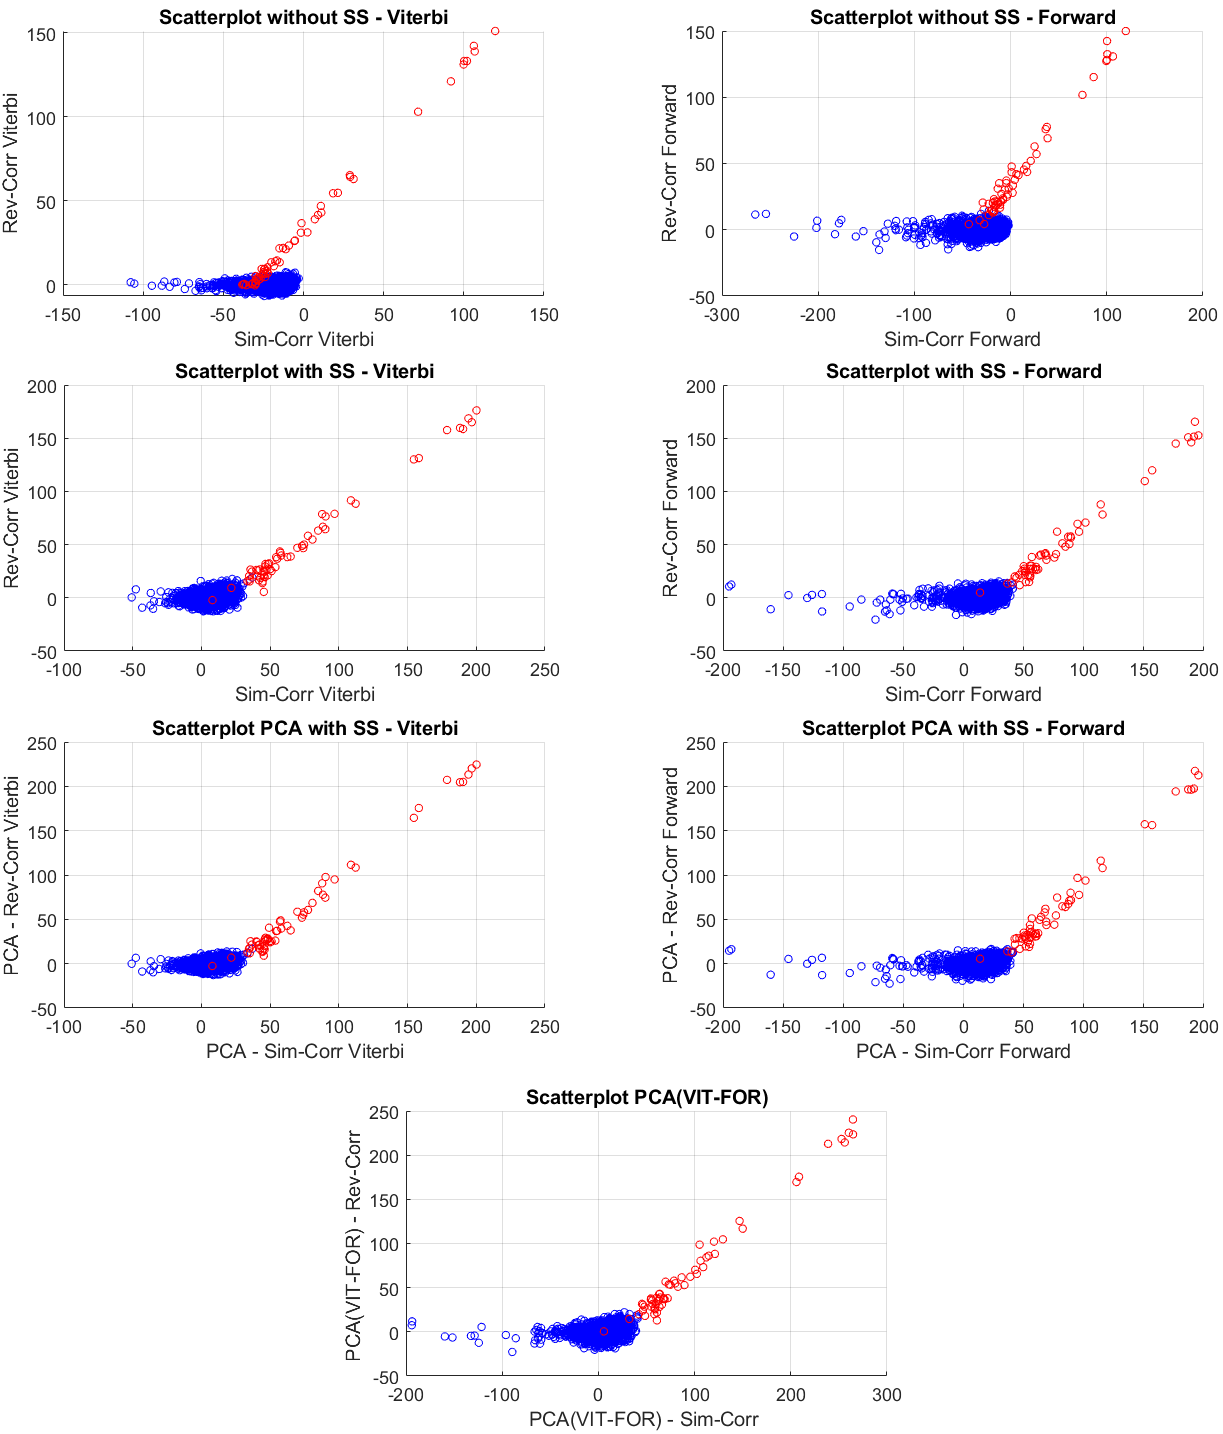
\includegraphics[width=0.94\textwidth]{tex/append/APP_SCATTER_c_67_1_v1}
	\end{center}
	\caption{Comparision of scatterplots for optimized scores of \acs{MSA} c.67.1.}
	\label{fig:APPSCATTERCOMPXX}
\end{figure} 
\chapter{Scatterplots for MSA c.67.1 used for ROC }
\label{app:APPPCAcorrScoresWeight}

\rotatebox{90}{\begin{minipage}{0.93\textheight}
    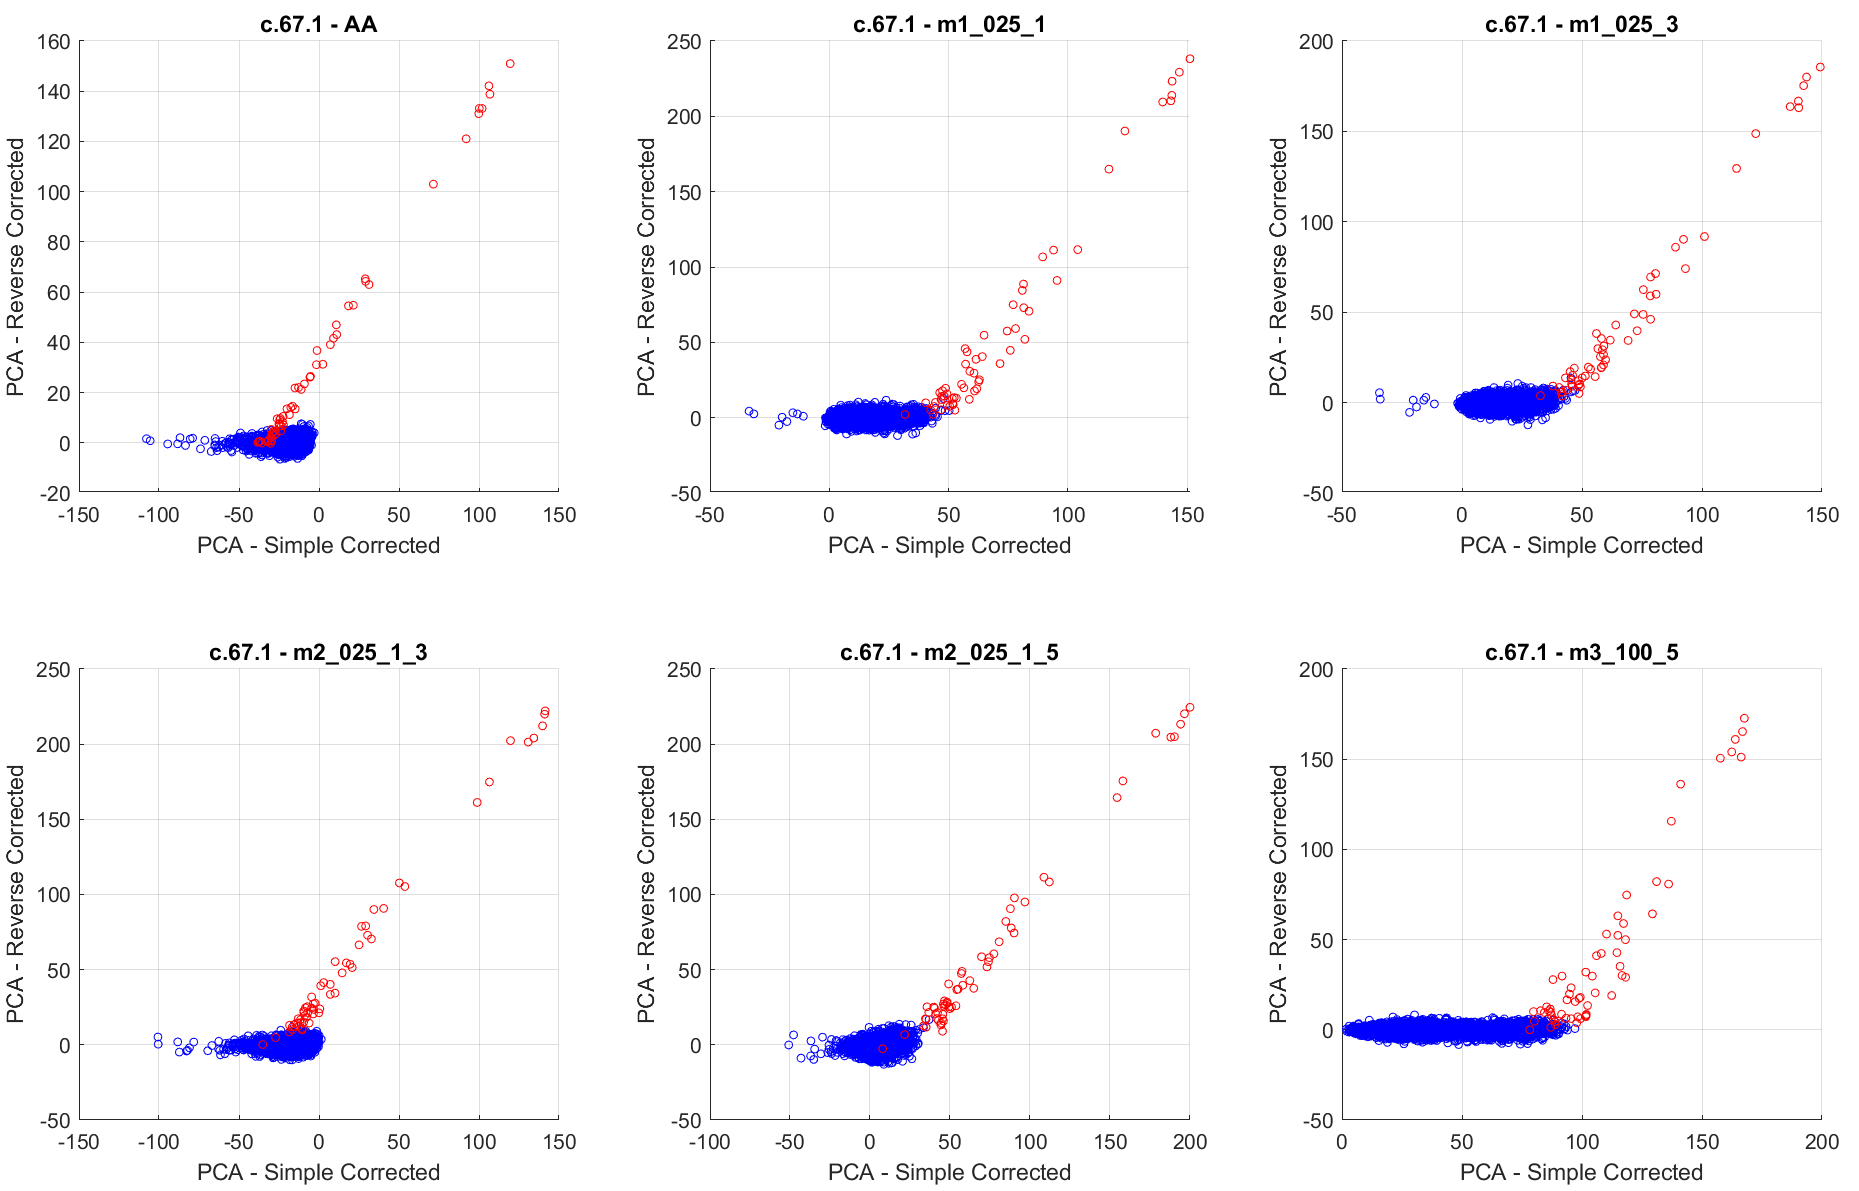
\includegraphics[width=\textwidth]{tex/append/c_67_1_PCAVIT}
    \captionof{figure}{Scatterplots of \acs{MSA} c.67.1 using different weighting methods.}

    \label{fig:APPSCATTERCOMPX}
\end{minipage}}
%\end{landscape} 

%\include{tex/append/PCA_Scores}
\end{appendix}


%\listoftodos[TODO Notes]

\end{document}
